%%%%%%%%%%%%%%%
%
% $Autor: Wings $
% $Datum: 2020-02-24 14:30:26Z $
% $Pfad: PythonPackages/PythonPackages/PythonPackages.tex $
% $Version: 1792 $
%
% !TeX encoding = utf8
% !TeX root = PythonPackages
% !TeX TXS-program:bibliography = txs:///bibtex
% !TeX program = LuaLaTeX
%
%
%%%%%%%%%%%%%%%




%%%%%%%%%%%%%%%
%
% Auswahl der Sprache
% Die nicht gewünschte Sprache muss auskommentiert werden:
%\def\isGerman{1}
\def\isEnglish{1}
%
%%%%%%%%%%%%%%%


\documentclass[10pt,a4paper,bibliography=totoc]{scrbook}

\usepackage[backend=biber, style=alphabetic]{biblatex} % Correct way to specify a style


\input{../General/packages}
\input{../General/commands}
\input{../General/Hyphenations}
\input{../General/tikzdefs}

\input{../General/acronyms}
\input{../General/Hyphenations}%

%\bibliography{Jetson} 
%\addbibresource{MyLiterature}
\addbibresource{MyLitManoj.bib}



\begin{document}


  \input{../Contents/PythonPackages/Titlepage}

  \tableofcontents
  \newpage

  \listoffigures
  \newpage

  \InputLanguage{../Contents/General/}{Acronymlist}
  \newpage



  
\part{Python Packages}

%  \InputLanguage{../Contents/General/}{PackageExample}
  
%  \InputLanguage{../Contents/General/}{Matplotlib}

%  \InputLanguage{../Contents/General/}{Flask}

%  \InputLanguage{../Contents/General/}{OpenCV}
  
  %\InputLanguage{../Contents/General/}{Pendulum}

%  \InputLanguage{../Contents/General/}{logging}
  
%  %%%%%%%%%%%%
%
% $Autor: Wings $
% $Datum: 2019-03-05 08:03:15Z $
% $Pfad: PythonPackages/Contents/General/PixelLib $
% $Version: 4250 $
% !TeX spellcheck = en_GB/de_DE
% !TeX encoding = utf8
% !TeX root = filename 
% !TeX TXS-program:bibliography = txs:///biber
%
%%%%%%%%%%%%



\chapter{Package \PYTHON{PixelLib}}

\section{Introduction}

PixelLib is a Python package specifically crafted to facilitate image and video segmentation within the domain of computer vision. Image segmentation, a pivotal task in computer vision, involves the partitioning of an image into discernible segments or regions based on specific characteristics such as color, texture, or spatial relationships. This segmentation process is crucial for tasks like object recognition, scene understanding, and overall visual content analysis.

By leveraging PixelLib, developers and researchers can streamline and expedite the segmentation process, making it more accessible for various applications. The library's capabilities extend to both images and videos, allowing for comprehensive segmentation analysis in dynamic visual scenarios. With PixelLib, intricate computer vision tasks become more manageable, providing a valuable tool for extracting meaningful insights from visual data.

\section{Detailed Description}
PixelLib supports two major types of segmentation:

\begin{itemize}
    \item \textbf{Semantic Segmentation:} This involves labeling each pixel in an image with a class of what is being represented. Pixels that are part of the same object type get the same label. PixelLib makes semantic segmentation accessible, with support for various pre-trained models.
    
    \item \textbf{Instance Segmentation:} Unlike semantic segmentation, instance segmentation not only labels each pixel of the image but also differentiates between different instances of the same class. This is particularly useful in scenarios where the distinction between individual objects of the same type is crucial.\newline
    
    Furthermore, PixelLib can also be used for background editing in images and videos.
    
    PixelLib supports two deep learning libraries for image segmentation which are Pytorch and Tensorflow.
\end{itemize}

\section{PixelLib Pytorch Version}

The pytorch version of PixelLib uses PointRend object segmentation architecture to replace Mask R-CNN for performing instance segmentation of objects. PointRend is an excellent state of the art neural network for implementing object segmentation. It generates accurate segmentation masks and run at high inference speed that matches the increasing demand for an accurate and real time computer vision applications. PixelLib is a library built to provide support for different operating systems.The PointRend implementation used for PixelLib supports both Linux and Windows OS.

\begin{figure}[h!]
    \centering
    \includegraphics[width=0.8\linewidth]{Images/PixelLib/pytorch1.png} % Adjust the path accordingly
    
    \caption{Mask R-CNN vs PointRend}
    \label{fig:your_image_label}
    
    
\end{figure}

\begin{figure}[h!]
    \centering
    \includegraphics[width=0.8\linewidth]{Images/PixelLib/pytorch2.png} % Adjust the path accordingly
    
    \caption{Mask R-CNN vs PointRend}
    \label{fig:your_image_label}
    
    
\end{figure}


The sample images above are examples of the differences in the segmentation results of PointRend compared to Mask RCNN. It is obvious that the PointRend image results are better segmentation outputs compared to Mask R-CNN results.

\section{Install PixelLib and its dependencies}

Download Python
PixelLib pytorch version supports python version 3.7 and above. Download a \url{https://www.python.org}.\newline


\textbf{Install Pytorch}\newline
PixelLib Pytorch version supports these versions of pytorch(1.6.0, 1.7.1,1.8.0 and 1.9.0).
Note: Pytorch 1.7.0 is not supported and do not use any pytorch version less than 1.6.0. Install a compatible\url{https://pytorch.org}

\textbf{Install Pycocotools}
\begin{verbatim}
    pip3 install pycocotools
\end{verbatim}

\textbf{Install PixelLib}
\begin{verbatim}
    pip3 install pixellib
\end{verbatim}	

If installed, upgrade to the latest version using:
\begin{verbatim}
    pip3 install pixellib — upgrade
\end{verbatim}		

\section{Examples of Semantic Image Segmentation}
PixelLib makes it possible to perform state of the art semantic segmentation of 150 classes of objects with Ade20k model using 5 Lines of Code. Perform indoor and outdoor segmentation of scenes with PixelLib by using Ade20k model.
\begin{figure}[h!]
    \centering
    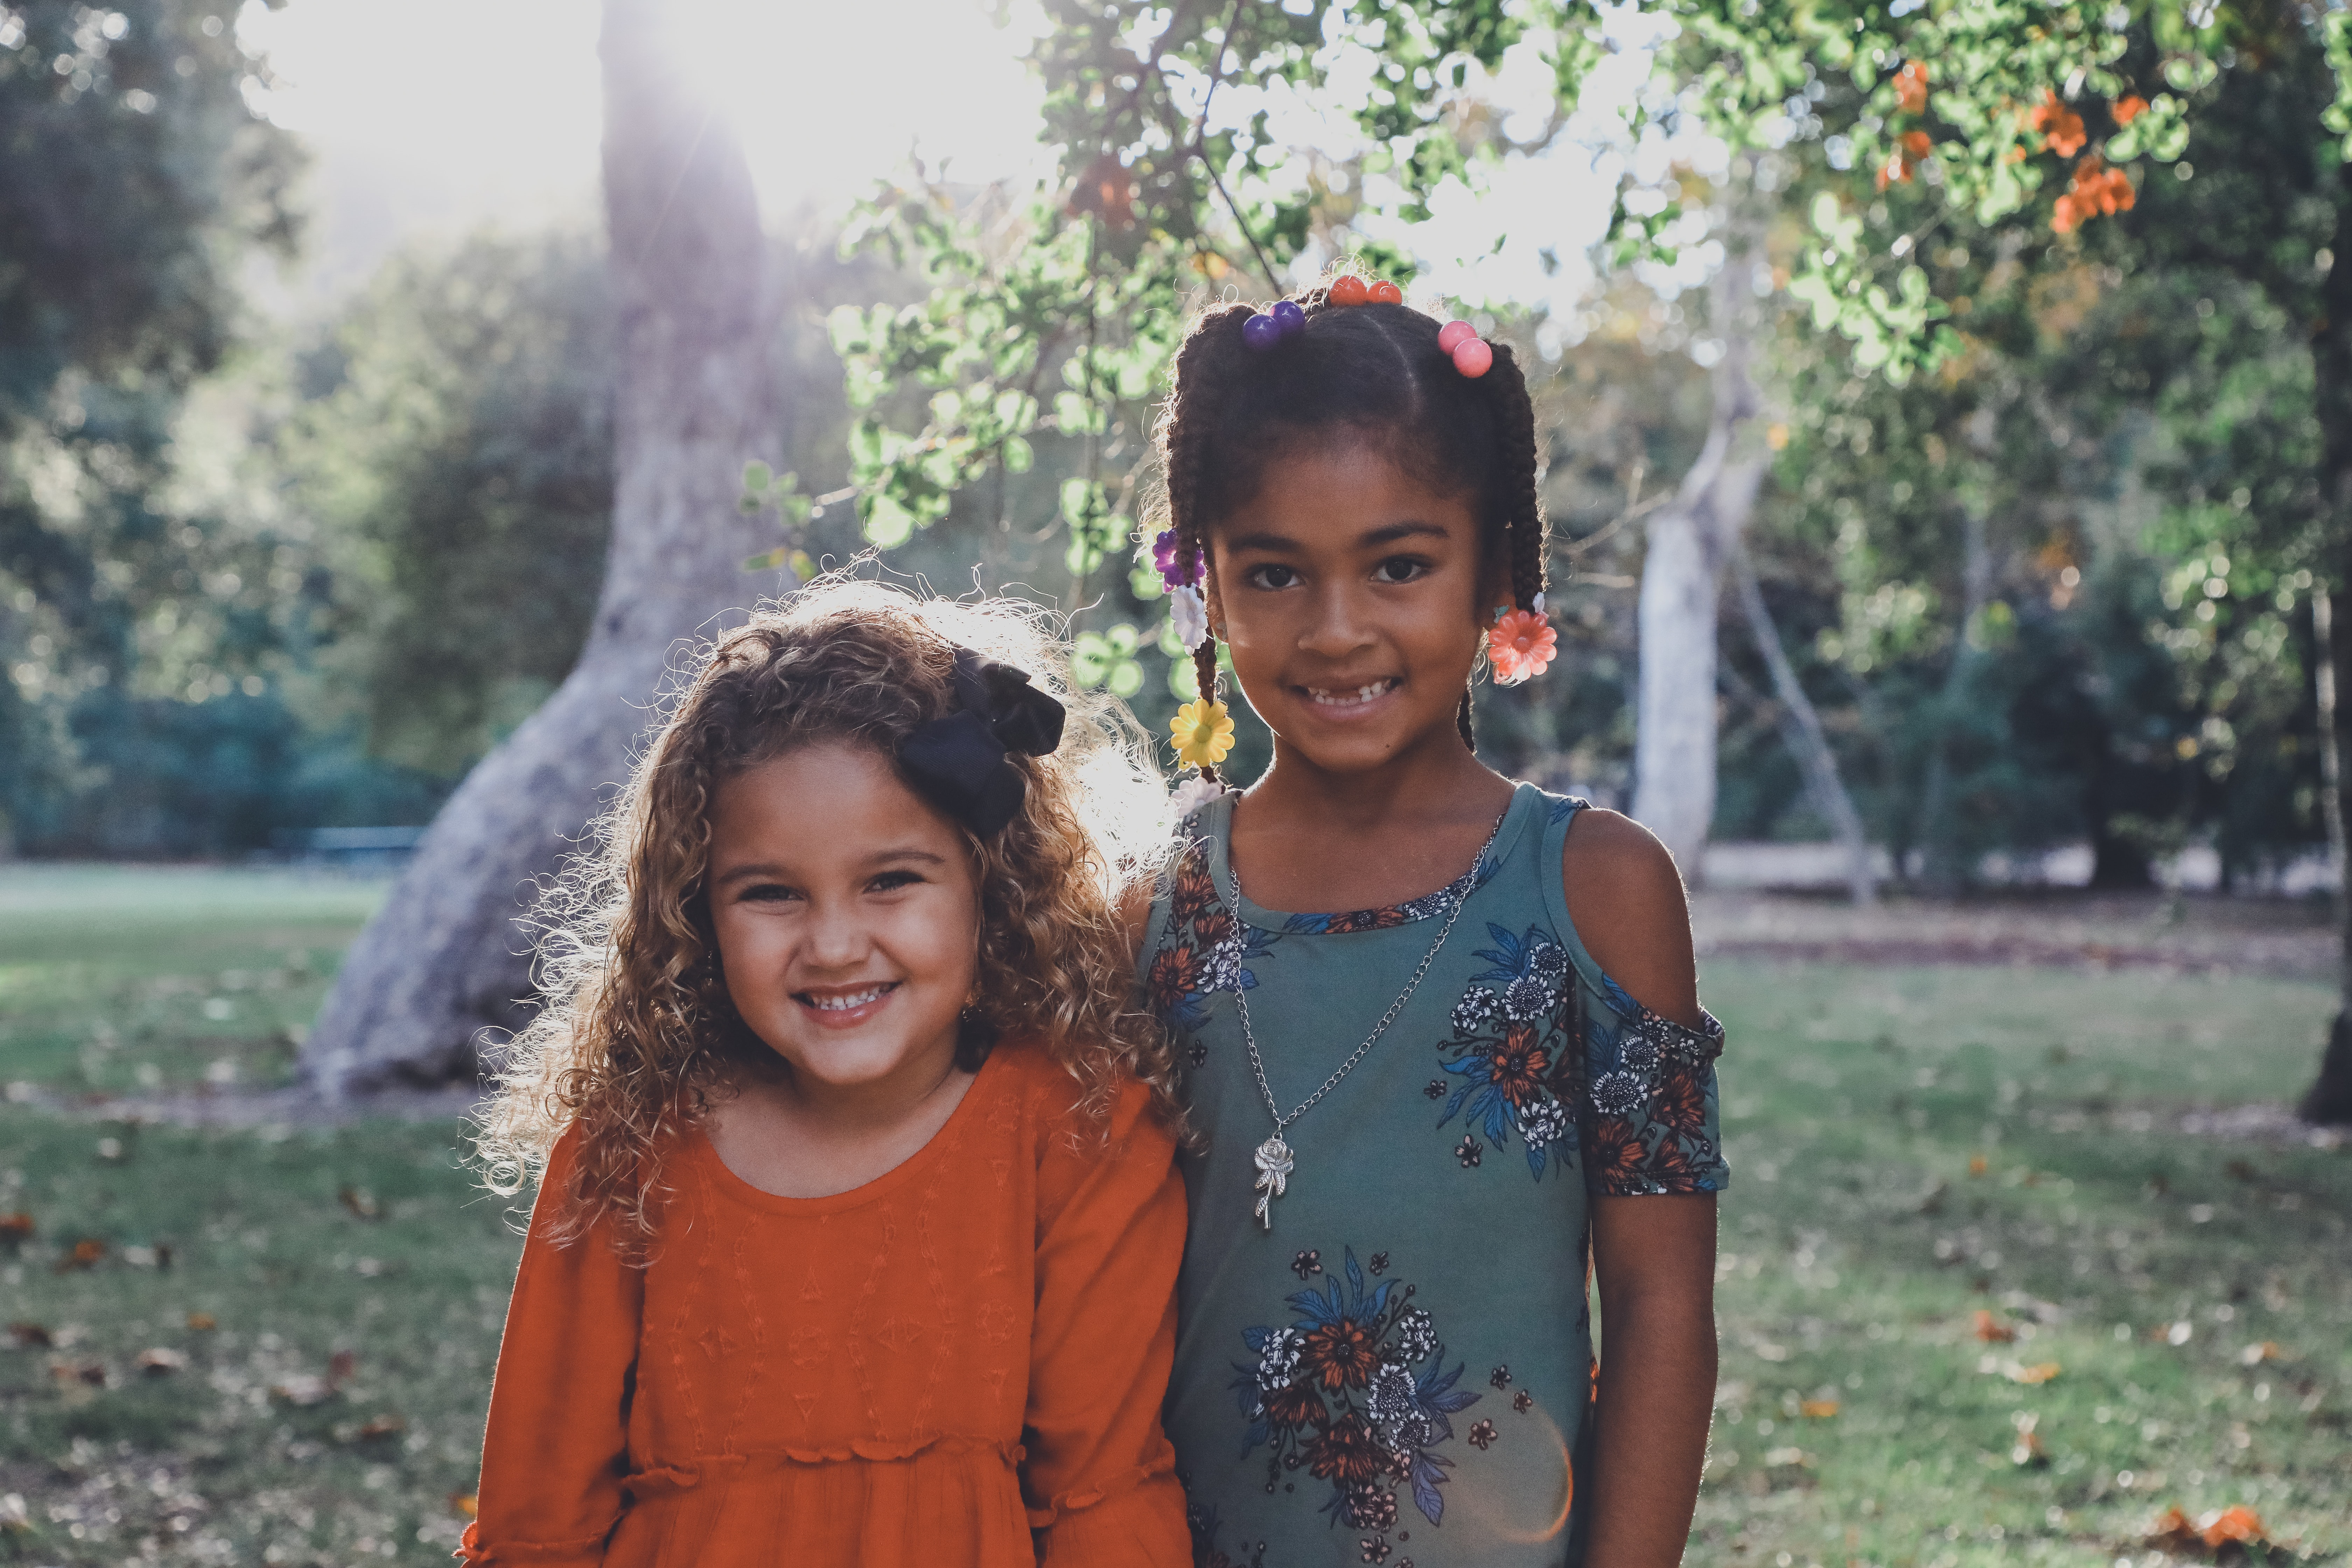
\includegraphics[width=0.8\linewidth]{Images/PixelLib/sem3.jpg} % Adjust the path accordingly
    
    \caption{Semantic Image Segmentation}
    \label{fig:your_image_label}
    
    
\end{figure}



\subsection{Example Manual}

Semantic Segmentation with Pixellib

\subsection{Description}
This example demonstrates how to use the Pixellib library for semantic segmentation of images using a pre-trained ADE20K model.

\subsection{Files}

\begin{itemize}
    \item \texttt{segmentation\_example.py}: Python script containing the code snippet.
    \item \texttt{deeplabv3\_xception65\_ade20k.h5}: Pre-trained ADE20K model.
    \item \texttt{sample.jpg}: Input image for semantic segmentation.
    \item \texttt{image\_new.jpg}: Output image with segmentation overlay.
\end{itemize}

\subsection{Version}

PixelLib semantic image segmentation supports Python 3.6 and above.

\subsection*{Supported Python Versions}

\begin{itemize}[label=--]
    \item \textbf{TensorFlow version:} PixelLib's TensorFlow version works with Python 3.6 and above.
    \item \textbf{PyTorch version:} This version also supports Python 3.7 and above.
\end{itemize}

\textbf{No additional PyTorch version constraints:} Unlike video segmentation, PyTorch version compatibility is not an issue for image segmentation. As long as you have Python 3.7 or above, you can use any supported PyTorch version.

\subsection*{Choosing the Right Version}

\begin{itemize}[label=--]
    \item \textbf{TensorFlow vs. PyTorch:} Both versions offer semantic image segmentation. Choose TensorFlow if you prioritize ease of use and have existing TensorFlow experience. Otherwise, PyTorch may offer more flexibility and customization.
\end{itemize}

\subsection*{Additional Resources}

\begin{itemize}[label=--]
    \item PixelLib GitHub repository: \url{https://github.com/ayoolaolafenwa/PixelLib}
    \item PixelLib official documentation: \url{https://pixellib.readthedocs.io/en/stable/}
    \item Real-Time Image Segmentation Using 5 Lines of Code: \url{https://towardsdatascience.com/tagged/image-segmentation}
\end{itemize}

\subsection{Example Code}

\begin{lstlisting}[language=Python]
    import pixellib
    from pixellib.semantic import semantic_segmentation
    
    # Create an instance of the semantic_segmentation class
    segment_image = semantic_segmentation()
    
    # Load a pre-trained ADE20K model (DeepLabV3 with Xception65 backbone)
    segment_image.load_ade20k_model("deeplabv3_xception65_ade20k.h5")
    
    # Perform semantic segmentation on the input image "sample.jpg"
    # Overlay the segmentation results on the original image and save as "image_new.jpg"
    segment_image.segmentAsAde20k("sample.jpg", overlay=True, output_image_name="image_new.jpg")
\end{lstlisting}


\subsection*{Code Description of Semantic Image Segmentation}

\textbf{Library and Module Import:}
\begin{itemize}
    \item \texttt{import pixellib:} Imports the \texttt{pixellib} library, which is a Python library for image and video segmentation tasks.
    \item \texttt{from pixellib.semantic import semantic\_segmentation:} Imports the \texttt{semantic\_segmentation} class from the \texttt{pixellib.semantic} module. This class is designed for performing semantic segmentation.
\end{itemize}

\textbf{Instance Creation:}
\begin{itemize}
    \item \texttt{segment\_image = semantic\_segmentation():} Creates an instance named \texttt{segment\_image} of the \texttt{semantic\_segmentation} class. This instance will be used to perform semantic segmentation on images.
\end{itemize}

\textbf{Model Loading:}
\begin{itemize}
    \item \texttt{segment\_image.load\_ade20k\_model("deeplabv3\_xception65\_ade20k.h5"):} Loads a pre-trained semantic segmentation model trained on the ADE20K dataset. The model is based on the DeepLabV3 architecture with the Xception65 backbone.
\end{itemize}

\textbf{Image Segmentation:}
\begin{itemize}
    \item \texttt{segment\_image.segmentAsAde20k("sample.jpg", overlay=True, output\_image\_name="image\_new.jpg"):} Performs semantic segmentation on the input image \texttt{"sample.jpg"} using the loaded ADE20K model. The segmentation results are overlaid on the original image if \texttt{overlay=True}. The processed image is then saved as \texttt{"image\_new.jpg"}.
\end{itemize}

\begin{figure}[h!]
    \centering
    \includegraphics[width=0.8\linewidth]{Images/PixelLib/a5.jpg} % Adjust the path accordingly
    
    \caption{Result of Semantic Image Segmentation}
    \label{fig:your_image_label}
    
    
\end{figure}

\section{Example of Semantic Video Segmentation}

\subsection{Example Manual}
Semantic Segmentation of Videos with Pixellib

\subsection{Description}
This example manual provides instructions on performing semantic segmentation on videos using the Pixellib library with a pre-trained ADE20K model. Semantic segmentation in videos involves labeling each pixel in every frame of the video with a corresponding class label, such as "road," "building," "sky," etc. The example demonstrates how to load the pre-trained model, process a video, and generate an output video with segmentation overlay on each frame.

\subsection{Example Files}
\begin{itemize}
    \item \texttt{semantic\_segmentation\_example.py}: Python script containing the code snippet.
    \item \texttt{deeplabv3\_xception65\_ade20k.h5}: Pre-trained ADE20K model.
    \item \texttt{sample\_video.mp4}: Sample input video for semantic segmentation.
    \item \texttt{output\_video.mp4}: Output video with segmentation overlay.
\end{itemize}

\subsection{Version}
PixelLib semantic video segmentation supports Python 3.7 and above.

\subsection*{PixelLib Versions}
\begin{itemize}[label=--]
    \item \textbf{TensorFlow version:} This version does not support video segmentation.
    \item \textbf{PyTorch version:} This version supports Python 3.7 and above, but requires compatible PyTorch versions:
    \begin{itemize}[label=$\bullet$]
        \item Supported versions: 1.6.0, 1.7.1, 1.8.0, and 1.9.0
        \item Unsupported version: 1.7.0 (avoid using)
        \item Versions less than 1.6.0: Not supported
    \end{itemize}
\end{itemize}

\subsection*{Choosing the Right Version}
\begin{itemize}[label=--]
    \item If you prioritize ease of use and minimal configuration, consider the TensorFlow version (not available for videos).
    \item If you need video segmentation and have more control over your environment, choose the PyTorch version and ensure compatibility with your PyTorch installation.
\end{itemize}

\subsection*{Additional Resources}
\begin{itemize}[label=--]
    \item PixelLib GitHub repository: \url{https://github.com/ayoolaolafenwa/PixelLib}
    \item PixelLib official documentation: \url{https://pixellib.readthedocs.io/en/stable/}
    \item Video segmentation with PixelLib (5 lines of code): \url{https://towardsdatascience.com/tagged/image-segmentation}
\end{itemize}

\subsection{Example Code}
\begin{lstlisting}[language=Python]
    import pixellib
    from pixellib.semantic import semantic_segmentation
    
    # Create an instance of the semantic_segmentation class for video processing
    segment_video = semantic_segmentation()
    
    # Load a pre-trained ADE20K model (DeepLabV3 with Xception65 backbone)
    segment_video.load_ade20k_model("deeplabv3_xception65_ade20k.h5")
    
    # Process a video named "sample_video.mp4" using ADE20K semantic segmentation
    # Overlay the segmentation results on each frame, display at 15 frames per second, and save as "output_video.mp4"
    segment_video.process_video_ade20k("sample_video.mp4", overlay=True, frames_per_second=15, output_video_name="output_video.mp4")
    
    
\end{lstlisting}


\subsection*{Code Description of Semantic Image Segmentation}




\textbf{Library Import:}
\begin{itemize}
    \item \texttt{import pixellib:} Imports the \texttt{pixellib} library, a Python library for image and video segmentation tasks.
    \item \texttt{from pixellib.semantic import semantic\_segmentation:} Imports the \texttt{semantic\_segmentation} class from the \texttt{pixellib.semantic} module. This class is designed for semantic segmentation tasks.
\end{itemize}

\textbf{Instance Creation:}
\begin{itemize}
    \item \texttt{segment\_video = semantic\_segmentation():} Creates an instance named \texttt{segment\_video} of the \texttt{semantic\_segmentation} class. This instance will be used for processing semantic segmentation on a video.
\end{itemize}

\textbf{Model Loading:}
\begin{itemize}
    \item \texttt{segment\_video.load\_ade20k\_model("deeplabv3\_xception65\_ade20k.h5"):} Loads a pre-trained semantic segmentation model named "deeplabv3\_xception65\_ade20k.h5." This model is trained on the ADE20K dataset and is based on the DeepLabV3 architecture with the Xception65 backbone.
\end{itemize}

\textbf{Video Processing:}
\begin{itemize}
    \item \texttt{segment\_video.process\_video\_ade20k("sample\_video.mp4", overlay=True, frames\_per\_second=15, output\_video\_name="output\_video.mp4"):} Processes a video named "sample\_video.mp4" using the loaded ADE20K model. It performs semantic segmentation on each frame, overlays the segmentation results on the original frames (\texttt{overlay=True}), displays the processed video at 15 frames per second, and saves the output video as "output\_video.mp4."
\end{itemize}
\begin{figure}[h!]
    \centering
    \includegraphics[width=0.8\linewidth]{Images/PixelLib/sem4.jpeg} % Adjust the path accordingly
    
    \caption{Result of Semantic Video Segmentation}
    \label{fig:your_image_label}
\end{figure}


\newpage

\section{Examples of Instance Image Segmentation}


\begin{figure}[h!]
    \centering
    \includegraphics[width=0.8\linewidth]{Images/PixelLib/seg.jpeg} % Adjust the path accordingly
    
    \caption{Image segmentation using PointRed}
    \label{fig:your_image_label}
    
    
\end{figure}
\subsection{Example Manual}
Instance Segmentation with Pixellib

\subsection{Description}
This example manual provides instructions on performing instance segmentation on images using the Pixellib library with a pre-trained model. Instance segmentation is a computer vision task where objects in an image are not only classified into different classes but also segmented and individually identified. The example demonstrates how to load the pre-trained model, process an input image, and generate an output image with bounding boxes around segmented objects.

\subsection{Example Files}
\begin{itemize}
    \item \texttt{instance\_segmentation\_example.py}: Python script containing the code snippet.
    \item \texttt{pointrend\_resnet50.pkl}: Pre-trained model for instance segmentation.
    \item \texttt{image.jpg}: Sample input image for instance segmentation.
    \item \texttt{output\_image.jpg}: Output image with bounding boxes around segmented objects.
\end{itemize}

\subsection{Version}
Supported Python Versions and Dependencies for PixelLib Instance Image Segmentation

\subsection*{TensorFlow Version}
\begin{itemize}[label=--]
    \item \textbf{Python:} This version supports Python 3.5 and above, but it uses TensorFlow 2.x, so make sure you have a compatible version installed.
\end{itemize}

\subsection*{PyTorch Version}
\begin{itemize}[label=--]
    \item \textbf{Python:} This version supports Python 3.7 and above similar to semantic video segmentation.
    \item \textbf{PyTorch:} Similar to video segmentation, it requires specific PyTorch versions:
    \begin{itemize}[label=$\bullet$]
        \item Supported versions: 1.6.0, 1.7.1, 1.8.0, and 1.9.0
        \item Unsupported version: 1.7.0
        \item Versions less than 1.6.0: Not supported
    \end{itemize}
\end{itemize}

\subsection*{Choosing the Right Version}
\begin{itemize}[label=--]
    \item For simplicity and compatibility with older Python versions, choose the TensorFlow version if you don't need video segmentation.
    \item For faster performance and broader model selection, choose the PyTorch version, but ensure your Python and PyTorch versions are compatible.
\end{itemize}

\subsection*{Additional Resources}
\begin{itemize}[label=--]
    \item PixelLib GitHub repository: \url{https://github.com/ayoolaolafenwa/PixelLib}
    \item PixelLib official documentation: \url{https://pixellib.readthedocs.io/en/stable/}
\end{itemize}

\subsection{Example Code}
\begin{lstlisting}[language=Python]
    import pixellib
    from pixellib.torchbackend.instance import instanceSegmentation
    
    # Create an instance of the instanceSegmentation class
    ins = instanceSegmentation()
    
    # Load a pre-trained model named "pointrend_resnet50.pkl"
    ins.load_model("pointrend_resnet50.pkl")
    
    # Perform instance segmentation on the input image "image.jpg"
    # Show bounding boxes on the segmented objects and save the output as "output_image.jpg"
    ins.segmentImage("image.jpg", show_bboxes=True, output_image_name="output_image.jpg")
\end{lstlisting}




\section*{Code description of Instance Image Segmentation}				
\begin{description}
    \item[Library Import:]
    \begin{itemize}
        \item \texttt{import pixellib:} Imports the \texttt{pixellib} library, a Python library for image and video segmentation tasks.
    \end{itemize}
    
    \item[Module Import:]
    \begin{itemize}
        \item \texttt{from pixellib.torchbackend.instance import instanceSegmentation:} Imports the \texttt{instanceSegmentation} class from the \texttt{pixellib.torchbackend.instance} module. This class is designed for performing instance segmentation using PyTorch.
    \end{itemize}
    
    \item[Instance Creation:]
    \begin{itemize}
        \item \texttt{ins = instanceSegmentation():} Creates an instance named \texttt{ins} of the \texttt{instanceSegmentation} class, initializing an object for performing instance segmentation.
    \end{itemize}
    
    \item[Model Loading:]
    \begin{itemize}
        \item \texttt{ins.load\_model("pointrend\_resnet50.pkl"):} Loads a pre-trained instance segmentation model named "pointrend\_resnet50.pkl." This model is based on the ResNet50 architecture and is designed for identifying and segmenting different instances (objects) within an image.
    \end{itemize}
    
    \item[Instance Segmentation:]
    \begin{itemize}
        \item \texttt{ins.segmentImage("image.jpg", show\_bboxes=True, output\_image\_name="output\_image.jpg"):} Performs instance segmentation on the input image "image.jpg" using the loaded model. It shows bounding boxes around the segmented objects (\texttt{show\_bboxes=True}) and saves the output image as "output\_image.jpg."
    \end{itemize}
\end{description}

\begin{figure}[h!]
    \centering
    \includegraphics[width=0.8\linewidth]{Images/PixelLib/seg2.jpeg} % Adjust the path accordingly
    
    \caption{Result of Image segmentation using PointRed}
    \label{fig:your_image_label}
    
    
\end{figure}
\newpage		



\section{Example of Instance Video Segmentation}
\subsection{Example Manual}
Instance Video Segmentation with Pixellib
\subsection{Description}
This example manual provides instructions on performing instance segmentation on images and videos using the Pixellib library with a pre-trained model. Instance segmentation is a computer vision task where objects in an image or video are not only classified into different classes but also segmented and individually identified. The example demonstrates how to load the pre-trained model, process input images and videos, and generate output with bounding boxes around segmented objects.

\subsection{Example Files}
\begin{itemize}
    \item \texttt{instance\_segmentation\_image.py}: Python script for image instance segmentation.
    \item \texttt{instance\_segmentation\_video.py}: Python script for video instance segmentation.
    \item \texttt{pointrend\_resnet50.pkl}: Pre-trained model for instance segmentation.
    \item \texttt{sample\_video.mp4}: Sample input video for instance segmentation.
    \item \texttt{image.jpg}: Sample input image for instance segmentation.
    \item \texttt{output\_image.jpg}: Output image with bounding boxes around segmented objects.
    \item \texttt{output\_video.mp4}: Output video with bounding boxes around segmented objects.
\end{itemize}

\subsection{Version}
Compatible Python and PyTorch Versions for PixelLib Instance Video Segmentation

\subsection*{Python Version}
\begin{itemize}[label=--]
    \item Supported: 3.7 and above
\end{itemize}

\subsection*{PyTorch Version}
\begin{itemize}[label=--]
    \item Supported: 1.6.0, 1.8.0, and 1.9.0
    \item Unsupported: 1.7.0 (avoid using)
    \item Versions less than 1.6.0: Not supported
\end{itemize}

\subsection*{Key Points}
\begin{itemize}[label=--]
    \item PixelLib's TensorFlow version does not currently support video segmentation.
    \item Only the PyTorch version offers video segmentation capabilities, including instance segmentation.
    \item Make sure your PyTorch installation aligns with the supported versions mentioned above.
\end{itemize}

\subsection*{Useful Resources}
\begin{itemize}[label=--]
    \item PixelLib GitHub repository: \url{https://github.com/ayoolaolafenwa/PixelLib}
    \item PixelLib official documentation: \url{https://pixellib.readthedocs.io/en/latest/}
    \item Video Segmentation With 5 Lines of Code: \url{https://towardsdatascience.com/video-segmentation-with-5-lines-of-code-87f798afb93}
\end{itemize}

\subsection{Example Code}	
\begin{lstlisting}[language=Python]
    import pixellib
    from pixellib.torchbackend.instance import instanceSegmentation
    
    # Create an instance of the instanceSegmentation class
    ins = instanceSegmentation()
    
    # Load a pre-trained model named "pointrend_resnet50.pkl"
    ins.load_model("pointrend_resnet50.pkl")
    
    # Process a video named "sample_video.mp4"
    # Show bounding boxes on the segmented objects, display 3 frames per second, and save the output as "output_video.mp4"
    ins.process_video("sample_video.mp4", show_bboxes=True, frames_per_second=3, output_video_name="output_video.mp4")
    
\end{lstlisting}


\subsection*{Code description of video segmentation}	
\begin{description}
    \item[Library Import:]
    \begin{itemize}
        \item \texttt{import pixellib:} Imports the \texttt{pixellib} library, a Python library for image and video segmentation tasks.
    \end{itemize}
    
    \item[Module Import:]
    \begin{itemize}
        \item \texttt{from pixellib.torchbackend.instance import instanceSegmentation:} Imports the \texttt{instanceSegmentation} class from the \texttt{pixellib.torchbackend.instance} module. This class is designed for performing instance segmentation using PyTorch.
    \end{itemize}
    
    \item[Instance Creation:]
    \begin{itemize}
        \item \texttt{ins = instanceSegmentation():} Creates an instance named \texttt{ins} of the \texttt{instanceSegmentation} class, initializing an object for performing instance segmentation.
    \end{itemize}
    
    \item[Model Loading:]
    \begin{itemize}
        \item \texttt{ins.load\_model("pointrend\_resnet50.pkl"):} Loads a pre-trained instance segmentation model named "pointrend\_resnet50.pkl." This model is based on the ResNet50 architecture and is designed for identifying and segmenting different instances (objects) within an image.
    \end{itemize}
    
    \item[Video Processing:]
    \begin{itemize}
        \item \texttt{ins.process\_video("sample\_video.mp4", show\_bboxes=True, frames\_per\_second=3, output\_video\_name="output\_video.mp4"):} Processes a video named "sample\_video.mp4." It performs instance segmentation on each frame, shows bounding boxes around the segmented objects (\texttt{show\_bboxes=True}), displays the output at a rate of 3 frames per second, and saves the processed video as "output\_video.mp4."
    \end{itemize}
\end{description}

\begin{figure}[h]
    \centering
    \includegraphics[width=0.8\linewidth]{Images/PixelLib/vid1.png} % Adjust the path accordingly
    
    \caption{Video Segmentation with Pytorch Using PointRend}
    \label{fig:your_image_label}
\end{figure}

\section{Background Editing in Images}




\section*{PixelLib Background Editing Features}

PixelLib uses object segmentation to achieve excellent foreground and background separation, allowing for easy background editing with just five lines of code. The following features are supported:

\subsection*{1. Create a Virtual Background}
Create a virtual background for both images and videos.

\subsection*{2. Assign a Distinct Color to the Background}
Assign a distinct color to the background of both images and videos.

\subsection*{3. Blur the Background}
Blur the background of both images and videos.

\subsection*{4. Grayscale the Background}
Convert the background to grayscale for both images and videos.

\begin{figure}[h!]
    \centering
    \includegraphics[width=0.8\linewidth]{Images/PixelLib/image5.jpeg} % Adjust the path accordingly
    
    \caption{Image for Background Editing}
    \label{fig:your_image_label}
\end{figure}

\subsection{Example Manual:}
Background  Image Editing with Pixellib


\subsection{Description}
This example manual provides instructions on performing background editing on images using the Pixellib library with a pre-trained model. Background editing is a computer vision task where the background of an image is modified while preserving the foreground objects. The example demonstrates how to load the pre-trained model, apply background editing techniques, and generate output images with modified backgrounds.

\subsection{Example Files}
\begin{itemize}
    \item \texttt{background\_editing.py}: Python script for background editing.
    \item \texttt{xception\_pascalvoc.pb}: Pre-trained model for background editing.
    \item \texttt{sample.jpg}: Sample input image for background editing.
    \item \texttt{blur\_img.jpg}: Output image with background blur.
\end{itemize}

\subsection{Version}
Python Version Support for Background Editing in Images Using PixelLib

\subsection*{PixelLib Versions}
\begin{itemize}[label=--]
    \item \textbf{TensorFlow version:} This version supports Python versions 3.7 and above and is generally easier to set up, but does not support video segmentation.
    \item \textbf{PyTorch version:} This version also supports Python 3.7 and above, but with additional compatibility requirements:
    \begin{itemize}[label=$\bullet$]
        \item Supported PyTorch versions: 1.6.0, 1.7.1, 1.8.0, and 1.9.0
        \item Unsupported version: 1.7.0 (avoid using)
        \item Versions less than 1.6.0: Not supported
    \end{itemize}
\end{itemize}

\subsection*{Choosing the Right Version}
\begin{itemize}[label=--]
    \item \textbf{Prioritize ease of use:} Choose the TensorFlow version if you prefer simpler setup and don't need video segmentation.
    \item \textbf{More control and video support:} Select the PyTorch version if you prefer fine-grained control and require video segmentation features, but remember to ensure compatibility with your PyTorch installation.
\end{itemize}

\subsection*{Additional Notes}
\begin{itemize}[label=--]
    \item The latest version of PixelLib is always recommended for its updated features and bug fixes. You can upgrade using \texttt{pip3 install pixellib --upgrade}.
    \item For more details and specific instructions on installation and usage, refer to the official PixelLib documentation: \url{https://pixellib.readthedocs.io/en/stable/}
\end{itemize}

\subsection{Example Code}
\begin{lstlisting}[language=Python]
    import pixellib
    from pixellib.tune_bg import alter_bg
    
    # Create an instance of the alter_bg class for background editing
    change_bg = alter_bg(model_type="pb")
    
    # Load a pre-trained Pascal VOC model based on Xception architecture
    change_bg.load_pascalvoc_model("xception_pascalvoc.pb")
    
    # Apply extreme blur to the background of the input image "sample.jpg"
    # Only blur the region where a person is detected in the image
    # Save the output as "blur_img.jpg"
    change_bg.blur_bg("sample.jpg", extreme=True, detect="person", output_image_name="blur_img.jpg")
    
    
\end{lstlisting}


\subsection*{Code Description of Image background editing}

\textbf{Library and Module Import:}
\begin{itemize}
    \item \texttt{import pixellib:} Imports the \texttt{pixellib} library, a Python library for image and video segmentation tasks.
    \item \texttt{from pixellib.tune\_bg import alter\_bg:} Imports the \texttt{alter\_bg} class from the \texttt{pixellib.tune\_bg} module. This class is designed for background editing.
\end{itemize}

\textbf{Instance Creation:}
\begin{itemize}
    \item \texttt{change\_bg = alter\_bg(model\_type="pb"):} Creates an instance named \texttt{change\_bg} of the \texttt{alter\_bg} class for background editing. The \texttt{model\_type="pb"} specifies the model type to be used.
\end{itemize}

\textbf{Model Loading:}
\begin{itemize}
    \item \texttt{change\_bg.load\_pascalvoc\_model("xception\_pascalvoc.pb"):} Loads a pre-trained Pascal VOC model based on the Xception architecture. This model is used for background editing.
\end{itemize}

\textbf{Background Editing - Blur Operation:}
\begin{itemize}
    \item \texttt{change\_bg.blur\_bg("sample.jpg", extreme=True, detect="person", output\_image\_name="blur\_img.jpg"):} Applies extreme blur to the background of the input image \texttt{"sample.jpg."} The blur operation is performed selectively only on the region where a person is detected in the image. The processed image is saved as \texttt{"blur\_img.jpg."}
\end{itemize}

\begin{figure}[h!]
    \centering
    \includegraphics[width=0.8\linewidth]{Images/PixelLib/blur_person.jpg} % Adjust the path accordingly
    
    \caption{Blur Background Image}
    \label{fig:your_image_label}
\end{figure}
\newpage

\section{Background Editing in Videos}
\subsection{Example Manual:}
Video Background Editing with Pixellib

\subsection{Description}
This example manual provides instructions on performing video background editing using the Pixellib library with a pre-trained model. Video background editing involves changing the background of a video while preserving the foreground objects. The example demonstrates how to load the pre-trained model, apply background editing techniques to a video, and generate an output video with the background changed.

\subsection{Example Files}
\begin{itemize}
    \item \texttt{background\_editing.py}: Python script for video background editing.
    \item \texttt{xception\_pascalvoc.pb}: Pre-trained model for background editing.
    \item \texttt{sample\_video.mp4}: Sample input video for background editing.
    \item \texttt{bg.jpg}: Background image to replace the original background.
    \item \texttt{output\_video.mp4}: Output video with background change applied.
\end{itemize}

\subsection{Version}
PixelLib Support for Background Editing in Videos

PixelLib supports background editing in videos for Python versions 3.7 and above, regardless of whether you choose the TensorFlow or PyTorch version. The distinction with PyTorch lies in video segmentation:

\subsection*{PyTorch Version}
\begin{itemize}[label=--]
    \item Offers both background editing and video segmentation functionalities.
    \item Requires compatible PyTorch versions (1.6.0, 1.7.1, 1.8.0, 1.9.0). Skip 1.7.0 and avoid versions below 1.6.0.
\end{itemize}

\subsection*{TensorFlow Version}
\begin{itemize}[label=--]
    \item Provides background editing but not video segmentation.
    \item Generally easier to install and configure but lacks segmentation capabilities.
\end{itemize}

Therefore, depending on your goal:

\begin{itemize}[label=--]
    \item \textbf{For background editing only:} Either TensorFlow or PyTorch versions work with Python 3.7+. Choose TensorFlow for simplicity but remember its limitations.
    \item \textbf{For both background editing and video segmentation:} Go with the PyTorch version with compatible PyTorch installations.
\end{itemize}

\subsection*{Additional Notes}
\begin{itemize}[label=--]
    \item The official PixelLib documentation and repository clearly state support for background editing across both versions:
    \begin{itemize}[label=$\bullet$]
        \item \url{https://pixellib.readthedocs.io/en/stable/}
        \item \url{https://github.com/ayoolaolafenwa/PixelLib}
    \end{itemize}
\end{itemize}

\subsection{Example Code}
\begin{lstlisting}[language=Python]
    import pixellib
    from pixellib.tune_bg import alter_bg
    
    # Create an instance of the alter_bg class for video background editing
    change_bg = alter_bg(model_type="pb")
    
    # Load a pre-trained Pascal VOC model based on the Xception architecture
    change_bg.load_pascalvoc_model("xception_pascalvoc.pb")
    
    # Change the background of the input video "sample_video.mp4" using the background image "bg.jpg"
    # Process the video at a rate of 10 frames per second
    # Save the output as "output_video.mp4" with background change applied selectively on the detected person
    change_bg.change_video_bg("sample_video.mp4", "bg.jpg", frames_per_second=10, output_video_name="output_video.mp4", detect="person")
    
\end{lstlisting}


\subsection*{Code Description of background Video Editing}

\textbf{Library and Module Import:}
\begin{itemize}
    \item \texttt{import pixellib:} Imports the \texttt{pixellib} library, a Python library for image and video segmentation tasks.
    \item \texttt{from pixellib.tune\_bg import alter\_bg:} Imports the \texttt{alter\_bg} class from the \texttt{pixellib.tune\_bg} module. This class is designed for video background editing.
\end{itemize}

\textbf{Instance Creation:}
\begin{itemize}
    \item \texttt{change\_bg = alter\_bg(model\_type="pb"):} Creates an instance named \texttt{change\_bg} of the \texttt{alter\_bg} class for video background editing. The \texttt{model\_type="pb"} specifies the model type to be used.
\end{itemize}

\textbf{Model Loading:}
\begin{itemize}
    \item \texttt{change\_bg.load\_pascalvoc\_model("xception\_pascalvoc.pb"):} Loads a pre-trained Pascal VOC model based on the Xception architecture. This model is used for video background editing.
\end{itemize}

\textbf{Video Background Editing:}
\begin{itemize}
    \item \texttt{change\_bg.change\_video\_bg("sample\_video.mp4", "bg.jpg", frames\_per\_second=10, output\_video\_name="output\_video.mp4", detect="person"):} Changes the background of the input video \texttt{"sample\_video.mp4"} using the background image \texttt{"bg.jpg."} The video is processed at a rate of 10 frames per second, and the output is saved as \texttt{"output\_video.mp4"} with the background change applied selectively on the detected person.
\end{itemize}
\begin{figure}[h!]
    \centering
    \includegraphics[width=0.8\linewidth]{Images/PixelLib/video2.png} % Adjust the path accordingly
    
    \caption{Edited Background Video}
    \label{fig:your_image_label}
\end{figure}





\section{Further Reading}
For more in-depth information, tutorials, and community support, the following resources are invaluable:

\begin{itemize}
    \item PixelLib's Official Documentation: Offers comprehensive details on installation, API usage, and examples. Visit \url{https://pixellib.readthedocs.io/en/latest/}.
    
    \item GitHub Repository: For the latest updates, issues, and contributions from the developer community. Visit PixelLib on GitHub: \url{https://github.com/ayoolaolafenwa/PixelLib}.
    
    \item PyPI Page: Provides information on the latest releases, project history, and download files. Visit PixelLib on PyPI: \url{https://libraries.io/pypi/pixellib}.
\end{itemize}

PixelLib stands as a user-friendly and powerful tool for image and video segmentation, making it easier for developers and researchers to implement complex segmentation tasks in their projects.




  %\InputLanguage{../Contents/General/}{EasyOCR}

%  %%%%%%%%%%%%%%%
%
% $Autor: Wings $
% $Datum: 2020-02-24 14:30:26Z $
% $Pfad: PythonPackages/Contents/General/PythonBarcode.tex $
% $Version: 1792 $
%
% !TeX encoding = utf8
% !TeX root = PythonPackages
% !TeX TXS-program:bibliography = txs:///bibtex
%
%
%%%%%%%%%%%%%%%





\chapter{Package \PYTHON{Python-Barcode}}

\section{Introduction}

The Python Barcode library is an open-source tool designed for generating barcodes in Python applications.Numerous barcode formats are supported by it, such as EAN-13, UPC-A, Code 39, and Code 128. These formats are frequently used in a variety of industries for logistical monitoring, inventory management, and product labeling. By offering a simple API that makes it easy for developers to generate barcodes, this library streamlines the barcode generating process. The Python Barcode library's flexibility is also seen in its support for PNG, SVG, and PDF output formats, which guarantee compatibility with a variety of operating systems and printing needs.

The Python Barcode library is notable for its highly customizable features. Barcodes can be made to look a certain way by developers by changing their size, adding textual annotations, and changing the font and color schemes. This is especially helpful for upholding industry standards and brand consistency. The library's smooth interface with other Python libraries, such PIL/Pillow for image editing, enables sophisticated customisation and easy incorporation into more extensive Python applications. Additionally, it allows batch processing, which makes it possible to generate many barcodes efficiently. This is crucial for large-scale manufacturing and retail operations\cite{Barrera:2020}.

The Python Barcode library is engineered to efficiently process large amounts of data in an efficient manner. To guarantee that only legitimate barcode data is handled, it has built-in validation and error-handling procedures, which lowers the possibility of errors and improves reliability. Because of this, it can be used in enterprise-level applications where speed and data integrity are essential. Because of its extensive feature set and user-friendly interface, the Python Barcode library is a valuable resource for developers wishing to integrate barcode generating into their Python projects. It offers a complete solution that can handle both simple and complex barcode generation requirements\cite{neubert:2023}.

\section{Barcodes}

\section{Description of Barcodes Used in Products and Foods}

Barcodes are a pervasive feature of contemporary retail and supply chain management, offering a uniform means of encoding product information. In Germany and the European Union (EU), barcodes play a pivotal role in facilitating efficient product identification, inventory management, and retail operations. This chapter examines the various types of barcodes in use, including an analysis of their components, encoding methods, technical features, and regulatory standards.

\begin{figure}[h]
	\centering
	\includegraphics[width=0.8\textwidth]{barcode/barcodes.png}
	\caption{Examples of Barcodes}
	\label{fig:barcodes}
\end{figure}

\subsection{Types of Barcodes}

\subsubsection{UPC (Universal Product Code)}
UPC barcodes are a prevalent form of identification in North America, comprising 12 numeric digits. The UPC barcode is used to encode information such as the manufacturer and product identification number. Although less prevalent in Europe, some products exported to the EU may still bear UPC barcodes.

\subsubsection{Data Included}
The Universal Product Code (UPC) barcode is designed to encode a number of different pieces of information. These include the manufacturer's identification number, the product identification number, and a check digit used to detect errors \cite{eu_reg_1169_2011}.

\subsubsection{Technical Features}
\begin{itemize}
	\item \textbf{Numeric-only Encoding:} UPC barcodes consist only of numeric digits.
	\item \textbf{Fixed Length:} UPC barcodes are always 12 digits long.
\end{itemize}

\subsubsection{Example}
\begin{itemize}
	\item \textbf{UPC-A Barcode:} 036000291452
\end{itemize}

\subsubsection{EAN (European Article Number)}
EAN barcodes are the standard in Europe and consist of either 8 or 13 digits. The 13-digit EAN, also known as EAN-13, encodes the manufacturer and product identification number, along with a check digit for error detection. EAN-8 barcodes are used for smaller products where space is limited.

\subsubsection{Data Included}
The EAN-13 barcode encodes the manufacturer's country code, company prefix, item reference number, and a check digit \cite{ean_info}.

\subsubsection{Technical Features}
\begin{itemize}
	\item \textbf{Numeric-only Encoding:} EAN barcodes consist only of numeric digits.
	\item \textbf{Variable Length:} EAN-13 barcodes are 13 digits long, while EAN-8 barcodes are 8 digits long.
\end{itemize}

\subsubsection{Example}
\begin{itemize}
	\item \textbf{EAN-13 Barcode:} 4006381333931
\end{itemize}

\subsubsection{GS1 DataBar}
GS1 DataBar, formerly known as Reduced Space Symbology (RSS), is a family of barcode symbologies used for small items such as fresh foods and pharmaceuticals. It encodes various product attributes such as expiration date, weight, and serial numbers.

\subsubsection{Data Included}
GS1 DataBar can encode a variety of product attributes, including expiration date, weight, lot number, and serial number \cite{gs1_databar_info}.

\subsubsection{Technical Features}
\begin{itemize}
	\item \textbf{Variable Length:} GS1 DataBar can vary in length depending on the encoded data.
	\item \textbf{Alphanumeric Encoding:} GS1 DataBar can encode both numeric and alphanumeric characters.
\end{itemize}

\subsubsection{Example}
\begin{itemize}
	\item \textbf{GS1 DataBar Expanded:} (01)12345678901234(15)991231(10)123456
\end{itemize}

\section{Components of a Barcode}

\subsection{Start and Stop Characters}
Barcodes begin and end with special characters known as start and stop characters, respectively. These characters indicate the beginning and end of the barcode and help scanners identify the barcode boundaries.

\subsection{Quiet Zones}
Quiet zones are blank spaces preceding the start and following the stop characters. They provide margin space to ensure reliable barcode scanning by allowing scanners to differentiate between the barcode and surrounding graphics or text.

\subsection{Data Characters}
Data characters encode the product information itself, such as the manufacturer and item identification numbers. Each type of barcode has specific rules for encoding data characters, including the number of digits and any required check digits for error detection.

\subsection{Check Digit}
A check digit is a mathematical calculation based on the other digits in the barcode. It is used for error detection, ensuring the accuracy of barcode scanning. The check digit is calculated according to a specific algorithm defined for each barcode symbology.

\section{Encoding Methods}

\subsection{1D Barcodes}
Traditional 1D barcodes consist of parallel lines with varying widths and spacings, where each character is represented by a unique pattern of bars and spaces. These barcodes are limited in the amount of data they can encode and are mainly used for product identification and inventory management.

\subsection{2D Barcodes}
2D barcodes, such as QR codes and Data Matrix codes, encode data in both horizontal and vertical dimensions, enabling them to store significantly more information than 1D barcodes. They are commonly used for applications requiring more extensive data storage, such as electronic tickets, mobile payments, and product tracking.

\section{Regulatory Standards}

\subsection{GS1 Standards}
GS1 is an international standards organization that develops and maintains standards for barcode symbologies, including EAN and GS1 DataBar. These standards ensure interoperability and consistency across supply chains, allowing products to be identified and tracked accurately worldwide.

\subsection{EU Regulation}
The European Union has established regulations governing the use of barcodes on products sold within its member states. These regulations ensure that barcodes comply with GS1 standards and contain accurate product information for traceability and consumer safety \cite{eu_regulations}.

\section{Barcode Implementation}

\subsection{Label Placement}
Barcodes should be placed on product packaging in a location that is easily accessible for scanning at the point of sale. Standardized placement guidelines help ensure efficient barcode scanning and minimize errors during checkout.

\subsection{Printing Considerations}
High-quality printing is essential for barcode legibility and scanner compatibility. Factors such as print resolution, ink contrast, and substrate material can affect barcode readability. Manufacturers should adhere to printing standards to ensure barcode quality and scanning reliability.

\subsection{Example: Food Product with Barcode}

\subsubsection{Product Description}

Let's consider a packaged food product: ``Organic Oatmeal Cookies''.

\begin{itemize}
	\item \textbf{Name:} Organic Oatmeal Cookies
	\item \textbf{Manufacturer:} Healthy Delights Inc.
	\item \textbf{Net Weight:} 250g
	\item \textbf{Ingredients:} Whole grain oats, organic flour, organic cane sugar, organic butter, organic eggs, baking powder, salt, organic vanilla extract.
	\item \textbf{Allergens:} Contains wheat, milk, and eggs.
\end{itemize}

\subsubsection{Barcode}

Let's generate a sample barcode for the "Organic Oatmeal Cookies" using the EAN-13 format:

\begin{figure}[h]
	\centering
	\includegraphics[width=0.8\textwidth]{barcode/ean13barcode.png}
	\caption{EAN-13 Barcode for Organic Oatmeal Cookies}
	\label{fig:ean13_barcode}
\end{figure}

\subsubsection{Barcode Data}

The barcode encodes the following information:

\begin{itemize}
	\item \textbf{Manufacturer Code:} 12345 (Example manufacturer code)
	\item \textbf{Product Code:} 67890 (Example product code)
	\item \textbf{Check Digit:} 5 (Automatically calculated based on manufacturer and product codes)
\end{itemize}

\subsubsection{Usage}

The barcode facilitates the automatic identification and tracking of the ``Organic Oatmeal Cookies'' throughout the supply chain, from manufacturing to retail. It allows for efficient inventory management, accurate pricing, and streamlined checkout processes.

\subsubsection{Labeling}
The barcode is printed on the packaging label of the ``Organic Oatmeal Cookies'' in compliance with regulatory standards. It is placed in a prominent position for easy scanning by retail barcode scanners.




\section{2D Codes: Basic Information}
\subsection{Characteristics of 2D Codes}
\begin{itemize}
	\item \textbf{Large Data Capacity}: Barcodes store data in a single direction, while 2D codes store data in both horizontal and vertical directions, enabling them to hold significantly more information. Standard barcodes can contain up to 30 characters, whereas 2D codes can hold up to 3000 characters.
	
	\item \textbf{High Data Density (Space-Saving)}:2D codes occupy only 1/30 of the space compared to barcodes containing the same amount of data. This compact size allows 2D codes to be attached to electronic components and other small parts where space is limited.
	\item \textbf{Error Correction/Data Recovery}:2D codes feature built-in error correction, enabling data recovery even if the code is damaged or soiled. This is accomplished using mathematical error correction, specifically the Reed-Solomon algorithm.\cite{2Dcodes2024}
\end{itemize}

\textbf{Disadvantages of 2D Codes}
\begin{itemize}
	\item 2D codes lack a backup mechanism if the data becomes unreadable. In contrast, barcodes typically have readable characters below them, allowing staff to manually enter the data using a keyboard if the barcode is damaged or missing, thus ensuring uninterrupted operation. Due to the large amount of data 2D codes contain, adding readable characters is impractical. If a 2D code is too damaged to be scanned, the data cannot be retrieved, leading to operational interruptions. While it is possible to add readable characters to 2D codes, it is unlikely that staff could manually type in more than 100 characters.
\end{itemize}

\subsection{Different Types of 2D Codes}
2D codes are divided into two types based on their structure:
\begin{itemize}
	\item \textbf{Stacked Type}: Conventional barcodes are stacked vertically.
	\item \textbf{Matrix Type}: The data consists of black and white modules in a complex pattern.
\end{itemize}

\subsection{Applications of 2D Codes}
\begin{itemize}
	\item \textbf{Control of Small Parts}: Data Matrix, QR Code, and Veri Code are typical examples of matrix 2D codes. Small parts in industries such as LCD, electronics, semiconductors, and automotive often require several dozen characters to track production history. Since the data needs to be compact to fit on these small parts, matrix 2D codes are commonly used.
	\item \textbf{Shipping Notification, Billing, and Product Labeling with EDI Data}: QR Code, PDF417 (typical). If no database or additional information is available for an item, a 2D code can offer valuable information for product identification.
	\item \textbf{Government Use}: PDF417 (typical). 2D codes are frequently used by governments as a measure against counterfeiting. In Japan, PDF417 codes were used for tickets to the Nagano Olympics. In the USA, 2D codes are commonly found on driver's licenses and ID cards, as they can securely encode portrait images and other critical information.
	\item \textbf{Sorting or Tracking Shipments}: QR Code, Maxi Code (typical). 2D codes are used for automatic high-speed sorting or tracking of shipments in distribution systems.
	\item \textbf{Medical Use}: PDF417 (typical). The "Directive for the New Coding of Prescription Drugs" mandates that certain bio-based products and injectable drugs must include detailed information such as product codes, expiration dates, production numbers, and quantities.
\end{itemize}


\subsection{Structure of QR Codes}
The QR Code (Quick Response Code) is a matrix 2D code designed for high-speed reading, developed by DENSO WAVE in 1994. It was recognized as an AIMI ITS standard in 1997 and as an ISO/IEC standard in 2000. Additionally, the Micro QR Code was standardized as JIS-X-0510 in 2004.

\begin{itemize}
	\item The smallest element of a QR code, whether black or white, is called a "module." A QR code consists of a combination of black and white modules, position detection patterns, timing patterns, format information containing the error correction level and masking numbers, data areas, and an error correction code (Reed-Solomon code).
	\item \textbf{Position Detection Patterns}: These patterns are arranged in three corners of the QR code (and in one corner for Micro QR). The position detection patterns enable the QR code's position to be recognized, facilitating high-speed reading.
	\item \textbf{Alignment Patterns}: The alignment pattern is used for position detection when there is a shift due to distortion. This is applied in Model 2.
	\item \textbf{Margin}: The margin is a blank area around the QR code. Model 1 and 2 require a margin of four modules, and the Micro QR Code requires a margin of two modules.
	\item \textbf{Timing Patterns}: White and black modules are alternately arranged to determine the coordinate.
	\item \textbf{Format Information}: Contains the error correction ratio and the masking pattern of the code. The format information is read first when the code is decoded.
	\item \textbf{Error Correction Code (Reed-Solomon Code)}: The Reed-Solomon code is applied to recover data if the QR code is partially missing or damaged. The recovery ratio varies across four different error correction levels.
\end{itemize}

\subsection{Details of QR Codes}
QR codes are divided into Model 1, Model 2, and Micro QR, each with distinct characteristics and data capacities. The "version" of a QR code indicates its size, measured by the number of modules. Larger versions can contain more data, resulting in an increase in the actual size of the code.

\begin{itemize}
	\item \textbf{Model 1}: Model 1 is the prototype of Model 2 and Micro QR. 1 to 14 versions are standardized by AIMI.
	\item \textbf{Model 2}: Model 2 has an alignment pattern for better positioning and contains more data than Model 1. 1 to 40 versions are standardized by AIMI. Version 40 can hold up to 7089 numeric characters.
	\item \textbf{Micro QR}: The Micro QR Code has only one position detection pattern to reduce size, allowing it to be applied to tiny parts such as printed circuits. The smallest number of modules is 11 × 11. Micro QR codes offer a space-saving alternative.
\end{itemize}

\subsection{Comparison of QR Code Versions}

\begin{longtable}{|m{3.5cm}|m{5cm}|m{6cm}|}
	\hline
	\textbf{Version} & \textbf{Data Capacity (Numeric)} & \textbf{Data Capacity (Alphanumeric)} \\
	\hline
	Model 1 Version 1 & 21 × 21 modules & 10 \\
	\hline
	Model 1 Version 2 & 25 × 25 modules & 20 \\
	\hline
	Model 1 Version 3 & 29 × 29 modules & 35 \\
	\hline
	Model 1 Version 4 & 33 × 33 modules & 50 \\
	\hline
	Model 2 Version 1 & 21 × 21 modules & 41 \\
	\hline
	Model 2 Version 2 & 25 × 25 modules & 77 \\
	\hline
	Model 2 Version 3 & 29 × 29 modules & 127 \\
	\hline
	Model 2 Version 4 & 33 × 33 modules & 187 \\
	\hline
	Model 2 Version 40 & 177 × 177 modules & 7089 \\
	\hline
	Micro QR M1 & 11 × 11 modules & 5 \\
	\hline
	Micro QR M2 & 13 × 13 modules & 10 \\
	\hline
	Micro QR M3 & 15 × 15 modules & 23 \\
	\hline
	Micro QR M4 & 17 × 17 modules & 35 \\
	\hline
	\caption{Comparison of QR Code Versions}
\end{longtable}






%%%%%%%%%%%%%%%%%%

\section{Description}

A strong tool for creating barcodes inside Python programs is the Python Barcode library. It is adaptable for usage in a range of industries, including retail, logistics, and healthcare. It supports a number of barcode formats, including EAN-13, UPC-A, Code 39, and Code 128. Developers can produce high-quality barcodes with little code thanks to the library, which streamlines the barcode generating process.

Generating a barcode is straightforward. Here’s a small example demonstrating how to create an EAN-13 barcode and save it as an image file:
\begin{lstlisting}[caption=Generating and Saving an EAN-13 Barcode]
	import barcode
	from barcode.writer import ImageWriter
	
	# Generate EAN-13 barcode
	ean = barcode.get('ean13', '123456789102', writer=ImageWriter())
	# Save barcode as PNG file
	filename = ean.save('ean13_barcode')
\end{lstlisting}

In this example, the barcode.get() function is used to create an EAN-13 barcode. The ImageWriter class is specified to save the barcode as an image file. This simple yet powerful approach allows developers to integrate barcode generation into their applications effortlessly.

The Python Barcode library also supports customization options, allowing users to adjust the size, text, and formatting of the barcode to meet specific requirements. This flexibility is essential for maintaining consistency with branding and ensuring that the barcodes are readable by standard scanners.

\section{Key Features}
The Python Barcode library supports several widely-used barcode formats including:

\begin{enumerate}
	\item \textbf{Wide Range of Supported Barcode Formats}: The Python Barcode library supports numerous barcode formats, including EAN-13, UPC-A, Code 39, Code 128, and more. This broad compatibility makes it suitable for various applications across different industries, from retail and logistics to healthcare and manufacturing.
	
	\item \textbf{Ease of Use and Simple API}: The library is designed to be user-friendly, featuring a straightforward API that allows developers to generate barcodes with minimal code. For example, creating an EAN-13 barcode involves calling the \texttt{barcode.get()} function and passing the appropriate parameters, making the process quick and efficient.\cite{Barrera:2020}
	
	\item \textbf{Multiple Output Formats}: The library supports exporting barcodes in several formats, such as PNG, SVG, and PDF. This flexibility ensures that developers can use the generated barcodes in different contexts, whether for web applications, printed materials, or digital documents.
	
	\item \textbf{Customization Options}: Developers can easily customize the appearance of barcodes by adjusting parameters like module width, height, font size, text distance, and colors. This feature is essential for maintaining brand consistency and adhering to specific design requirements.
\end{enumerate}

\subsection{Architecture}

The main parts of a Python barcode library's architecture are Barcode Types, Encoder, Decoder, and Utilities. The Barcode Types module defines a number of formats with unique encoding rules, including EAN, UPC, Code 39, Code 128 and QR codes. The encoder converts input data into a barcode image while producing the picture, confirming the data, and adjusting errors. By identifying the barcode, interpreting the patterns, and preparing the image, the Decoder converts barcode images back into data. Utility modules ensure the full functionality of the library by providing support for image handling, checksum calculations, and user interface elements.\\

Validating user input, encoding data into barcode patterns, creating the barcode image, and decoding the image back into data are all steps in the workflow of the library. With methods for creating and decoding barcodes, setting parameters, and managing errors, a well-designed API makes it simple to integrate barcode functionality into applications. A modular architecture and abstract base classes provide extensibility, enabling the addition of new barcode formats and the modification of preexisting ones. This structure is a useful tool for a variety of barcode applications since it guarantees resilience, efficiency, and ease of integration.\cite{Eicebluebarcodepython:2024}\\

\section{Installation}


Installing a Python barcode library involves several steps to ensure that the library is properly integrated and functional within your Python environment. This guide provides a comprehensive overview of the installation process, covering prerequisites, installation steps, and post-installation configuration.

Before installing a barcode library, ensure that system meets the following requirements:

\begin{itemize}
	\item \textbf{Python Installation}: Verify that Python is installed on the system. The library typically supports Python 3.x versions. Check the Python version by running:
	\begin{lstlisting}[language=bash]
		python --version
	\end{lstlisting}
	\item \textbf{PIP}: Ensure that \texttt{pip}, the Python package installer, is installed.Check this by running:
	\begin{lstlisting}[language=bash]
		pip --version
	\end{lstlisting}
\end{itemize}


\subsection*{Installation Steps}

\begin{enumerate}
	\item \textbf{Choose the Barcode Library}: There are several barcode libraries available, such as \texttt{python-barcode} and \texttt{qrcode}. This guide focuses on installing \texttt{python-barcode}.
	
	\item \textbf{Install the Library}: Use \texttt{pip} to install the \texttt{python-barcode} library. Open your terminal or command prompt and run:
	\begin{lstlisting}[language=bash]
		pip install python-barcode
	\end{lstlisting}
	
	\item \textbf{Install Additional Dependencies}: Some barcode libraries require additional dependencies for generating and handling images. For \texttt{python-barcode},might need the \texttt{Pillow} library for image processing. Install it using:
	\begin{lstlisting}[language=bash]
		pip install pillow
	\end{lstlisting}
\end{enumerate}

\subsection*{Post-Installation Configuration}

\begin{enumerate}
	\item \textbf{Verify Installation}: After installation, verify that the library and its dependencies are correctly installed. We can do this by opening a Python interpreter and importing the library:
	\begin{lstlisting}[language=Python]
		import barcode
		from barcode.writer import ImageWriter
	\end{lstlisting}
	
	\item \textbf{Testing Basic Functionality}: Create a simple script to generate a barcode to ensure everything is working correctly. Save the following code in a file named \texttt{barcode\_test.py}:
	\begin{lstlisting}[language=Python]
		import barcode
		from barcode.writer import ImageWriter
		
		# Choose the barcode format
		EAN = barcode.get_barcode_class('ean13')
		
		# Provide the data for the barcode
		ean = EAN('123456789102', writer=ImageWriter())
		
		# Save the barcode as an image file
		filename = ean.save('ean13_barcode')
		print(f'Barcode saved as {filename}.png')
	\end{lstlisting}
	
	Run the script:
	\begin{lstlisting}[language=bash]
		python barcode_test.py
	\end{lstlisting}
	
	This script should generate an EAN-13 barcode and save it as an image file named \texttt{ean13\_barcode.png}.
	
	\item \textbf{Explore Documentation}: Familiarize with the library's documentation to understand the various functionalities and customization options available. The documentation often provides examples and detailed explanations of the library's features.
\end{enumerate}


\subsection*{Troubleshooting}

\begin{itemize}
	\item \textbf{Dependency Issues}: If we encounter issues related to missing dependencies, ensure all required packages are installed. Use \texttt{pip list} to check installed packages and their versions.
	
	\item \textbf{Environment Configuration}: For advanced usage, consider setting up a virtual environment to manage dependencies and avoid conflicts. Create a virtual environment with:
	\begin{lstlisting}[language=bash]
		python -m venv barcode_env
		source barcode_env/bin/activate  # On Windows use `barcode_env\Scripts\activate`
	\end{lstlisting}
	
\end{itemize}

\section{Example - Generating Barcodes}

Generating barcodes is a critical task in various applications, ranging from retail to logistics. A Python barcode library simplifies this process by providing robust tools for creating barcodes in multiple formats. 

\subsection{3.1 Supported Barcode Formats}

A Python barcode library typically supports a variety of barcode formats to cater to different industry needs. Here is a list of common barcode formats supported by most libraries, along with their descriptions and use cases:\\

\subsubsection{EAN-13 (European Article Number)}

EAN-13 is a 13-digit barcode widely used in global retail for product identification. It encodes a product's unique identifier, facilitating inventory management and point-of-sale transactions. EAN-13 consists of a country code, manufacturer code, product code, and a checksum digit. It is prevalent in supermarkets and retail stores.\cite{Barrera:2020}

\subsubsection{UPC-A (Universal Product Code)}

UPC-A is a 12-digit barcode primarily used in North America for similar purposes as EAN-13. It encodes a numeric identifier that includes a manufacturer number and an item number, along with a check digit. UPC-A is integral to the retail industry, enabling efficient tracking and checkout processes.

\subsubsection{Code 39}

Code 39, also known as Code 3 of 9, is an alphanumeric barcode that can encode both letters and numbers. It is widely used in various industries, including automotive and defense, due to its versatility and simplicity. Each character in Code 39 is represented by nine elements: five bars and four spaces. It is often used for inventory labeling and tracking.

\subsubsection{Code 128}

Code 128 is a high-density barcode capable of encoding all 128 ASCII characters. It is used in logistics and transportation for encoding complex data such as shipment information, serial numbers, and product codes. Code 128 offers excellent data security and is efficient in terms of space, making it suitable for a wide range of applications.

\subsubsection{QR Code (Quick Response Code)}

QR Code is a two-dimensional barcode that can store a large amount of data, including numeric, alphanumeric, binary, and Kanji characters. QR Codes are widely used in various applications such as marketing, ticketing, and product tracking. Their ability to be scanned by smartphones has made them popular in modern digital interactions.\cite{Barrera:2020}

\subsection{Generating Barcodes}

To generate barcodes, follow these steps using a Python barcode library:

\begin{enumerate}
	\item \textbf{Choose the Barcode Format}: Select the appropriate format based on the application's requirements.
	\item \textbf{Install the Library}: Ensure the barcode library and its dependencies are installed.
	\item \textbf{Encode Data}: Use the library to encode the required data into the selected barcode format.
	\item \textbf{Save the Barcode}: Generate the barcode image and save it in the desired format (e.g., PNG, SVG).
\end{enumerate}

Here is an example of generating an EAN-13 barcode using the \texttt{python-barcode} library:

\begin{lstlisting}[language=Python]
	import barcode
	from barcode.writer import ImageWriter
	
	# Choose the barcode format
	EAN = barcode.get_barcode_class('ean13')
	
	# Provide the data for the barcode
	ean = EAN('123456789102', writer=ImageWriter())
	
	# Save the barcode as an image file
	filename = ean.save('ean13_barcode')
	print(f'Barcode saved as {filename}.png')
\end{lstlisting}

This example demonstrates the simplicity and effectiveness of generating barcodes using a Python library. By understanding and leveraging these barcode formats, developers can efficiently integrate barcode functionalities into their applications, enhancing automation and data management capabilities.

\section{Example - Basic Concepts of Python Barcode}

Generating barcodes with a Python barcode library is a straightforward process that involves initializing the library, selecting the barcode type, and generating the barcode image.

Generating Different Types of Barcodes\\

The \texttt{python-barcode} library supports multiple barcode formats. Here are some examples of generating different barcode types: \cite{Barrera:2020}

\begin{itemize}
	\item \textbf{Code 39}:
	\begin{lstlisting}[language=Python]
		CODE39 = barcode.get_barcode_class('code39')
		code39 = CODE39('HELLO123', writer=ImageWriter())
		filename = code39.save('code39_barcode')
		print(f'Barcode saved as {filename}.png')
	\end{lstlisting}
	
	\item \textbf{UPC-A}:
	\begin{lstlisting}[language=Python]
		UPCA = barcode.get_barcode_class('upca')
		upca = UPCA('123456789102', writer=ImageWriter())
		filename = upca.save('upca_barcode')
		print(f'Barcode saved as {filename}.png')
	\end{lstlisting}
\end{itemize}

\subsection{Customizing Barcodes}

Customizing the appearance of barcodes can be crucial for ensuring they meet specific requirements or aesthetic preferences. The \texttt{python-barcode} library allows customization of various properties such as size, text, and font.

\subsubsection{Customizing Barcode Properties}

\begin{itemize}
	\item \textbf{Size Customization}:
	You can customize the size of the barcode by adjusting the writer's parameters.
	\begin{lstlisting}[language=Python]
		options = {
			'module_width': 0.2,
			'module_height': 15.0,
			'quiet_zone': 6.5,
			'font_size': 10,
			'text_distance': 5.0,
			'background': 'white',
			'foreground': 'black',
			'write_text': True,
		}
		
		ean = EAN('123456789102', writer=ImageWriter())
		filename = ean.save('custom_ean13_barcode', options=options)
		print(f'Barcode saved as {filename}.png')
	\end{lstlisting}
	
	\item \textbf{Text and Font Customization}:
	To customize the text and font properties of the barcode, modify the \texttt{options} dictionary.
	\begin{lstlisting}[language=Python]
		options = {
			'font_size': 18,        # Increase the font size
			'text_distance': 3,     # Reduce the distance between the barcode and text
		}
		
		ean = EAN('123456789102', writer=ImageWriter())
		filename = ean.save('text_custom_ean13_barcode', options=options)
		print(f'Barcode saved as {filename}.png')
	\end{lstlisting}
	
	\item \textbf{Color Customization}:
	Adjust the foreground and background colors of the barcode to match specific design requirements.\cite{Oliverpython:2023}
	\begin{lstlisting}[language=Python]
		options = {
			'background': 'yellow',   # Set the background color to yellow
			'foreground': 'blue',     # Set the barcode color to blue
		}
		
		ean = EAN('123456789102', writer=ImageWriter())
		filename = ean.save('color_custom_ean13_barcode', options=options)
		print(f'Barcode saved as {filename}.png')
	\end{lstlisting}
\end{itemize}

\subsubsection{Customizing QR Code Appearance}

The \texttt{qrcode} package allows extensive customization of QR code aesthetics, enabling you to tailor the design to specific requirements. Key customization options include:

\begin{itemize}
	\item \textbf{Box Size}: Defines the number of pixels for each box in the QR code matrix.
	\item \textbf{Border}: Sets the thickness of the border (measured in boxes) surrounding the QR code.
	\item \textbf{Fill and Background Colors}: Allows setting the colors of the QR code and its background, supporting various color schemes beyond the default black-and-white.
\end{itemize}

\bigskip

\textbf{Example}:

\begin{lstlisting}[language=Python]
	import qrcode
	
	# Create a QR code instance with custom settings
	qr = qrcode.QRCode(
	version=1,
	error_correction=qrcode.constants.ERROR_CORRECT_L,
	box_size=10,
	border=4,
	)
	
	# Add data to the QR code
	qr.add_data('https://www.example.com')
	qr.make(fit=True)
	
	# Generate the image with custom colors
	img = qr.make_image(fill_color="blue", back_color="white")
	img.save('custom_qr.png')
\end{lstlisting}

\begin{center}
	\includegraphics[width=0.5\textwidth]{PythonBarcode/qrcode3}
	\captionof{figure}{Customizing QR Code}\label{Customizing QR Code}
\end{center}

In this example, the QR code is generated with a blue fill color and a white background, demonstrating the package's flexibility in design customization.\cite{geeksforgeeksqrcode:2023}

\subsection{Embedding Logos or Images}

Enhancing QR codes by embedding logos or images can improve brand recognition and aesthetics. This can be achieved by combining the \texttt{qrcode} package with the \texttt{Pillow} package, which facilitates image manipulation.

\textbf{Example}:
\begin{lstlisting}[language=Python]
	import qrcode
	from PIL import Image
	
	# Generate the QR code
	qr = qrcode.QRCode(
	error_correction=qrcode.constants.ERROR_CORRECT_H
	)
	qr.add_data('https://www.example.com')
	qr.make(fit=True)
	img = qr.make_image(fill_color="black", back_color="white").convert('RGB')
	
	# Open the logo image
	logo = Image.open('logo.png')
	
	# Calculate dimensions for the logo
	box = (img.size[0] // 2 - logo.size[0] // 2,
	img.size[1] // 2 - logo.size[1] // 2,
	img.size[0] // 2 + logo.size[0] // 2,
	img.size[1] // 2 + logo.size[1] // 2)
	
	# Paste the logo onto the QR code
	img.paste(logo, box, mask=logo)
	img.save('qr_with_logo.png')
\end{lstlisting}

This script generates a QR code and embeds a logo at its center, creating a branded QR code. The \texttt{error\_correction} parameter is set to \texttt{ERROR\_CORRECT\_H} to ensure the QR code remains scannable despite the embedded image.

\subsection{Generating QR Codes for Various Data Types}

The \texttt{qrcode} package supports encoding different data types, including URLs, text, contact information, and Wi-Fi credentials. This versatility makes it suitable for a wide range of applications.

\textbf{Example}:
\begin{lstlisting}[language=Python]
	import qrcode
	
	# Wi-Fi credentials
	wifi_ssid = 'YourSSID'
	wifi_password = 'YourPassword'
	wifi_type = 'WPA'  # or 'WEP'
	
	# Create Wi-Fi QR code data string
	wifi_data = f'WIFI:S:{wifi_ssid};T:{wifi_type};P:{wifi_password};;'
	
	# Generate the QR code
	qr = qrcode.make(wifi_data)
	qr.save('wifi_qr.png')
\end{lstlisting}

This example generates a QR code containing Wi-Fi credentials, allowing users to connect to the network by scanning the code.\cite{geeksforgeeksqrcode:2023}

\subsection{Batch Processing for Multiple QR Codes}

When dealing with large datasets, the \texttt{qrcode} package facilitates batch processing, enabling the generation of multiple QR codes efficiently.

\textbf{Example}:
\begin{lstlisting}[language=Python]
	import qrcode
	
	# List of URLs to encode
	urls = [
	'https://www.example.com/page1',
	'https://www.example.com/page2',
	'https://www.example.com/page3',
	]
	
	# Generate QR codes for each URL
	for idx, url in enumerate(urls, start=1):
	qr = qrcode.make(url)
	qr.save(f'qr_code_{idx}.png')
\end{lstlisting}

This script iterates over a list of URLs, generating and saving a QR code for each, demonstrating the package's capability to handle batch operations effectively.

\subsection{Error Correction Levels}

The \texttt{qrcode} package supports different error correction levels, which determine the QR code's resilience to damage or obscuration. Higher error correction levels allow the QR code to be read even if a portion is missing or unreadable. The available levels are:

\begin{itemize}
	\item \textbf{L}: Approximately 7\% error correction
	\item \textbf{M}: Approximately 15\% error correction
	\item \textbf{Q}: Approximately 25\% error correction
	\item \textbf{H}: Approximately 30\% error correction
\end{itemize}

\textbf{Example}:
\begin{lstlisting}[language=Python]
	import qrcode
	
	# Create a QR code with high error correction
	qr = qrcode.QRCode(
	error_correction=qrcode.constants.ERROR_CORRECT_H
	)
	qr.add_data('https://www.example.com')
	qr.make(fit=True)
	img = qr.make_image(fill_color="black", back_color="white")
	img.save('high_error_correction_qr.png')
\end{lstlisting}

In this example, the QR code is generated with the highest error correction level (\texttt{ERROR\_CORRECT\_H}), ensuring it remains scannable even if up to 30\% of the code is damaged or obscured.

By leveraging these advanced features, the Python \texttt{qrcode} package provides a robust solution for generating customized, resilient, and versatile QR codes suitable for various applications. \cite{geeksforgeeksqrcode:2023}

\subsection{Saving and Exporting Barcodes}

Exporting and storing barcodes to various file formats is an essential function of a Python barcode library. This section examines the benefits of the many available file formats and offers sample code snippets for barcodes saved in each format.\cite{Zellepython:2004}

\subsubsection{Saving to Different File Formats}

Barcode libraries typically support multiple file formats to cater to diverse needs. Common formats include PNG, SVG, and PDF, each with distinct advantages:

\begin{itemize}
	\item \textbf{PNG}: A raster graphics format that is widely supported and suitable for web use.
	\item \textbf{SVG}: A vector graphics format that allows for scalability without loss of quality, ideal for print and high-resolution displays.
	\item \textbf{PDF}: A document format that supports embedding of barcodes in documents, useful for reports and printable materials.
\end{itemize}

Saving barcodes as PDFs can be useful for creating documents that include barcode images.

\begin{lstlisting}
	import barcode
	from barcode.writer import ImageWriter
	
	# Choose the barcode format
	EAN = barcode.get_barcode_class('ean13')
	
	# Provide the data for the barcode
	ean = EAN('123456789102', writer=ImageWriter())
	
	# Save the barcode as a PDF file
	filename = ean.save('ean13_barcode', options={"write_text": False})
	print(f'Barcode saved as {filename}.pdf')
\end{lstlisting}

The Python barcode library may be made more functional by integrating it with other libraries, and thus gives developers a strong toolkit for creating complete barcode solutions. One of the most popular integrations is with the sophisticated image editing capabilities of the Python Imaging Library (PIL), which is now called Pillow. This section explains how to integrate the Python barcode library with Pillow in an efficient manner and offers useful code examples to show how to do so.\\

\subsubsection{Using the Python Barcode Library with Pillow}

Pillow is a powerful image processing library in Python, which adds image manipulation capabilities such as resizing, cropping, filtering, and format conversion. By integrating the barcode library with Pillow, we can customize and manipulate barcode images to fit specific requirements.

\subsection{Example Code Demonstrating Integration}

Below is an example of how to generate a barcode using the \texttt{python-barcode} library and manipulate it using Pillow:

\subsubsection{Install the Necessary Libraries}

Ensure both \texttt{python-barcode} and \texttt{Pillow} are installed:
\begin{lstlisting}[language=bash]
	pip install python-barcode pillow
\end{lstlisting}

\subsubsection{Generate a Barcode and Manipulate with Pillow}

The following code demonstrates generating an EAN-13 barcode, converting it to a Pillow image object, and then performing some basic image manipulations:
\begin{lstlisting}[language=Python]
	import barcode
	from barcode.writer import ImageWriter
	from PIL import Image, ImageEnhance, ImageFilter
	
	# Generate the barcode
	EAN = barcode.get_barcode_class('ean13')
	ean = EAN('123456789102', writer=ImageWriter())
	
	# Save the barcode as an image file
	barcode_filename = ean.save('ean13_barcode')
	
	# Open the barcode image with Pillow
	barcode_image = Image.open(f"{barcode_filename}.png")
	
	# Enhance the image
	enhancer = ImageEnhance.Contrast(barcode_image)
	enhanced_image = enhancer.enhance(2.0)  # Increase contrast
	
	# Apply a filter to the image
	filtered_image = enhanced_image.filter(ImageFilter.SHARPEN)
	
	# Save the modified image
	filtered_image.save('enhanced_ean13_barcode.png')
	
	# Display the image (optional, for testing purposes)
	filtered_image.show()
\end{lstlisting}

\subsubsection{Explanation of the Code}

\begin{itemize}
	\item \textbf{Barcode Generation}: The code generates an EAN-13 barcode using the \texttt{python-barcode} library and saves it as an image file.
	\item \textbf{Image Opening}: The generated barcode image is opened using Pillow, converting it into an \texttt{Image} object.
	\item \textbf{Image Enhancement}: The contrast of the image is enhanced using \texttt{ImageEnhance.Contrast}.
	\item \textbf{Image Filtering}: A sharpening filter is applied to the image using \texttt{ImageFilter.SHARPEN}.
	\item \textbf{Saving the Image}: The modified image is saved to a new file.
	\item \textbf{Displaying the Image}: The final image can be displayed on the screen for verification (optional).
\end{itemize}

\subsection{Reading and Decoding Barcodes}

Reading and decoding barcodes in Python can be efficiently achieved using several libraries, each offering unique features and advantages. Two of the most commonly used libraries are \textbf{pyzbar} and \textbf{OpenCV}.\\

\textbf{Pyzbar} is a lightweight and easy-to-use library specifically designed for barcode and QR code decoding. It supports a wide range of barcode formats, including EAN, UPC, Code 128, and QR codes. Pyzbar is particularly useful in applications where simplicity and quick integration are key, as it requires minimal setup and has a straightforward API.\\

\textbf{OpenCV} (Open Source Computer Vision Library) is a more comprehensive library that provides extensive tools for image processing and computer vision tasks. While OpenCV is not specifically designed for barcode decoding, it includes functionalities for detecting and interpreting barcodes through image processing techniques. OpenCV is particularly suitable for complex applications that require advanced image manipulation, such as adjusting contrast, thresholding, or working with multiple barcode formats in challenging environments.\\


\subsection{Implementing Barcode Reading}
\subsubsection{Using Pyzbar}

\begin{lstlisting}
	from pyzbar.pyzbar import decode
	from PIL import Image
	
	# Load the image
	image = Image.open('barcode.png')
	
	# Decode the barcode
	barcodes = decode(image)
	
	for barcode in barcodes:
	barcode_data = barcode.data.decode('utf-8')
	barcode_type = barcode.type
	print(f'Found {barcode_type} barcode: {barcode_data}')
\end{lstlisting}

This code loads an image containing a barcode, decodes it using Pyzbar, and prints the barcode type and data.

\subsubsection{Using OpenCV}

\begin{lstlisting}
	import cv2
	from pyzbar.pyzbar import decode
	
	# Load the image
	image = cv2.imread('barcode.png')
	
	# Convert to grayscale (optional)
	gray_image = cv2.cvtColor(image, cv2.COLOR_BGR2GRAY)
	
	# Decode the barcode
	barcodes = decode(gray_image)
	
	for barcode in barcodes:
	barcode_data = barcode.data.decode('utf-8')
	barcode_type = barcode.type
	print(f'Found {barcode_type} barcode: {barcode_data}')
\end{lstlisting}

This example uses OpenCV to load and optionally preprocess the image by converting it to grayscale before decoding it with Pyzbar. Grayscale conversion can improve accuracy in some cases, particularly with noisy images.


\section{Example - Advanced Features: Batch Processing in Python Barcode Library}

\subsection{Overview of Batch Processing}

Batch processing in a Python barcode library refers to the generation of multiple barcodes in a single operation. This feature is particularly useful in scenarios where a large number of barcodes need to be created at once, such as in inventory management, product labeling, or shipping operations. By leveraging batch processing, developers can streamline the process of barcode generation, reducing the overhead associated with generating each barcode individually.

\subsection{Generating Multiple Barcodes in Batch Mode}

Batch processing involves reading a dataset containing multiple items, each with its associated data to be encoded into a barcode. The Python barcode library typically allows this data to be read from various sources, such as CSV files, databases, or lists within a script. The key steps in batch processing are:

\begin{enumerate}
	\item \textbf{Data Input}: Collect or load the dataset that contains the information for each barcode.
	\item \textbf{Barcode Generation}: Iterate over the dataset, generating a barcode for each item.
	\item \textbf{File Handling}: Optionally, save each barcode to a file or handle them in-memory for further processing.
\end{enumerate}

\subsubsection{Example Code for Batch Barcode Generation}

Below is a Python script that demonstrates how to implement batch barcode generation using the \texttt{python-barcode} library. The script reads product data from a CSV file and generates an EAN-13 barcode for each product.

\begin{lstlisting}[language=Python]
	import csv
	import barcode
	from barcode.writer import ImageWriter
	
	# Function to generate barcodes in batch mode
	def generate_barcodes(csv_file, output_dir):
	with open(csv_file, newline='') as file:
	reader = csv.DictReader(file)
	for row in reader:
	# Extract product code and name from each row
	product_code = row['product_code']
	product_name = row['product_name']
	
	# Generate an EAN-13 barcode
	EAN = barcode.get_barcode_class('ean13')
	ean = EAN(product_code, writer=ImageWriter())
	
	# Save the barcode as an image file in the specified output directory
	file_path = f"{output_dir}/{product_name}_barcode.png"
	ean.save(file_path)
	print(f"Generated barcode for {product_name} saved as {file_path}")
	
	# Example usage
	csv_file = 'products.csv'
	output_dir = 'barcodes'
	generate_barcodes(csv_file, output_dir)
\end{lstlisting}



\section{Error Handling and Validation in Python Barcode Library}

When working with a Python barcode library, proper error handling and data validation are crucial to ensuring that the barcodes generated are accurate and usable. This section discusses common errors encountered during barcode generation, how to handle them, and best practices for validating barcode data before generation.

\subsection{Common Errors and Their Handling}


A common error occurs when the input data does not conform to the expected format for the chosen barcode type. For instance, an EAN-13 barcode requires a 12-digit numeric input, but if the user provides alphanumeric characters or an incorrect length, an exception will be raised. To handle this, you should validate the input data before attempting to generate the barcode.

\textbf{Handling}:
\begin{lstlisting}[language=Python]
	try:
	ean = EAN('1234567ABC12', writer=ImageWriter())
	except ValueError as e:
	print(f"Error: {e}. Please provide a 12-digit numeric input.")
\end{lstlisting}



\subsubsection{Missing Dependencies}
Another common issue is missing dependencies, especially when image handling is required. If the \texttt{Pillow} library (used for image processing) is not installed, the barcode generation that requires an image output will fail.

\textbf{Handling}:
Before generating a barcode that requires an image, ensure that the necessary libraries are installed. This can be done programmatically:
\begin{lstlisting}[language=Python]
	try:
	from PIL import Image
	except ImportError:
	raise ImportError("Pillow library is not installed. Please install it using `pip install pillow`.")
\end{lstlisting}



\subsubsection{File I/O Errors}
File input/output errors can occur when saving the generated barcode to a file. These errors might include permission errors, invalid file paths, or disk space issues.

\textbf{Handling}:
\begin{lstlisting}[language=Python]
	try:
	filename = ean.save('/invalid/path/ean13_barcode')
	except OSError as e:
	print(f"Error saving barcode: {e}")
\end{lstlisting}



\subsection{Validating Barcode Data Before Generation}

\subsubsection{Length and Character Set Validation}
Each barcode type has specific requirements regarding the length and character set of the input data. For example, Code 128 supports a wide range of characters, while EAN-13 is limited to 12 digits. Implementing validation checks before generating the barcode helps avoid runtime errors.

\begin{lstlisting}[language=Python]
	def validate_ean13(data):
	if len(data) != 12 or not data.isdigit():
	raise ValueError("EAN-13 barcode requires a 12-digit numeric input.")
\end{lstlisting}

\noindent Before generating an EAN-13 barcode, you can call \texttt{validate\_ean13(data)} to ensure that the input meets the required standards.



\subsubsection{Checksum Verification}
Some barcode formats, like EAN and UPC, include a checksum digit, which is the final digit of the barcode. Verifying the checksum before generating the barcode ensures that the data is valid. Many libraries automatically handle checksum calculation, but it is good practice to understand and verify it manually if necessary.

\begin{lstlisting}[language=Python]
	def calculate_ean13_checksum(data):
	if len(data) != 12:
	raise ValueError("Checksum can only be calculated for 12-digit EAN-13 data.")
	odd_sum = sum(int(data[i]) for i in range(0, 12, 2))
	even_sum = sum(int(data[i]) for i in range(1, 12, 2))
	total_sum = odd_sum + 3 * even_sum
	return (10 - (total_sum % 10)) % 10
\end{lstlisting}

\noindent This function calculates the checksum for EAN-13 data, which can be compared with the provided checksum to validate the data.



\subsubsection{Pre-generation Simulation}
For complex barcode types or large datasets, simulating barcode generation without creating files can help identify issues early. This technique involves running the data through the encoding process and catching any errors that arise, without saving the output.

\begin{lstlisting}[language=Python]
	def simulate_barcode_generation(data, barcode_type):
	try:
	barcode_instance = barcode_type(data)
	barcode_instance.build()  # Simulate the generation process
	except Exception as e:
	print(f"Simulation failed: {e}")
\end{lstlisting}

\noindent This method helps identify issues like incorrect data or configuration settings before committing to file generation.

\section{Error Handling in Python Barcode}

Error handling in the Python \texttt{barcode} package is essential to ensure smooth code execution and user feedback in cases of invalid input, unsupported formats, or other issues. Common errors in generating barcodes might include providing an incorrect data length for specific barcode types (like EAN-13, which requires 12 digits), using an unsupported barcode format, or encountering file-related issues when saving the generated barcode image. To handle such errors gracefully, \texttt{try-except} blocks are commonly used in Python. For example, wrapping barcode generation code in a \texttt{try-except} block allows developers to catch specific exceptions, such as \texttt{ValueError} for invalid barcode data or \texttt{IOError} for issues when saving the image. By catching these exceptions, custom error messages can inform the user about the specific problem, guiding them on how to correct it.

Advanced error handling also involves validating input data before attempting barcode generation. For example, checking the length of data before passing it to an EAN-13 barcode generation function can prevent unnecessary exceptions, thereby improving the program's reliability. The package may also throw errors when trying to use unsupported formats or writers (such as attempting to save a barcode as an unsupported file type). Additionally, using error handling to manage dependencies (e.g., ensuring \texttt{Pillow} is installed when generating image-based barcodes) can prevent runtime errors. Effective error handling ensures that the program remains robust, providing users with feedback that enhances usability and helps prevent data entry mistakes. \cite{hichembarcode:2023}

\section{Further Resources}

\textit{Python Barcode package Documentation}- Python-Barcode Documentation \cite{Pythonbarcodepackage:2024}:

This official documentation provides a thorough overview of the Python Barcode package, explaining its functionality and how to generate barcodes in various formats, such as EAN, Code39, and Code128. The documentation includes detailed instructions, examples, and customization options for generating and managing barcodes effectively. This resource is valuable for developers looking to integrate barcode functionality into Python applications, with comprehensive examples and usage details.


\textit{Barcode Detection in Image Processing}- A Study on Multiple Barcode Detection from an Image in Business System by Atiqul Islam Chowdhury \cite{Chowdhury:2019}:

This paper explores techniques for detecting multiple barcodes within a single image in business applications. It analyzes various image processing methods that enhance barcode detection accuracy, making it especially useful for inventory management and retail systems. The study discusses challenges and solutions associated with barcode detection in real-world environments and provides insights into handling image noise, lighting variations, and overlapping barcodes.

\textit{Advanced Barcode Generation in Python} - Barcode Generation and Recognition using Python \cite{Ijesat:2023}:

This article, published in the International Journal of Engineering Science and Advanced Technology (IJESAT), provides a technical perspective on barcode generation and recognition using Python. It covers the integration of barcode generation with OpenCV for enhanced image processing, as well as barcode detection techniques in complex images. The article emphasizes Python’s role in efficient barcode handling for business and industrial systems, offering practical code implementations and case studies on barcode recognition and data extraction.


%  %%%%%%%%%%%%
%
% $Autor: Wings $
% $Datum: 2019-03-05 08:03:15Z $
% $Pfad: PythonPackages/Contents/General/Pyzbar $
% $Version: 4250 $
% !TeX spellcheck = en_GB/de_DE
% !TeX encoding = utf8
% !TeX root = filename 
% !TeX TXS-program:bibliography = txs:///biber
%
%%%%%%%%%%%%

\chapter{Package \PYTHON{Pyzbar}}

\section{Introduction}

The Pyzbar package is a versatile and powerful tool for reading one-dimensional barcodes and QR codes in Python. It provides seamless integration with Python 2 and 3 by leveraging the ZBar package for barcode detection and decoding. Pyzbar is particularly suited for applications requiring efficient and accurate extraction of information from barcodes and QR codes \cite{pyzbargithub:2024}

\section{Description}

Pyzbar is a lightweight and efficient Python package designed for decoding barcodes and QR codes from image and video data. Built as a wrapper for the ZBar C package, it leverages the robust barcode scanning capabilities of ZBar while providing a user-friendly interface for Python developers. Pyzbar is widely used in various applications where barcode or QR code recognition is required, such as inventory systems, mobile apps, and payment solutions.\cite{pyzbarpypi:2024}

\subsection{Key Features}

\begin{itemize}
	\item \textbf{Pure Python Implementation:} Pyzbar is a pure Python package, making it easy to use and integrate into Python-based projects.
	\item \textbf{Versatile Input Compatibility:}
	\begin{itemize}
		\item Supports various image formats via \texttt{PIL} (Pillow), \texttt{OpenCV}, \texttt{ImageIO}, and \texttt{NumPy ndarrays}.
		\item Can also process raw bytes for barcode data decoding.
	\end{itemize}
	\item \textbf{Decoding Capabilities:} Not only decodes the data stored in barcodes or QR codes but also identifies their precise locations within the image.
	\item \textbf{Minimal Dependencies:} The only external requirement is the \texttt{ZBar} package, eliminating complex dependency management.
	\item \textbf{Cross-Version Support:} Pyzbar is compatible with Python versions ranging from 2.7 to 3.10, ensuring wide usability across legacy and modern Python environments.
\end{itemize}

With these features, Pyzbar stands out as a lightweight and robust solution for implementing barcode and QR code recognition in Python applications. Its simplicity and adaptability make it a valuable tool for developers working on inventory systems, payment gateways, and many other fields that rely on barcode and QR code technology.\cite{pyzbargithub:2024}

\subsection{Advantages}

\begin{itemize}
	\item \textbf{Efficient and Fast Decoding:}  
	Pyzbar is optimized for speed and accuracy, even under challenging conditions like low lighting, skewed perspectives, or noisy images.
	
	\item \textbf{Minimal Dependencies:}  
	Since Pyzbar primarily relies on ZBar and Python, it is lightweight and does not require large or complex installations.
	
	\item \textbf{Real-Time Processing:}  
	With integration into video streams, Pyzbar enables real-time decoding of barcodes and QR codes, useful for applications like live ticket validation or inventory scanning.
\end{itemize}

\subsection{Usage Contexts}

Pyzbar has a wide range of applications, including:
\begin{itemize}
	\item \textbf{Logistics and Supply Chain Management:} Scanning barcodes for tracking shipments.
	\item \textbf{E-commerce:} Reading QR codes for payment confirmations.
	\item \textbf{Retail and Inventory:} Identifying and managing stock with barcodes.
	\item \textbf{Event Management:} Validating QR-based tickets in real-time.
\end{itemize}


\section{Installation Steps}

\subsection{Prerequisites}
Before installing \texttt{pyzbar}, ensure you have the following:
\begin{itemize}
	\item A working installation of Python (version 3.6 or higher recommended).
	\item The \texttt{pip} package manager (bundled with Python installations).
	\item A C compiler (necessary for building dependencies on some platforms).\cite{pyzbargithub:2024}
\end{itemize}

\subsection{Installing System Dependencies}
On some platforms, system-level dependencies must be installed before proceeding with \texttt{pyzbar}. The ZBar package must be installed as it is the underlying implementation of barcode detection. Follow the platform-specific commands below:

\begin{lstlisting}[language=bash]
	sudo apt update
	sudo apt install libzbar0
\end{lstlisting}

\paragraph{macOS:}
Use \texttt{Homebrew} to install ZBar:
\begin{lstlisting}[language=bash]
	brew install zbar
\end{lstlisting}

\paragraph{Windows:}
Download and install the ZBar package from the official repository or a trusted source. Precompiled binaries may be used to simplify the process.

\subsection{Installing \texttt{pyzbar}}

Once the prerequisites are met, you can install \texttt{pyzbar} using \texttt{pip}:
\begin{lstlisting}[language=bash]
	pip install pyzbar
\end{lstlisting}

\subsection{Verifying the Installation}

To verify that \texttt{pyzbar} has been installed successfully, run the following Python script:
\begin{lstlisting}[language=Python]
	from pyzbar.pyzbar import decode
	from PIL import Image
	
	# Load an image containing a barcode or QR code
	image = Image.open('example.png')
	
	# Decode the barcode/QR code
	decoded_objects = decode(image)
	for obj in decoded_objects:
	print(f"Type: {obj.type}, Data: {obj.data.decode('utf-8')}")
\end{lstlisting}
If the script runs without errors and detects barcodes/QR codes in the image, the installation is successful.\cite{pyzbarpypi:2024}

\section{Example - Basic Usage of Pyzbar}

\subsection{Decoding Barcodes}

The \PYTHON{decode()} function is a key method in the \texttt{pyzbar} package. It processes an image and extracts the barcode or QR code information embedded in it. The function works as follows:
\begin{itemize}
	\item Accepts an image (PIL or OpenCV format) as input.
	\item Detects and decodes any barcodes or QR codes in the image.
	\item Returns a list of \texttt{Decoded} objects containing details such as:
	\begin{itemize}
		\item \texttt{type}: The type of code (e.g., \texttt{CODE128}, \texttt{QRCODE}).
		\item \texttt{data}: The decoded data in bytes.
		\item \texttt{rect}: The bounding box coordinates of the detected code.
	\end{itemize}
\end{itemize}

Below is an example of decoding barcodes from an image:

\begin{lstlisting}[language=Python]
	import cv2
	from pyzbar.pyzbar import decode
	
	def BarcodeReader(image_path):
	# Load the image
	image = cv2.imread(image_path)
	
	# Detect barcodes
	detectedBarcodes = decode(image)
	
	# Minimum size thresholds
	min_width, min_height = 50, 50
	
	for barcode in detectedBarcodes:
	# Extract coordinates and dimensions
	(x, y, w, h) = barcode.rect
	
	# Filter based on size thresholds
	if w > min_width and h > min_height:
	# Draw bounding rectangle
	cv2.rectangle(image, (x, y), (x + w, y + h), (0, 255, 0), 2)
	
	# Print barcode data and type
	print(f"Data: {barcode.data.decode('utf-8')}")
	print(f"Type: {barcode.type}")
	
	# Save the output image
	output_path = image_path.split('.')[0] + "_output.jpg"
	cv2.imwrite(output_path, image)
	print(f"Output saved at: {output_path}")
\end{lstlisting}


The code begins by importing the necessary libraries: \texttt{cv2} for image processing and PyZBar for barcode decoding. The \texttt{BarcodeReader} function takes an image file path as input and performs barcode detection on the provided image.

The image is loaded using OpenCV’s \texttt{imread} function, and the \texttt{decode} function from PyZBar is called to detect barcodes in the image. Detected barcodes are stored in the \texttt{detectedBarcodes} variable.

Next, the code sets the minimum width and height thresholds for barcode regions. This helps filter out small regions that are unlikely to be valid barcodes. The code then iterates over each detected barcode, retrieves the region’s coordinates, and checks if it meets the minimum size requirements.

If a barcode region is larger than the specified thresholds, it is considered a valid barcode. The code draws a bounding rectangle around the barcode region using OpenCV’s \texttt{rectangle} function, and the barcode's data and type are printed to the console.

The modified image with the highlighted barcode rectangles is saved as a separate output image file. The output image file name is derived from the input image file name, with “output” appended to it. The saved image serves as visual verification of the barcode detection results.\cite{Utekarbarcode:2023}

\begin{figure}[h]
	\centering
	\includegraphics[width=\textwidth]{Pyzbar/BarcodeReader}
	\caption{Pyzbar - Barcode Reader}\label{Barcode Reader}
\end{figure}


\subsection{Handling QR Codes}
QR codes often contain embedded data such as URLs, contact information, or plain text. Follow these steps to extract data:
\begin{enumerate}
	\item Load the image containing the QR code.
	\item Use the \PYTHON{decode()} function from \texttt{pyzbar} to detect the QR code.
	\item Convert the \texttt{data} attribute from bytes to a readable string.
\end{enumerate}

\paragraph{Example Code:}
\begin{lstlisting}[language=Python]
	from pyzbar.pyzbar import decode
	from PIL import Image
	
	# Load the image with a QR code
	image = Image.open('qrcode_example.png')
	
	# Decode the QR code
	decoded_qr = decode(image)
	
	# Extract and print the data
	for qr in decoded_qr:
	print(f"Data: {qr.data.decode('utf-8')}")
	print(f"Type: {qr.type}")
\end{lstlisting}

\subsection{Multiple Barcode Detection}

The \PYTHON{decode()} function can handle multiple barcodes or QR codes in a single image. Each detected barcode is returned as an individual \texttt{Decoded} object in the result list.

\paragraph{Example Code:}
\begin{lstlisting}[language=Python]
	from pyzbar.pyzbar import decode
	from PIL import Image
	
	# Load the image with multiple barcodes
	image = Image.open('multiple_barcodes.png')
	
	# Decode all barcodes in the image
	decoded_objects = decode(image)
	
	# Print details of each detected barcode
	for index, obj in enumerate(decoded_objects):
	print(f"Barcode {index + 1}:")
	print(f"  Type: {obj.type}")
	print(f"  Data: {obj.data.decode('utf-8')}")
	print(f"  Bounding Box: {obj.rect}\n")
\end{lstlisting}

This script processes multiple barcodes in the image and prints their respective details.

\begin{figure}[h]
	\centering
	\includegraphics[width=\textwidth]{Pyzbar/MultipleBarcode}
	\caption{Pyzbar - Multiple barcodes in the image}\label{Multiple Barcode}
\end{figure}

\section{Example - Advanced Usage of Pyzbar}

Barcodes and QR codes are widely used for encoding data in compact formats, enabling quick data retrieval in industries like logistics, retail, and healthcare. Python libraries such as \texttt{pyzbar} and \texttt{zxing} offer tools to decode these codes programmatically. This report delves into customizing barcode decoding, managing specific barcode types, and processing multiple barcodes in a single image, catering to scenarios where default decoding mechanisms are insufficient.\cite{pyzbargithub:2024}\\

\subsection{Customizing Decoding}
Customizing barcode decoding allows developers to optimize performance for specific use cases. \texttt{pyzbar} provides flexibility to set parameters that suit particular barcode formats or environmental conditions.

\subsubsection{Adjusting Image Preprocessing}
Barcode decoding can be affected by image quality, such as lighting, contrast, or noise. Preprocessing techniques like binarization, resizing, and filtering can enhance accuracy. For instance, using the \texttt{Pillow} package for image preprocessing:
\begin{lstlisting}[language=Python]
	from PIL import Image, ImageEnhance
	from pyzbar.pyzbar import decode
	
	# Load and enhance the image
	image = Image.open('barcode_image.jpg')
	image = ImageEnhance.Contrast(image).enhance(2.0)
	
	# Decode the barcode
	decoded_objects = decode(image)
	for obj in decoded_objects:
	print(f"Type: {obj.type}, Data: {obj.data.decode('utf-8')}")
\end{lstlisting}
Enhancing contrast or converting the image to grayscale can significantly improve decoding accuracy.

\subsubsection{Restricting Decoding to Specific Barcode Types}

When working with a known barcode format, decoding performance can be optimized by restricting the detection to specific types. This reduces unnecessary computation and false positives:

\begin{lstlisting}[language=Python]
	from pyzbar.pyzbar import decode, ZBarSymbol
	
	# Restrict decoding to QR codes only
	decoded_objects = decode(image, symbols=[ZBarSymbol.QRCODE])
	for obj in decoded_objects:
	print(f"QR Code Data: {obj.data.decode('utf-8')}")
\end{lstlisting}
This approach is particularly useful when working in controlled environments, such as retail point-of-sale systems.

\subsection{Handling multiple barcodes in a single image}

In scenarios where multiple barcodes are present, it is crucial to decode all detectable barcodes efficiently. The \texttt{pyzbar} package supports multiple barcode decoding:
\begin{lstlisting}[language=Python]
	# Decode all barcodes in the image
	decoded_objects = decode(image)
	for obj in decoded_objects:
	print(f"Type: {obj.type}, Data: {obj.data.decode('utf-8')}")
\end{lstlisting}
Each decoded object contains metadata, such as the type of barcode and its data, which can be processed further.

\subsection{Working with specific barcode types.}

Different barcode types, such as EAN-13, Code 128, or QR codes, have unique structures and applications. Developers can tailor their decoding logic based on the barcode's specifications.

\subsubsection{Reading EAN-13 Codes}
EAN-13 barcodes are commonly used in retail for product identification. \texttt{pyzbar} decodes EAN-13 seamlessly:

\begin{lstlisting}[language=Python]
	# Decode EAN-13 barcodes
	decoded_objects = decode(image, symbols=[ZBarSymbol.EAN13])
	for obj in decoded_objects:
	print(f"EAN-13 Data: {obj.data.decode('utf-8')}")
\end{lstlisting}

Applications include inventory management and automated checkout systems.

\subsubsection{Reading QR Codes with Embedded Data}

QR codes can store diverse data types, such as URLs, text, or contact information. For QR code processing:
\begin{lstlisting}[language=Python]
	# Decode QR codes and extract data
	decoded_objects = decode(image, symbols=[ZBarSymbol.QRCODE])
	for obj in decoded_objects:
	print(f"QR Data: {obj.data.decode('utf-8')}")
\end{lstlisting}
QR codes are widely used in marketing campaigns and payment systems.\cite{Gs1:2024}

\section{Integration with Other Libraries}

Python's versatility is evident in its ability to integrate seamlessly with a wide range of libraries, enhancing its utility across diverse domains. Libraries such as \texttt{NumPy}, \texttt{Pandas}, and \texttt{Matplotlib} are frequently used together to perform advanced data analysis and visualization tasks. Similarly, libraries like \texttt{pyzbar} can integrate with image-processing tools such as \texttt{Pillow} to decode barcodes and QR codes efficiently. This modularity is facilitated by Python’s robust ecosystem, allowing developers to chain functionalities across libraries effortlessly. For instance, a decoded QR code from \texttt{pyzbar} can be directly processed using \texttt{Pandas} for data manipulation or stored in a database using \texttt{SQLAlchemy}. Such integration accelerates development and enables the creation of complex workflows with minimal overhead.\cite{pyzbarpypi:2024}\\

\section{Error Handling and Limitations}
While Python libraries offer extensive functionality, they are not without challenges. Error handling in libraries often requires developers to anticipate potential issues such as missing dependencies, unsupported formats, or runtime errors. For example, when using \texttt{pyzbar}, errors may occur if the ZBar package is not installed correctly on the host system. \cite{pyzbarpypi:2024} 

Additionally, limitations such as restricted support for certain barcode formats or degraded performance with low-resolution images can impact usability. To address these, libraries often provide comprehensive exception handling mechanisms. Developers are encouraged to use \texttt{try-except} blocks to gracefully manage runtime errors and log detailed information for debugging. However, the responsibility of understanding a package’s documented limitations lies with the user to ensure robust and reliable implementations.\cite{pyzbargithub:2024}


\section{Further Resources}

\textit{Barcode Detection Using OpenCV and Pyzbar} \cite{Utekarbarcode:2023}: 

This Medium article offers a hands-on tutorial on using \texttt{pyzbar} alongside OpenCV for barcode detection and decoding. It provides step-by-step instructions for integrating the two libraries, emphasizing how \texttt{pyzbar} can decode barcodes while OpenCV handles image preprocessing. The guide includes Python code examples, highlights common use cases such as QR code detection, and offers tips for optimizing barcode recognition in real-world scenarios. This resource is ideal for beginners and intermediate developers working on computer vision projects.

\textit{Detecting and Decoding Barcodes with Pyzbar} \cite{Techtutorialsx:2020}: 

This article delves into the functionality of the \texttt{pyzbar} package. It explains the installation process, basic usage, and how to decode barcodes from image files. The author also explores handling various barcode formats, offering practical code snippets to demonstrate these capabilities. The post addresses common issues, such as low-resolution image handling, making it an invaluable resource for developers implementing barcode scanning applications.

\textit{Pyzbar Official Documentation and Examples}  \cite{pyzbargithub:2024}: 

The official GitHub repository for \texttt{pyzbar} provides authoritative documentation, installation guidelines, and example usage. It includes detailed explanations of the package’s functionality, such as decoding QR codes and barcodes from images and camera feeds. The examples demonstrate the straightforward integration of \texttt{pyzbar} into Python projects, highlighting its versatility and ease of use. This is an essential reference for developers seeking to understand \texttt{pyzbar}'s full potential.

\textit{Pyzbar on PyPI} \cite{pyzbarpypi:2024}: 

The Python Package Index (PyPI) page for \texttt{pyzbar} is a foundational resource for understanding the package's scope. It provides installation instructions, dependency details, and compatibility information. Additionally, it includes a brief overview of the package’s features, such as its support for various barcode types, making it a starting point for developers exploring \texttt{pyzbar}.

%  %%%%%%%%%%%%%%%
%
% $Autor: Wings $
% $Datum: 2020-02-24 14:30:26Z $
% $Pfad: PythonPackages/Contents/General/zbarlight.tex $
% $Version: 1792 $
%
% !TeX encoding = utf8
% !TeX root = PythonPackages
% !TeX TXS-program:bibliography = txs:///bibtex
%
%
%%%%%%%%%%%%%%%



\chapter{Package \PYTHON{zbarlight}}

\section{Introduction}

zbarlight is a simple wrapper for the zbar package. For now, it can read all zbar supported codes. Contributions, suggestions and pull requests are welcome.\cite{zbarlightpypi:2024}

\section{Description}

\PYTHON{zbarlight} is a lightweight Python package that acts as a wrapper for the ZBar barcode and QR code scanner. ZBar is a versatile package capable of decoding various barcode types from images or video streams. \textbf{zbarlight} simplifies the process of integrating ZBar’s powerful barcode decoding functionalities into Python applications, focusing on ease of use and efficient image decoding. \cite{zbarlightpypi:2024}

\section {Key Features of zbarlight}

\begin{itemize}
	\item \textbf{Barcode and QR Code Decoding:} Supports multiple barcode formats, including QR codes, EAN, UPC, and more.
	\item \textbf{Lightweight and Fast:} Designed to be minimalistic with quick processing for individual or batch image decoding.
	\item \textbf{Seamless Integration:} Works well with Python’s popular \textit{Pillow} package (formerly \textit{PIL}) for image processing.
	\item \textbf{Cross-Platform:} While dependent on the ZBar package, it can be set up on Linux, macOS, and Windows with appropriate installation steps.
\end{itemize}


\section{Installation}

You can install zbarlight as follows \cite{zbarlightpypi:2024}: 

\subsection{Prerequisites}
Ensure the following dependencies are met before proceeding with the installation:
\begin{itemize}
	\item \textbf{ZBar package}: \texttt{zbarlight} depends on the ZBar package.
	\item \textbf{Pillow package}: Required for handling images in Python.
\end{itemize}

\subsection{Installing the ZBar package}

\subsection{For Debian-based Linux}
Run the following commands to install the ZBar package:
\begin{lstlisting}[language=bash]
	sudo apt-get update
	sudo apt-get install libzbar0 libzbar-dev
\end{lstlisting}

\subsection{For macOS}
Install ZBar using \texttt{brew}:
\begin{lstlisting}[language=bash]
	brew install zbar
\end{lstlisting}

Set the environment variables required for compiling \texttt{zbarlight}:
\begin{lstlisting}[language=bash]
	export LDFLAGS="-L$(brew --prefix zbar)/lib"
	export CFLAGS="-I$(brew --prefix zbar)/include"
\end{lstlisting}

\subsection {For Windows}
1. Download the ZBar binaries for Windows from \href{https://github.com/mchehab/zbar}{ZBar GitHub}.
2. Add the ZBar binary directory to your system's PATH.
3. Ensure your Python version matches the ZBar binary compatibility.

\subsection{Installing the zbarlight Package}
Once the ZBar package is installed, install \texttt{zbarlight} using \texttt{pip}:
\begin{lstlisting}[language=bash]
	pip install zbarlight
\end{lstlisting}

\subsection{Verifying the Installation}
To verify the installation, run the following Python script:
\begin{lstlisting}[language=Python]
	import zbarlight
	print("zbarlight installed successfully!")
\end{lstlisting}
If no errors occur, \texttt{zbarlight} is installed correctly.

\subsection{Installing Pillow}
If the Pillow package is not already installed, you can install it using:
\begin{lstlisting}[language=bash]
	pip install pillow
\end{lstlisting}

\subsection{Troubleshooting}
\begin{itemize}
	\item \textbf{ZBar package Not Found}: Ensure ZBar is installed and added to the system PATH.
	\item \textbf{Environment Variables on macOS}: Use \texttt{brew} to locate ZBar package paths and export them correctly.
	\item \textbf{Pillow Compatibility}: Upgrade Pillow if necessary using:
	\begin{lstlisting}[language=bash]
		pip install pillow --upgrade
	\end{lstlisting}
	\item \textbf{Windows-specific Issues}: Verify that ZBar binaries are properly installed and accessible via PATH.
\end{itemize}


\section{Getting Started}

A simple example of how to use zbarlight to decode QR codes from an image is as follows \cite{zbarlightpypi:2024}: 

\begin{lstlisting}[language=Python]
from PIL import Image
import zbarlight

file_path = './tests/fixtures/two_qr_codes.png'
with open(file_path, 'rb') as image_file:
image = Image.open(image_file)
image.load()

codes = zbarlight.scan_codes(['qrcode'], image)
print('QR codes: %s' % codes)
\end{lstlisting}

\section{Example - Basic Usage of Zbarlight}
The core functionality of the 
\PYTHON{zbarlight} package revolves around the \PYTHON{scan\_codes()} function. This function is responsible for decoding barcodes or QR codes from an image. Here's how it works:\\

\begin{lstlisting}[language=Python]
	zbarlight.scan_codes(symbols, image)
\end{lstlisting}

\subsection{Supported Barcode Formats}
\texttt{zbarlight} supports a wide range of barcode and QR code formats. Commonly used formats include:

\begin{itemize}
	\item \textbf{EAN-13}: Common in retail products.
	\item \textbf{EAN-8}: A shortened version of EAN-13 for small products.
	\item \textbf{UPC-A}: Used in North American retail systems.
	\item \textbf{Code-128}: High-density barcode often used in logistics.
	\item \textbf{Interleaved 2 of 5}: Used for shipping and warehouse management.
\end{itemize}

\subsection{Reading Images Using \texttt{Pillow}}
The \texttt{zbarlight} package requires image input in the form of \texttt{Pillow} (Python Imaging package) objects. \texttt{Pillow} simplifies reading and preprocessing images for barcode or QR code decoding.

Here’s how to load an image using \texttt{Pillow}:
\begin{lstlisting}[language=Python]
	from PIL import Image
	
	# Load the image file
	with open('example.png', 'rb') as image_file:
	image = Image.open(image_file)
	image.load()
\end{lstlisting}

The \PYTHON{Image.open()} function opens the image, and \PYTHON{image.load()} ensures the image is ready for further processing.

\begin{lstlisting}[language=Python]
	from PIL import Image
	import zbarlight
	
	# Open the image containing the QR code
	with open('qrcode.png', 'rb') as image_file:
	image = Image.open(image_file)
	image.load()
	
	# Decode the QR code
	codes = zbarlight.scan_codes(['qrcode'], image)
	print('Decoded QR Code:', codes)
\end{lstlisting}


\section{Example - Advanced Usage of Zbarlight}

\subsection{Working with Multi-Barcode/QR Code Images}
In scenarios where an image contains multiple barcodes or QR codes, you can use libraries like \texttt{zbarlight} to detect all codes in one scan. The \PYTHON{scan\_codes()} function can return a list of all detected codes.\cite{zbarlightgithub:2024}

\textbf{Example:}
\begin{lstlisting}[language=Python]
	from PIL import Image
	import zbarlight
	
	# Load image with multiple QR codes
	with open('multi_qrcodes.png', 'rb') as image_file:
	image = Image.open(image_file)
	image.load()
	
	codes = zbarlight.scan_codes(['qrcode'], image)
	print('Detected QR Codes:', codes)
\end{lstlisting}

\subsection{Batch Processing Multiple Images}
For applications like inventory management or document scanning, we might need to decode barcodes/QR codes from multiple images at once. Batch processing involves looping through a directory of images and applying the decoding logic.\cite{zbarlightgithub:2024}

\begin{lstlisting}[language=Python]
	import os
	from PIL import Image
	import zbarlight
	
	# Folder containing images
	image_folder = 'images/'
	for image_file in os.listdir(image_folder):
	with open(os.path.join(image_folder, image_file), 'rb') as file:
	image = Image.open(file)
	image.load()
	codes = zbarlight.scan_codes(['qrcode'], image)
	print(f'{image_file}: {codes}')
\end{lstlisting}

\subsection{Handling Rotated or Skewed Barcodes}
Sometimes barcodes or QR codes may not be perfectly aligned. Libraries like \texttt{zbarlight} automatically handle minor rotations, but significant skew may require preprocessing. Rotating the image to different angles before scanning can help.\cite{zbarlightgithub:2024}

\begin{lstlisting}[language=Python]
	from PIL import Image
	import zbarlight
	
	# Rotate the image before decoding
	with open('skewed_qrcode.png', 'rb') as image_file:
	image = Image.open(image_file)
	rotated_image = image.rotate(45)  # Rotate by 45 degrees
	codes = zbarlight.scan_codes(['qrcode'], rotated_image)
	print('Decoded Code:', codes)
\end{lstlisting}

\section{Integration with Other Libraries}
Zbarlight is a lightweight and efficient package designed for decoding barcodes and QR codes in Python. One of its standout features is its flexibility in integrating with other libraries to enhance functionality. For instance, Zbarlight can be combined with popular image processing libraries like Pillow (PIL) to preprocess images before barcode decoding. By leveraging Pillow’s capabilities, developers can easily manipulate image properties such as resizing, cropping, or adjusting brightness and contrast, ensuring better decoding accuracy.\cite{zbarlightpypi:2024} \\

In addition, Zbarlight can be paired with OpenCV for advanced use cases like real-time barcode detection in video streams. OpenCV can handle video capture and image frame extraction, while Zbarlight decodes the barcodes within these frames. This integration proves especially useful in applications like inventory management systems, automated checkout systems, and logistics tracking.\cite{opencv_documentation:2024} \\

Moreover, the simplicity of Zbarlight allows it to seamlessly work with web frameworks such as Flask or Django. Developers can build web-based barcode scanning tools by integrating Zbarlight to process user-uploaded images and return decoded information. \\

\section{Error Handling and Limitations}
Zbarlight primarily relies on the Zbar package for decoding, and its error-handling mechanisms are somewhat basic. If a barcode or QR code cannot be detected, the package simply returns None without providing detailed error information. This can make debugging challenging in scenarios where the image quality is poor or the barcode is not properly aligned. Additionally, Zbarlight does not natively support logging or descriptive error messages, leaving developers to implement their own mechanisms to handle such situations effectively. \cite{zbarlightgithub:2024}\\

Another drawback is its limited support for modern barcode formats. While ZBar primarily focuses on common 1D and 2D barcodes, it lacks support for emerging formats, which could be a hindrance in advanced applications. Furthermore, Zbarlight doesn’t provide detailed error messages, which can make debugging difficult for developers.\\

\section{Further Resources}

\textit{zbarlight on PyPI} \cite{zbarlightpypi:2024}: This page provides an overview of the \texttt{zbarlight} package, including its features, installation instructions, and compatibility details. It serves as the primary distribution source, allowing developers to install the package via \texttt{pip}. The page also highlights the package's dependencies and Python version requirements, making it a useful reference for setting up \texttt{zbarlight} in Python projects.\\

\textit{zbarlight GitHub Repository} \cite{zbarlightgithub:2024}: The official GitHub repository for \texttt{zbarlight} hosted by Polyconseil contains the source code, documentation, and examples for using the package. It is a valuable resource for developers who want to explore the codebase, report issues, or contribute enhancements. The repository also includes details on setting up the required environment, usage examples, and troubleshooting tips for common issues.\\

\textit{Getting zbarlight to Work on Windows} \cite{Dhambarage:2020}: This Medium article provides a comprehensive guide to configuring \texttt{zbarlight} on Windows, which can be challenging due to its dependencies on the ZBar package. The tutorial outlines the steps to install necessary libraries, troubleshoot installation errors, and ensure compatibility with the Python environment.\\

  
%  \InputLanguage{../Contents/General/}{PdfhandlingPython}
  
%  \InputLanguage{../Contents/General/}{pdf2txt}

%  \InputLanguage{../Contents/General/}{PDFminer}

%  
%%%%%%%%%%%%
%
% $Autor: Manoj Kumar Prabhakaran $
% $Datum: today $
% $Pfad: PythonPackages/Contents/General/PyTesseract $
% $Version: 4250 $
% !TeX spellcheck = en_GB/de_DE
% !TeX encoding = utf8
% !TeX root = PythonPackages
% !TeX TXS-program:bibliography = txs:///bibtex
%
%%%%%%%%%%%%



\chapter{Package \texttt{PyTesseract1}}

\section{Introduction}
PyTesseract is a Python wrapper for Google's Tesseract-OCR Engine, a powerful optical character recognition (OCR) tool that converts images of text into machine-readable formats. Tesseract, initially developed by Hewlett-Packard and later open-sourced by Google, is widely recognized for its robust performance and flexibility in handling multilingual text and various image formats \cite{smith:2007}. 



The PyTesseract library bridges the gap between Tesseract's functionalities and Python's versatility, enabling seamless integration with Python-based projects. It supports image preprocessing workflows, integration with popular libraries such as OpenCV and PIL (Pillow), and output in various formats, including plain text, searchable PDFs, and bounding box data for layout analysis \cite{GoogleTesseract:2025}. This makes it a preferred choice for text recognition tasks in academic, industrial, and research applications.



Leveraging PyTesseract in projects not only simplifies OCR implementation but also provides opportunities for advanced preprocessing and postprocessing of OCR results. For example, combining PyTesseract with image enhancement techniques can significantly improve recognition accuracy for noisy or low-quality inputs. Additionally, its support for over 100 languages and custom language models enables it to cater to diverse datasets \cite{patil:2020}.



PyTesseract's ease of use, combined with its adaptability in diverse scenarios, has made it an essential tool in the domains of document digitization, data extraction, and natural language processing. The library’s open-source nature ensures ongoing development and a growing community of contributors, enhancing its features and usability over time \cite{GoogleTesseractOCR:2025}.

\section{Description}

\subsection{Package Architecture}

PyTesseract serves as a sophisticated Python interface to the Tesseract Optical Character Recognition (OCR) engine, offering a powerful toolkit for extracting machine-readable text from images . The package operates through a comprehensive processing pipeline designed to handle complex image-to-text conversion scenarios.

\begin{figure}[H]
	\centering
	\begin{tikzpicture}[node distance=0.7cm]
		
		% Nodes in a row
		\node (start) [startstop] {Image Input};
		\node (preprocess) [process, right=of start] {Preprocessing};
		\node (segmentation) [process, right=of preprocess] {Page Segmentation};
		\node (recognition) [process, right=of segmentation] {Character Recognition};
		
		% Output Generation below
		\node (output) [startstop, below=2cm of $(segmentation)!0.5!(recognition)$] {Output Generation};
		
		% Arrows
		\draw [arrow] (start) -- (preprocess);
		\draw [arrow] (preprocess) -- (segmentation);
		\draw [arrow] (segmentation) -- (recognition);
		\draw [arrow] (recognition) -- ++(0,-1.0) -- ++(-2.1,0) -- (output); % Bending arrow
		
	\end{tikzpicture}
	
	\caption{Flow diagram of the Pytesseract process. The image input undergoes preprocessing, page segmentation, and character recognition before generating the final output.}
	\label{fig:pytesseract_flow}
\end{figure}

\clearpage


\subsection{Core Components}
The architectural framework of PyTesseract consists of several interconnected modules:

\begin{itemize}
	\item \textbf{Image Preprocessing Module}: Handles image normalization, enhancement, and preparation for OCR
	\item \textbf{OCR Engine Interface}: Provides direct communication with the Tesseract OCR engine
	\item \textbf{Text Extraction Pipeline}: Manages text recognition, confidence scoring, and post-processing
	\item \textbf{Configuration Management System}: Enables fine-grained control over OCR parameters
\end{itemize}

\subsection{Technical Dependencies}
PyTesseract relies on several critical dependencies for optimal functionality:

\begin{itemize}
	\item Tesseract OCR Engine (version 4.0+)
	\item Python Imaging Library (Pillow)
	\item NumPy for numerical processing
	\item Optional: OpenCV for advanced image preprocessing
\end{itemize}


\section{Installation and Prerequisites}
\subsection{System Requirements}
\begin{itemize}
	\item Python 3.6+
	\item Tesseract OCR Engine installed system-wide
	\item Recommended: 4GB+ RAM
	\item Recommended: Multi-core processor for parallel processing
\end{itemize}


\subsection{Installation Methods}
\begin{lstlisting}[language=bash]
	# Install via pip
	pip install pytesseract pillow
	
	# Install with additional dependencies
	pip install pytesseract pillow opencv-python
	
	#Installing if you have git installed
	git clone https://github.com/madmaze/pytesseract.git
	cd pytesseract && pip install-U .
	
	
	#Installing Pytesseract with conda
	conda install-c conda-forge pytesseract
	
\end{lstlisting}


\begin{lstlisting}
	
	#Running test suite with tox
	
	pip install tox
	tox
	
\end{lstlisting}






\subsection{Tesseract OCR Installation}
\begin{itemize}
	
	\item Windows: Download installer from official PyTesseract
	\href{https://github.com/madmaze/pytesseract}{GitHub}.
	\item macOS: Use Homebrew 
	\begin{lstlisting}
		(`brew install tesseract`)
	\end{lstlisting}
	
	\item Linux: Use package manager 
	\begin{lstlisting}
		(`sudo apt-get install tesseract-ocr`)
	\end{lstlisting}
	
\end{itemize}

\section{Configuration and Setup}
\subsection{Basic Configuration}
\begin{lstlisting}[language=Python]
	/**
	* @brief Initialize PyTesseract with custom Tesseract path
	* 
	* @param tesseract_cmd Path to Tesseract executable
	*/
	import pytesseract
	pytesseract.pytesseract.tesseract_cmd = r'C:\Program Files\Tesseract-OCR\tesseract.exe'
\end{lstlisting}


\section{Advanced Features}
\subsection{Image Processing Interface}
PyTesseract integrates with PIL/Pillow for sophisticated image handling:

\begin{lstlisting}[language=Python]
	/**
	* @file image_preprocessing.py
	* @brief Demonstrates advanced image preprocessing techniques for OCR
	*/
	
	from PIL import Image, ImageEnhance, ImageFilter
	import pytesseract
	import numpy as np
	
	def enhance_image_for_ocr(image_path):
	"""
	@brief Enhances image quality for better OCR results
	@param image_path Path to the input image
	@return Enhanced PIL Image object
	"""
	image = Image.open(image_path)
	
	# Convert to grayscale
	grayscale = image.convert('L')
	
	# Apply adaptive thresholding
	threshold = np.mean(np.array(grayscale)) * 0.8
	binary = grayscale.point(lambda x: 0 if x < threshold else 255)
	
	# Reduce noise
	denoised = binary.filter(ImageFilter.MedianFilter(3))
	
	# Enhance contrast
	enhancer = ImageEnhance.Contrast(denoised)
	enhanced = enhancer.enhance(2.0)
	
	return enhanced
\end{lstlisting}

\clearpage

\subsection{Multi-Language Support}
PyTesseract provides robust multi-language text recognition capabilities:

\begin{lstlisting}[language=Python]
	/**
	* @file multilingual_ocr.py
	* @brief Implements multi-language OCR support
	*/
	
	def extract_multilingual_text(image_path, languages=['eng', 'deu', 'fra']):
	"""
	@brief Extracts text in multiple languages from an image
	@param image_path Path to the input image
	@param languages List of language codes to use
	@return Dictionary containing extracted text by language
	"""
	results = {}
	config = f'--psm 3 --oem 3 -l {"+".join(languages)}'
	
	try:
	for lang in languages:
	text = pytesseract.image_to_string(
	Image.open(image_path),
	lang=lang,
	config=config
	)
	results[lang] = text.strip()
	except Exception as e:
	print(f"Error processing {lang}: {str(e)}")
	
	return results
\end{lstlisting}

\section{Example }
\subsection{Document Processing Pipeline}
Let's implement a complete document processing system that handles multiple types of documents:

%\lstinputlisting[caption=Document Processing Pipeline, label=lst:dpp]{D:/ML/ML24-PythonPackages/Code/General/PyTesseract/document-process-pipeline.py}



\section{Integration Patterns}

/**
* @section Integration patterns for Pytesseract
* @brief Common integration scenarios and implementations
*/

\subsection{Web Applications}
Integration with web frameworks using Flask or FastAPI:

\begin{lstlisting}[language=Python]
	from flask import Flask, request
	import pytesseract
	
	app = Flask(__name__)
	
	@app.route('/ocr', methods=['POST'])
	def process_image():
	"""
	@brief REST endpoint for OCR processing
	@return JSON response with extracted text
	"""
	image = request.files['image']
	text = pytesseract.image_to_string(Image.open(image))
	return {'text': text}
\end{lstlisting}

\subsection{Document Processing Workflows}
Implementation of document processing pipeline:

\begin{lstlisting}[language=Python]
	class DocumentProcessor:
	"""
	@brief Document processing workflow manager
	"""
	def process_document(self, document_path):
	"""
	@brief Process document with OCR and post-processing
	@param document_path Path to input document
	@return Processed text content
	"""
	pages = self.split_into_pages(document_path)
	results = []
	for page in pages:
	text = pytesseract.image_to_string(page)
	processed_text = self.post_process(text)
	results.append(processed_text)
	return self.merge_results(results)
\end{lstlisting}

\subsection{Computer Vision Pipelines}
Integration with OpenCV for enhanced processing:

\begin{lstlisting}[language=Python]
	import cv2
	
	class OCRPipeline:
	"""
	@brief Computer vision pipeline for OCR
	"""
	def process_image(self, image):
	"""
	@brief Process image through CV pipeline
	@param image Input image
	@return Extracted text
	"""
	preprocessed = self.preprocess(image)
	regions = self.detect_regions(preprocessed)
	return self.extract_text(regions)
	
	def detect_regions(self, image):
	"""
	@brief Detect text regions using contour detection
	@param image Preprocessed image
	@return List of text regions
	"""
	contours = cv2.findContours(image, cv2.RETR_EXTERNAL, 
	cv2.CHAIN_APPROX_SIMPLE)
	return self.filter_text_regions(contours)
\end{lstlisting}

\clearpage

\section{Performance Optimization}

/**
* @section Performance optimization techniques for Pytesseract
* @brief Detailed discussion of methods to improve OCR performance
*/

\subsection{Image Preprocessing Techniques}
Image preprocessing is crucial for achieving optimal OCR results. The following techniques can significantly improve accuracy and processing speed:

\begin{itemize}
	\item \textbf{Binarization}: Converting images to binary format using adaptive thresholding
	\begin{lstlisting}[language=Python]
		import cv2
		def preprocess_image(image):
		"""
		@brief Convert image to binary using adaptive thresholding
		@param image Input image
		@return Preprocessed binary image
		"""
		gray = cv2.cvtColor(image, cv2.COLOR_BGR2GRAY)
		binary = cv2.adaptiveThreshold(
		gray, 255, cv2.ADAPTIVE_THRESH_GAUSSIAN_C, 
		cv2.THRESH_BINARY, 11, 2)
		return binary
	\end{lstlisting}
	
	\item \textbf{Noise Reduction}: Implementing Gaussian blur or median filtering
	\item \textbf{Deskewing}: Correcting image orientation using moment analysis
\end{itemize}

\subsection{Memory Management}
Efficient memory handling is essential when processing large documents or batch operations :

\begin{itemize}
	\item \textbf{Garbage Collection}:
	\begin{lstlisting}[language=Python]
		import gc
		def process_large_batch(image_paths):
		"""
		@brief Process multiple images with memory optimization
		@param image_paths List of image paths to process
		"""
		for path in image_paths:
		result = pytesseract.image_to_string(path)
		gc.collect()  # Force garbage collection
	\end{lstlisting}
	
	\item \textbf{Image Resizing}: Downsampling large images while maintaining readability
	\item \textbf{Batch Processing}: Implementing generator patterns for large datasets
\end{itemize}

\subsection{Parallel Processing Considerations}
Leveraging parallel processing can significantly improve performance:

\begin{lstlisting}[language=Python]
	from concurrent.futures import ProcessPoolExecutor
	
	def parallel_ocr(image_list):
	"""
	@brief Process images in parallel using ProcessPoolExecutor
	@param image_list List of images to process
	@return List of OCR results
	"""
	with ProcessPoolExecutor() as executor:
	results = list(executor.map(pytesseract.image_to_string, 
	image_list))
	return results
\end{lstlisting}

\section{Use Cases of Pytesseract}
\begin{enumerate}
	\item \textbf{Finance and Accounting}\\
	Enables the automatic extraction of crucial financial data, such as transaction amounts, dates, and vendor information from invoices and receipts. This process reduces manual data entry efforts, minimizes errors, and facilitates efficient financial record-keeping and analysis.
	
	\item \textbf{Education and Research}\\
	Historical documents and manuscripts can be digitized and converted into searchable and editable formats, ensuring the preservation of valuable historical records. Researchers can leverage this digitized information for historical analysis, linguistic research, and academic publications.
	
	\item \textbf{Healthcare and Medical Records}\\
	Extracting relevant information, such as patient details, diagnosis, and treatment information, from medical records and forms. This automated data extraction enhances the organization and analysis of medical data, facilitating streamlined healthcare operations and improving patient care management.
	
	\item \textbf{Education and Research}\\
	Extracting product details, pricing information, and customer order data from catalogs and invoices. This application streamlines inventory management processes, facilitates accurate order processing, and contributes to an improved customer experience in the e-commerce and retail sectors.
	
	\item \textbf{Information Technology and Search Engines}\\
	Pytesseract contributes to the indexing of textual information within images, enabling search engines and content management systems to retrieve and display relevant content based on image-based text. This application enhances the efficiency of data search and retrieval in various IT and online content management systems, improving user experiences and information accessibility.
\end{enumerate}



\clearpage

\section{Troubleshooting}

/**
* @section Common issues and solutions
* @brief Comprehensive guide for troubleshooting Pytesseract
*/

\subsection{Common Issues}
\begin{itemize}
	\item \textbf{TesseractNotFoundError}:
	\begin{lstlisting}[language=Python]
		import os
		pytesseract.pytesseract.tesseract_cmd = r'C:\Program Files\Tesseract-OCR\tesseract.exe'  # Windows
		# pytesseract.pytesseract.tesseract_cmd = '/usr/bin/tesseract'  # Linux
	\end{lstlisting}
	
	\item \textbf{Poor Recognition Accuracy}: Implement validation checks
	\begin{lstlisting}[language=Python]
		def validate_ocr_output(text):
		"""
		@brief Validate OCR output quality
		@param text OCR output text
		@return bool indicating if quality meets threshold
		"""
		return len(text.split()) > 5 and any(c.isalpha() for c in text)
	\end{lstlisting}
\end{itemize}

\subsection{Debugging Techniques}
Effective debugging strategies include:

\begin{itemize}
	\item \textbf{Debug Mode}: Enable Tesseract's debug output
	\begin{lstlisting}[language=Python]
		custom_config = r'--debug-file debug.txt'
		text = pytesseract.image_to_string(image, config=custom_config)
	\end{lstlisting}
	
	\item \textbf{Confidence Scores}: Extract confidence metrics
	\begin{lstlisting}[language=Python]
		data = pytesseract.image_to_data(image, output_type=Output.DICT)
		confidences = data['conf']
	\end{lstlisting}
\end{itemize}

\subsection{Recommended Configurations}
Optimal configuration settings :

\begin{lstlisting}[language=Python]
	custom_config = r'''
	--oem 3
	--psm 6
	-c tessedit_char_whitelist=ABCDEFGHIJKLMNOPQRSTUVWXYZ0123456789
	'''
\end{lstlisting}

\section{Best Practices for Implementing Pytesseract}
\begin{enumerate}
	\item \textbf{Image Quality}\\
	Choose clear and high-resolution images to ensure accurate text extraction, minimizing errors and enhancing the overall quality of the extracted text.
	
	\item \textbf{Preprocessing Techniques}\\
	Improve the image quality before using Pytesseract by adjusting brightness, removing noise, and enhancing the contrast, ensuring that the text is easily recognizable and extractable.
	
	\item \textbf{Language Specification}\\
	Specify the language of the text in your image to enable Pytesseract to accurately recognize and extract text in different languages, ensuring precise results for your specific language needs.
	
	\item \textbf{Region of Interest (ROI) Selection}\\
	Select the specific area of the image containing the text you want to extract, helping Pytesseract focus on the important content and improving the efficiency of the text extraction process.
\end{enumerate}


\section{Further Reading}

For more information about PyTesseract, visit:
\begin{itemize}
	\item \href{https://github.com/madmaze/pytesseract}{GitHub Repository}
	\item \href{https://pypi.org/project/pytesseract/}{PyPI Package}
	\item \href{https://tesseract-ocr.github.io/}{Tesseract Documentation}
	\item \href{https://nanonets.com/blog/ocr-with-tesseract/}{Python PyTesseract OCR by Nanonets}
	\item \href{https://klearstack.com/pytesseract-a-brief-guide-to-python-tesseract/}{Pytesseract: A Brief Guide to Python Tesseract}
	\item \href{https://unstract.com/blog/guide-to-optical-character-recognition-with-tesseract-ocr/}{A Guide to Optical Character Recognition (OCR) With Tesseract}
	
	
	
\end{itemize}

%  \documentclass{book}
\usepackage{url}
\usepackage{listings}
\usepackage{enumitem}

\begin{document}
	
	
	
	
	
	\chapter{OCR: Extract Text from Images with Python and Tesseract}
	
	\section{Introduction}
	Optical Character Recognition (OCR) is a technology that converts different types of documents, such as scanned paper documents, PDF files, or images captured by a digital camera, into editable and searchable data. In this chapter, we explore how to implement OCR in Python using the powerful Tesseract engine, originally developed by HP and now maintained by Google.
	
	This guide will walk through the process step-by-step, including installation, image preprocessing techniques to improve accuracy, error handling, and practical tips for different types of images.
	
	\section{Prerequisites}
	Before diving into OCR implementation, ensure you have:
	\begin{itemize}
		\item Basic knowledge of Python
		\item Python 3.6+ installed on your system
		\item A code editor or IDE
		\item An internet connection for downloading libraries
	\end{itemize}
	
	\section{Installing Tesseract OCR Engine}
	Before writing any code, you need to install the Tesseract OCR engine on your system.
	
	\subsection{For Windows}
	\begin{enumerate}
		\item Visit the UB Mannheim Tesseract page (\url{https://github.com/UB-Mannheim/tesseract/wiki})
		\item Download the appropriate installer for your system (32-bit or 64-bit)
		\item Run the installer and follow the installation wizard
		\begin{itemize}
			\item Note the installation path (default is \texttt{C:\textbackslash Program Files\textbackslash Tesseract-OCR})
			\item Ensure you select "Add to PATH" during installation
		\end{itemize}
	\end{enumerate}
	
	\subsection{For macOS}
	Using Homebrew:
	\begin{verbatim}
		brew install tesseract
	\end{verbatim}
	
	\subsection{For Linux (Ubuntu/Debian)}
	\begin{verbatim}
		sudo apt update
		sudo apt install tesseract-ocr
	\end{verbatim}
	
	\section{Installing Required Python Libraries}
	We need two main libraries:
	\begin{itemize}
		\item \texttt{pytesseract}: A Python wrapper for Tesseract
		\item \texttt{Pillow}: For image processing capabilities
	\end{itemize}
	
	Install them using pip:
	\begin{verbatim}
		pip install pytesseract pillow
	\end{verbatim}
	
	For improved image preprocessing, also install:
	\begin{verbatim}
		pip install opencv-python numpy
	\end{verbatim}
	
	\section{Basic OCR Implementation}
	Let's start with a simple implementation and then expand it with more features.
	
	\begin{lstlisting}[language=Python]
		import pytesseract
		from PIL import Image
		
		# Set the path to the Tesseract executable
		# Windows example - adjust based on your installation path
		pytesseract.pytesseract.tesseract_cmd = r'C:\Program Files\Tesseract-OCR\tesseract.exe'
		# Note: On macOS and Linux, you may not need to set this path if Tesseract is in your PATH
		
		# Load the image
		try:
		image_path = "sample_image.png"
		img = Image.open(image_path)
		
		# Extract text from the image
		extracted_text = pytesseract.image_to_string(img)
		
		# Print the extracted text
		print("Extracted Text:")
		print(extracted_text)
		
		except Exception as e:
		print(f"An error occurred: {e}")
	\end{lstlisting}
	
	\section{Image Preprocessing for Improved OCR}
	OCR accuracy heavily depends on image quality. Here's how to preprocess images for better results:
	
	\begin{lstlisting}[language=Python]
		import cv2
		import numpy as np
		import pytesseract
		from PIL import Image
		
		def preprocess_image(image_path):
		# Read the image using OpenCV
		img = cv2.imread(image_path)
		
		# Convert to grayscale
		gray = cv2.cvtColor(img, cv2.COLOR_BGR2GRAY)
		
		# Apply threshold to get image with only black and white pixels
		_, binary = cv2.threshold(gray, 150, 255, cv2.THRESH_BINARY)
		
		# Noise removal
		denoised = cv2.medianBlur(binary, 3)
		
		return denoised
		
		def extract_text_with_preprocessing(image_path):
		try:
		# Preprocess the image
		processed_img = preprocess_image(image_path)
		
		# Extract text from the processed image
		extracted_text = pytesseract.image_to_string(processed_img)
		
		return extracted_text
		
		except Exception as e:
		print(f"Error during OCR: {e}")
		return None
		
		# Example usage
		if __name__ == "__main__":
		pytesseract.pytesseract.tesseract_cmd = r'C:\Program Files\Tesseract-OCR\tesseract.exe'
		
		image_path = "sample_image.png"
		text = extract_text_with_preprocessing(image_path)
		
		if text:
		print("Extracted Text:")
		print(text)
	\end{lstlisting}
	
	\section{Advanced OCR Configuration Options}
	Tesseract offers various configuration options to improve OCR results for different scenarios:
	
	\begin{lstlisting}[language=Python]
		def extract_text_with_config(image_path, lang='eng', config=''):
		"""
		Extract text with custom configuration
		
		Parameters:
		- image_path: Path to the image file
		- lang: Language(s) to use, e.g., 'eng' for English, 'eng+fra' for English and French
		- config: Tesseract configuration string
		
		Returns:
		- Extracted text
		"""
		try:
		img = Image.open(image_path)
		text = pytesseract.image_to_string(img, lang=lang, config=config)
		return text
		except Exception as e:
		print(f"Error during OCR: {e}")
		return None
		
		# Examples with different configurations
		
		# For improving digit recognition
		digits_text = extract_text_with_config('digits.png', 
		config='--psm 10 --oem 3 -c tessedit_char_whitelist=0123456789')
		
		# For recognizing a single text line
		line_text = extract_text_with_config('line.png', config='--psm 7')
		
		# For a document with multiple languages
		multilang_text = extract_text_with_config('multilingual.png', lang='eng+fra+deu')
	\end{lstlisting}
	
	\subsection{Page Segmentation Modes (PSM)}
	The \texttt{--psm} parameter controls how Tesseract analyzes the page layout:
	\begin{itemize}
		\item \texttt{--psm 0}: Orientation and script detection only
		\item \texttt{--psm 1}: Automatic page segmentation with OSD
		\item \texttt{--psm 3}: Fully automatic page segmentation, but no OSD (default)
		\item \texttt{--psm 6}: Assume a single uniform block of text
		\item \texttt{--psm 7}: Treat the image as a single text line
		\item \texttt{--psm 10}: Treat the image as a single character
	\end{itemize}
	
	\subsection{OCR Engine Modes (OEM)}
	The \texttt{--oem} parameter controls which OCR engine is used:
	\begin{itemize}
		\item \texttt{--oem 0}: Legacy engine only
		\item \texttt{--oem 1}: Neural nets LSTM engine only
		\item \texttt{--oem 2}: Legacy + LSTM engines
		\item \texttt{--oem 3}: Default, based on what is available (recommended)
	\end{itemize}
	
	\section{Working with Different Types of Images}
	Different image types require different approaches:
	
	\subsection{Handling Complex Document Images}
	\begin{lstlisting}[language=Python]
		def ocr_document(document_path):
		"""Process a complex document with multiple sections"""
		# Read the image
		img = cv2.imread(document_path)
		
		# Convert to grayscale
		gray = cv2.cvtColor(img, cv2.COLOR_BGR2GRAY)
		
		# Adaptive thresholding for varying lighting conditions
		binary = cv2.adaptiveThreshold(
		gray, 255, cv2.ADAPTIVE_THRESH_GAUSSIAN_C, 
		cv2.THRESH_BINARY, 11, 2
		)
		
		# Deskew if the document is slightly rotated
		# (Advanced implementation omitted for brevity)
		
		# Extract text with document-specific configuration
		text = pytesseract.image_to_string(
		binary, 
		config='--psm 3'
		)
		
		return text
	\end{lstlisting}
	
	\subsection{Handling Table Data}
	\begin{lstlisting}[language=Python]
		def extract_table_data(table_image_path):
		"""Extract data from a table in an image"""
		img = cv2.imread(table_image_path)
		
		# Process the table image
		gray = cv2.cvtColor(img, cv2.COLOR_BGR2GRAY)
		_, binary = cv2.threshold(gray, 150, 255, cv2.THRESH_BINARY_INV)
		
		# Get data including bounding box information
		custom_config = r'--oem 3 --psm 6 -c preserve_interword_spaces=1'
		data = pytesseract.image_to_data(binary, config=custom_config)
		
		# Parse the data
		table_data = []
		for i, line in enumerate(data.splitlines()):
		if i == 0:  # Skip header
		continue
		
		# Process each line of table data
		# (Implementation depends on your specific needs)
		
		return table_data
	\end{lstlisting}
	
	\section{Complete Working Example}
	Here's a complete, end-to-end example that incorporates error handling, image preprocessing, and different configuration options:
	
	\begin{lstlisting}[language=Python]
		import os
		import sys
		import cv2
		import numpy as np
		import pytesseract
		from PIL import Image
		
		def set_tesseract_path():
		"""Set the appropriate Tesseract path based on OS"""
		if os.name == 'nt':  # Windows
		tesseract_path = r'C:\Program Files\Tesseract-OCR\tesseract.exe'
		if os.path.exists(tesseract_path):
		pytesseract.pytesseract.tesseract_cmd = tesseract_path
		else:
		print("Error: Tesseract not found at expected path")
		print("Please install Tesseract or update the path in the script")
		sys.exit(1)
		# On macOS and Linux, we typically don't need to set the path explicitly
		
		def preprocess_image(image_path, preprocessing_type='basic'):
		"""
		Preprocess the image to improve OCR results
		
		Parameters:
		- image_path: Path to the image file
		- preprocessing_type: Type of preprocessing to apply
		'basic' - grayscale and thresholding
		'advanced' - includes noise removal and other enhancements
		
		Returns:
		- Preprocessed image
		"""
		# Read the image
		img = cv2.imread(image_path)
		
		if img is None:
		raise ValueError(f"Could not read image: {image_path}")
		
		# Convert to grayscale
		gray = cv2.cvtColor(img, cv2.COLOR_BGR2GRAY)
		
		if preprocessing_type == 'basic':
		# Simple binary thresholding
		_, processed = cv2.threshold(gray, 150, 255, cv2.THRESH_BINARY)
		
		elif preprocessing_type == 'advanced':
		# Adaptive thresholding
		processed = cv2.adaptiveThreshold(
		gray, 255, cv2.ADAPTIVE_THRESH_GAUSSIAN_C, 
		cv2.THRESH_BINARY, 11, 2
		)
		
		# Noise removal
		processed = cv2.medianBlur(processed, 3)
		
		# Dilation and erosion to enhance text
		kernel = np.ones((1, 1), np.uint8)
		processed = cv2.dilate(processed, kernel, iterations=1)
		processed = cv2.erode(processed, kernel, iterations=1)
		
		else:
		raise ValueError(f"Unknown preprocessing type: {preprocessing_type}")
		
		return processed
		
		def extract_text(image_path, preprocessing='basic', lang='eng', config=''):
		"""
		Extract text from an image
		
		Parameters:
		- image_path: Path to the image file
		- preprocessing: Type of preprocessing to apply
		- lang: Language(s) to use
		- config: Tesseract configuration string
		
		Returns:
		- Extracted text
		"""
		try:
		# Set Tesseract path
		set_tesseract_path()
		
		# Preprocess the image
		processed_img = preprocess_image(image_path, preprocessing)
		
		# Perform OCR
		text = pytesseract.image_to_string(processed_img, lang=lang, config=config)
		
		return text.strip()
		
		except Exception as e:
		print(f"Error during OCR process: {e}")
		return None
		
		def main():
		# Example usage
		image_path = "sample_image.png"
		
		# Check if the image exists
		if not os.path.exists(image_path):
		print(f"Error: Image file '{image_path}' not found")
		return
		
		print(f"Processing image: {image_path}")
		
		# Try basic preprocessing first
		basic_text = extract_text(image_path, preprocessing='basic')
		print("\n=== Text with Basic Preprocessing ===")
		print(basic_text or "No text extracted")
		
		# Try advanced preprocessing
		advanced_text = extract_text(image_path, preprocessing='advanced')
		print("\n=== Text with Advanced Preprocessing ===")
		print(advanced_text or "No text extracted")
		
		# Try with specific configuration for a single line of text
		line_config = '--psm 7'  # Single line mode
		line_text = extract_text(image_path, config=line_config)
		print("\n=== Text with Line Configuration ===")
		print(line_text or "No text extracted")
		
		if __name__ == "__main__":
		main()
	\end{lstlisting}
	
	\section{Working with Different Languages}
	Tesseract supports many languages. To use a language other than English, you need to:
	\begin{enumerate}
		\item Download the language data files from the Tesseract GitHub repository (\url{https://github.com/tesseract-ocr/tessdata})
		\item Place them in the \texttt{tessdata} folder in your Tesseract installation 
		\item Specify the language code when performing OCR
	\end{enumerate}
	
	\begin{lstlisting}[language=Python]
		# Example for extracting French text
		french_text = extract_text('french_document.png', lang='fra')
		
		# Example for multiple languages (English, French, and German)
		multilingual_text = extract_text('multilingual.png', lang='eng+fra+deu')
	\end{lstlisting}
	
	\section{Troubleshooting Common OCR Problems}
	
	\subsection{Poor Recognition Accuracy}
	Solutions:
	\begin{itemize}
		\item Improve image quality (higher resolution)
		\item Enhance contrast between text and background
		\item Try different preprocessing techniques
		\item Use a language-specific training data file
	\end{itemize}
	
	\subsection{Recognizing Special Characters}
	Solutions:
	\begin{itemize}
		\item Ensure you're using the correct language data file
		\item Try different page segmentation modes
		\item Use custom configurations with whitelisted characters
	\end{itemize}
	
	\subsection{Slow Processing}
	Solutions:
	\begin{itemize}
		\item Resize large images before processing
		\item Use threading for batch processing
		\item Consider hardware acceleration if available
	\end{itemize}
	
	\section{OCR Limitations and Alternatives}
	
	\subsection{Limitations of Tesseract OCR}
	\begin{itemize}
		\item Struggles with low-quality images
		\item May have difficulty with certain fonts or stylized text
		\item Performance varies with different languages
		\item Does not handle handwritten text well
	\end{itemize}
	
	\subsection{Alternatives to Consider}
	\begin{itemize}
		\item \textbf{Commercial OCR Services}: 
		\begin{itemize}
			\item Google Cloud Vision API
			\item Microsoft Azure Computer Vision
			\item Amazon Textract
		\end{itemize}
		
		\item \textbf{Other Open-Source Solutions}:
		\begin{itemize}
			\item EasyOCR
			\item PaddleOCR
			\item Kraken OCR
		\end{itemize}
	\end{itemize}
	
	\section{Conclusion}
	This chapter has covered the essential aspects of using Tesseract OCR with Python to extract text from images. We've explored installation, basic and advanced usage, preprocessing techniques, and troubleshooting.
	
	Remember that OCR is not perfect, and results will vary based on image quality and complexity. For best results:
	\begin{enumerate}
		\item Start with high-quality images
		\item Experiment with preprocessing techniques
		\item Use the appropriate configuration options
		\item Consider post-processing the extracted text for your specific needs
	\end{enumerate}
	
	With these techniques, you can effectively implement OCR in your Python applications and extract valuable text data from images.
	
	
	
\end{document}

%\documentclass{article}
\usepackage[utf8]{inputenc}
\usepackage{hyperref}
\usepackage{listings}
\usepackage{xcolor}
\usepackage{natbib}

\definecolor{codegreen}{rgb}{0,0.6,0}
\definecolor{codegray}{rgb}{0.5,0.5,0.5}
\definecolor{codepurple}{rgb}{0.58,0,0.82}
\definecolor{backcolour}{rgb}{0.95,0.95,0.92}

\lstdefinestyle{mystyle}{
	backgroundcolor=\color{backcolour},   
	commentstyle=\color{codegreen},
	keywordstyle=\color{magenta},
	numberstyle=\tiny\color{codegray},
	stringstyle=\color{codepurple},
	basicstyle=\ttfamily\small,
	breakatwhitespace=false,         
	breaklines=true,                 
	captionpos=b,                    
	keepspaces=true,                 
	numbers=left,                    
	numbersep=5pt,                  
	showspaces=false,                
	showstringspaces=false,
	showtabs=false,                  
	tabsize=2
}

\lstset{style=mystyle}

\title{Tesseract OCR: Optical Character Recognition Engine and Python Integration}
\author{}
\date{}

\begin{document}
	
	\maketitle
	
	Tesseract OCR is an open-source Optical Character Recognition (OCR) engine originally developed by Hewlett-Packard and now maintained by Google. It is widely recognized for its ability to extract printed or handwritten text from images, supporting over 100 languages \cite {Betterpath:2023}. Python Tesseract (pytesseract) serves as a Python wrapper for this powerful engine, enabling Python developers to leverage Tesseract's capabilities in their applications. This comprehensive documentation covers Tesseract OCR's core functionality, its Python integration through pytesseract, and implementation examples \cite {Nutrient:2025}.
	
	\section{Tesseract OCR: Overview}
	
	Tesseract OCR is an open-source Optical Character Recognition (OCR) engine that uses advanced techniques, including an LSTM-based neural network introduced in version 4.0, to improve accuracy, especially for variable-sized and complex text inputs \cite {Betterpath:2023, DataCamp:2024}. Originally developed by Hewlett-Packard and now maintained by Google, Tesseract is a recognition engine that uses novel techniques for optical character recognition \cite {Joshi:2021}.
	
	Key features of Tesseract include:
	\begin{itemize}
		\item Support for multiple languages and Unicode (UTF-8) text
		\item Recognition capability for over 100 languages including English, Italian, French, German, Spanish, Dutch, and many Indian languages such as Bengali, Gujarati, Hindi, Kannada, Malayalam, and Oriya \cite {Joshi:2021}
		\item Compatibility with various image formats (PNG, JPEG, TIFF, etc.)
		\item Multiple output formats: plain text, PDF, HTML (hOCR), TSV, XML, etc.
		\item No built-in graphical user interface (GUI), but can be used via command line or integrated into applications through APIs
		\item Extensible with custom training for new languages or fonts
	\end{itemize}
	
	Tesseract is typically accessed via its command-line interface or through APIs and wrappers in various programming languages, with Python being one of the most popular \cite {Anitha:2024, DataCamp:2024}.
	
	\section{Python Tesseract (pytesseract): Overview}
	
	Python Tesseract (pytesseract) is a Python wrapper for the Tesseract OCR engine that provides a simple interface for Python developers to utilize Tesseract's OCR capabilities within Python scripts or applications \cite {Nutrient:2025}. It handles the interaction with the Tesseract executable, manages image preprocessing (often using libraries like Pillow or OpenCV), and returns the recognized text or structured data.
	
	\section{Architecture and Workflow of Tesseract}
	
	Before diving into specific modules, it's important to understand Tesseract's overall architecture and workflow. As \citet{Joshi:2021} explains, since HP never made its page layout analysis technology an open source entity, Tesseract assumes that the input image is binary with optional polygonal text regions predefined.
	
	The workflow of Tesseract consists of several sequential steps:
	\begin{enumerate}
		\item \textbf{Load Image}: The process begins with loading an image. The quality of output depends on the image quality, with 70 DPI being the recommended resolution \cite {Joshi:2021}.
		\item \textbf{Process Image}: Tesseract checks if the image is clear. Blurry or low-quality images may not produce proper output \cite {Smith:1987, Joshi:2021}.
		\item \textbf{Page Layout Analysis}: This divides the input image into text and non-text regions, and can combine multi-column text into a single column \cite {Joshi:2021}.
		\item \textbf{Line and Word Finding}: Identifies text lines even in skewed pages without de-skewing, maintaining image quality. Fixed pitch text is detected and chopped into characters \cite {Joshi:2021}.
		\item \textbf{Word Recognition}: Performs segmentation of words into characters and recognition through a two-pass process \cite {Joshi:2021}.
	\end{enumerate}
	
	Tesseract performs recognition in two passes: in the first pass, recognized words are passed to an adaptive classifier as training data, and the second pass is made to recognize words that may not have been recognized earlier \cite {Joshi:2021}.
	
	\section{Description of Important Modules}
	
	The Tesseract OCR ecosystem, including its Python integration through pytesseract, consists of several key modules that work together to provide robust OCR capabilities:
	
	\subsection{Core OCR Module}
	The main pytesseract module serves as the interface to the Tesseract OCR engine, handling the primary text recognition functionality. This module contains essential functions for processing images and extracting text content with high accuracy. It implements sophisticated algorithms that analyze image data, identify text regions, and convert visual text into machine-readable characters \cite {DataCamp:2024, Betterpath:2023}.
	
	\subsection{Image Processing Module}
	This module handles preprocessing of input images to enhance OCR accuracy. It supports various operations such as adjusting contrast, brightness, and sharpness to improve text recognition quality. The module works seamlessly with the Python Imaging Library (PIL/Pillow) to support a wide range of image formats including JPEG, PNG, GIF, BMP, and TIFF \cite {Betterpath:2023, GeekyAnts:2023}.
	
	\subsection{Text Output Module}
	This component manages the extraction and formatting of recognized text from processed images. It provides various output formats including plain text, structured data with bounding box coordinates, and confidence levels for recognized characters. The module can return detailed information about text orientation, line numbers, and paragraph structures \cite {Betterpath:2023, DataCamp:2024}.
	
	\subsection{Language Support Module}
	This module enables multi-language OCR capabilities by interfacing with Tesseract's language models. It supports numerous languages beyond English, allowing for recognition of text in various scripts and character sets. The module manages language-specific processing rules and dictionary references to improve accuracy across different languages \cite {Betterpath:2023, Anitha:2024}.
	
	\section{Package}
	
	\subsection{Introduction}
	Python Tesseract (pytesseract) is an optical character recognition (OCR) tool that recognizes and extracts text embedded in images. As a wrapper for Google's Tesseract-OCR Engine, it extends the capabilities of the underlying OCR technology, making it accessible through Python. The package bridges the gap between visual text in images and machine-readable text data, enabling applications ranging from document digitization to automated data extraction from visual media \cite {DataCamp:2024, Betterpath:2023}.
	
	\subsection{Description}
	Pytesseract leverages advanced machine learning and pattern recognition techniques to identify and extract text from various image formats. The package enhances the native Tesseract engine by providing a user-friendly Python interface and additional functionality for image preprocessing and result formatting.
	
	The OCR process in pytesseract follows several sophisticated steps. First, it pre-processes the input image to improve its quality through adjustments like contrast enhancement and noise reduction. Then, it analyzes the page orientation and layout to identify text blocks, paragraphs, and individual characters. The recognition phase employs a combination of machine learning models and conventional image processing approaches to match patterns in the segmented areas and identify individual characters. Language models are utilized to increase accuracy across multiple languages. Finally, post-processing operations such as spell checking and error correction are applied to refine the results \cite {DataCamp:2024, GeekyAnts:2023}.
	
	Pytesseract offers flexibility in handling different image sources, including support for PIL/Pillow images, OpenCV/NumPy arrays, and various file formats. This versatility makes it suitable for diverse applications from simple text extraction to complex document analysis systems \cite {Betterpath:2023, DataCamp:2024}.
	
	\subsection{Installation}
	Installing pytesseract requires both the Python package and the underlying Tesseract OCR engine. The process varies slightly depending on your operating system:
	
	\textbf{For Windows:}
	\begin{enumerate}
		\item Install the Tesseract OCR engine by downloading the installer from the official repository
		\item Install the Python package using pip:
		\begin{lstlisting}
			pip install pytesseract
		\end{lstlisting}
		\item Set the path to the Tesseract executable in your code:
		\begin{lstlisting}[language=Python]
			pytesseract.pytesseract.tesseract_cmd = r''
			# Example: r'C:\Program Files\Tesseract-OCR\tesseract.exe'
		\end{lstlisting}
	\end{enumerate}
	
	\textbf{For Linux (Ubuntu/Debian):}
	\begin{enumerate}
		\item Install the Tesseract OCR engine:
		\begin{lstlisting}
			sudo apt-get update
			sudo apt-get install tesseract-ocr
		\end{lstlisting}
		\item Install the Python package:
		\begin{lstlisting}
			pip install pytesseract
		\end{lstlisting}
	\end{enumerate}
	
	\textbf{For macOS:}
	\begin{enumerate}
		\item Install Tesseract using Homebrew:
		\begin{lstlisting}
			brew install tesseract
		\end{lstlisting}
		\item Install the Python package:
		\begin{lstlisting}
			pip install pytesseract
		\end{lstlisting}
	\end{enumerate}
	
	\textbf{Additional Dependencies:}
	\begin{itemize}
		\item Python 2.6+ or Python 3.x
		\item Python Imaging Library (PIL) or Pillow:
		\begin{lstlisting}
			pip install pillow
		\end{lstlisting}
		\item For PDF file processing, install ImageMagick and Wand:
		\begin{lstlisting}
			# On Ubuntu/Debian
			sudo apt-get install imagemagick
			pip install wand
		\end{lstlisting}
	\end{itemize}
	
	\subsection{Example - Description}
	Pytesseract can be used in various scenarios where text extraction from images is required. Common applications include:
	
	\begin{enumerate}
		\item \textbf{Document Digitization}: Converting scanned documents into editable text
		\item \textbf{Data Entry Automation}: Extracting text from forms or receipts
		\item \textbf{Image Indexing}: Making image content searchable
		\item \textbf{Accessibility Solutions}: Converting visual text to formats accessible for screen readers
		\item \textbf{Translation Systems}: Extracting text for subsequent translation
	\end{enumerate}
	
	The following examples demonstrate basic and advanced usage patterns of pytesseract for text extraction from images \cite {Betterpath:2023, DataCamp:2024}.
	
	\subsection{Example - Manual}
	To use pytesseract effectively, follow these steps:
	
	\begin{enumerate}
		\item \textbf{Prepare the Environment}:
		\begin{itemize}
			\item Ensure Tesseract OCR is properly installed on your system
			\item Verify that the pytesseract Python package is installed
			\item For Windows users, make sure to set the correct path to the Tesseract executable
		\end{itemize}
		
		\item \textbf{Prepare Your Images}:
		\begin{itemize}
			\item Use high-resolution images when possible
			\item Ensure good contrast between text and background
			\item Consider preprocessing images to improve OCR accuracy:
			\begin{itemize}
				\item Convert to grayscale for text documents
				\item Apply thresholding for better contrast
				\item Remove noise using filters
				\item Correct skew or rotation if needed
			\end{itemize}
		\end{itemize}
		
		\item \textbf{Extract Text}:
		\begin{itemize}
			\item Use the appropriate function based on your needs:
			\begin{itemize}
				\item \texttt{image\_to\_string()}: For basic text extraction
				\item \texttt{image\_to\_boxes()}: To get bounding box coordinates for each character
				\item \texttt{image\_to\_data()}: For detailed information including confidence levels
				\item \texttt{image\_to\_osd()}: To detect orientation and script
			\end{itemize}
		\end{itemize}
		
		\item \textbf{Process Results}:
		\begin{itemize}
			\item Apply post-processing to improve output quality
			\item Handle multi-language text if necessary
			\item Parse structured data if using advanced output functions \cite {DataCamp:2024, Betterpath:2023, Nutrient:2025}
		\end{itemize}
	\end{enumerate}
	
	\subsection{Example - Code}
	Here are practical code examples demonstrating common pytesseract operations:
	
	\textbf{Basic Text Extraction}:
	\begin{lstlisting}[language=Python]
		try:
		from PIL import Image
		except ImportError:
		import Image
		import pytesseract
		
		# If tesseract executable is not in your PATH, include the following:
		# pytesseract.pytesseract.tesseract_cmd = r''
		
		# Simple image to string
		text = pytesseract.image_to_string(Image.open('test.png'))
		print(text)
	\end{lstlisting}
	
	\textbf{Working with Different Languages}:
	\begin{lstlisting}[language=Python]
		# French text extraction
		text_french = pytesseract.image_to_string(Image.open('test-european.jpg'), lang='fra')
		print(text_french)
	\end{lstlisting}
	
	\textbf{Getting Bounding Box Information}:
	\begin{lstlisting}[language=Python]
		# Get bounding box estimates for each character
		boxes = pytesseract.image_to_boxes(Image.open('test.png'))
		print(boxes)
	\end{lstlisting}
	
	\textbf{Extracting Detailed Data}:
	\begin{lstlisting}[language=Python]
		# Get verbose data including boxes, confidences, line and page numbers
		data = pytesseract.image_to_data(Image.open('test.png'))
		print(data)
	\end{lstlisting}
	
	\textbf{Detecting Orientation and Script}:
	\begin{lstlisting}[language=Python]
		# Get information about orientation and script detection
		osd = pytesseract.image_to_osd(Image.open('test.png'))
		print(osd)
	\end{lstlisting}
	
	\textbf{Working with OpenCV Images}:
	\begin{lstlisting}[language=Python]
		import cv2
		import pytesseract
		
		# Read image with OpenCV
		img = cv2.imread('digits.png')
		
		# Extract text directly from the OpenCV image
		text = pytesseract.image_to_string(img)
		print(text)
		
		# OR explicit conversion to PIL Image first
		from PIL import Image
		import numpy as np
		text = pytesseract.image_to_string(Image.fromarray(img))
		print(text)
	\end{lstlisting}
	
	\textbf{Image Preprocessing for Better Results}:
	\begin{lstlisting}[language=Python]
		import cv2
		import pytesseract
		from PIL import Image
		import numpy as np
		
		# Read image with OpenCV
		img = cv2.imread('document.jpg')
		
		# Convert to grayscale
		gray = cv2.cvtColor(img, cv2.COLOR_BGR2GRAY)
		
		# Apply thresholding
		thresh = cv2.threshold(gray, 0, 255, cv2.THRESH_BINARY + cv2.THRESH_OTSU)[1]
		
		# Extract text from the processed image
		text = pytesseract.image_to_string(thresh)
		print(text)
	\end{lstlisting}
	
	\subsection{Example - Files}
	Pytesseract can work with various file types for OCR processing:
	
	\begin{enumerate}
		\item \textbf{Image Files}:
		\begin{itemize}
			\item JPEG (.jpg, .jpeg): Common format for photographs
			\item PNG (.png): Preferred for screenshots and digital images
			\item GIF (.gif): Supports simple animations
			\item BMP (.bmp): Uncompressed bitmap format
			\item TIFF (.tiff, .tif): Often used for scanned documents
		\end{itemize}
		
		\item \textbf{Document Files} (with additional libraries):
		\begin{itemize}
			\item PDF (.pdf): Requires PDF-to-image conversion
			\item DOCX (.docx): Microsoft Word documents
			\item XLSX (.xlsx): Microsoft Excel spreadsheets
		\end{itemize}
	\end{enumerate}
	
	Sample test files can be created using any image containing text. For best results, use images with:
	\begin{itemize}
		\item Clear, high-contrast text
		\item Minimal background noise
		\item Good lighting
		\item Regular fonts (unusual or stylized fonts may reduce accuracy) \cite {Betterpath:2023, GeekyAnts:2023}
	\end{itemize}
	
	\section{Character Recognition Process}
	
	The character recognition process in Tesseract involves several sophisticated steps, as documented by \citet{Joshi:2021}:
	
	\subsection{Features}
	The features used in classification are the shape outlines component of polygonal approximation. During training, every polygonal approximation element derives a 4-dimensional feature vector (x, y-positional, direction, height) and forms prototypical feature vectors, giving the name Tesseract \cite {Joshi:2021, Smith:2009}.
	
	\subsection{Adaptive Classification}
	To obtain greater discrimination within each document having a limited number of fonts, Tesseract uses a more sensitive adaptive classifier trained by the output of the static classifier. As the adaptive classifier is learning in the first run, its contribution to the top of the page is minimal, which is why a second pass is performed to recognize words that weren't recognized initially \cite {Joshi:2021}.
	
	\section{Tesseract OCR vs. PyTesseract: Key Differences}
	
	Understanding the distinction between Tesseract OCR and pytesseract is crucial for selecting the right approach for your OCR needs \cite {Anitha:2024, DataCamp:2024}.
	
	\begin{table}[htbp]
		\centering
		\begin{tabular}{|l|l|l|}
			\hline
			\textbf{Feature} & \textbf{Tesseract OCR Engine} & \textbf{PyTesseract (Python-tesseract)} \\
			\hline
			Type & OCR engine (C++ library \& CLI tool) & Python wrapper for Tesseract CLI \\
			\hline
			Language & Written in C++ & Written in Python \\
			\hline
			Usage & Command-line, API, or via wrappers & Python scripts/applications \\
			\hline
			Installation & Standalone executable & Python package (requires Tesseract) \\
			\hline
			Input & Images (various formats) & PIL Images, OpenCV/NumPy arrays, paths \\
			\hline
			Output & Text, PDF, hOCR, TSV, XML, etc. & Same (via Tesseract), plus Python objects \\
			\hline
			Role & Performs actual OCR processing & Sends requests to Tesseract, parses output \\
			\hline
			GUI & None (CLI only) & None (relies on Python environment) \\
			\hline
			Extensibility & Custom training, language packs & Leverages Tesseract's extensibility \\
			\hline
		\end{tabular}
		\caption{Comparison of Tesseract OCR and PyTesseract}
	\end{table}
	
	\textbf{Summary of Relationship:}
	\begin{itemize}
		\item Tesseract is the core OCR engine that does the heavy lifting of text recognition \cite {Betterpath:2023, Restack:2025}.
		\item PyTesseract is a Python library that serves as a bridge, allowing Python programs to easily use Tesseract's capabilities \cite {Nutrient:2025, DataCamp:2024}.
		\item PyTesseract does not perform OCR itself; it calls the Tesseract executable behind the scenes and processes the results for use in Python \cite {GeekyAnts:2023}.
	\end{itemize}
	
	\textbf{When to use each:}\\
	Use Tesseract directly if you need command-line access or are integrating with non-Python languages. Use PyTesseract if you want to perform OCR within Python applications, leveraging Tesseract's power through a convenient Python API \cite {DataCamp:2024, Nutrient:2025}.
	
	\section{Limitations and Future Improvements}
	
	Despite its strengths, Tesseract OCR has certain limitations. According to \citet{Joshi:2021}, while Tesseract's unusual choice of features gives it an advantage, the use of polygonal approximation as input to the classifier remains a weakness. Their experimental tests showed an average error rate of 67.65\% for identified words, indicating significant room for improvement in the English language recognition capabilities.
	
	\citet{Joshi:2021} suggests that adding a Hidden-Markov-model based character n-gram model, improving the character chopper, and enhancing internationalization could further improve Tesseract's accuracy.
	
	\section{Further Reading}
	
	To deepen your understanding of Tesseract OCR and pytesseract technology, consider exploring these resources:
	
	\begin{enumerate}
		\item \textbf{Official Documentation and Repositories}:
		\begin{itemize}
			\item \href{https://github.com/madmaze/pytesseract}{Python Tesseract GitHub Repository}
			\item \href{https://github.com/tesseract-ocr/tesseract}{Google's Tesseract OCR GitHub Repository}
		\end{itemize}
		
		\item \textbf{Tutorials and Guides}:
		\begin{itemize}
			\item Comprehensive guides on image preprocessing for OCR
			\item Advanced usage patterns for Tesseract and pytesseract
			\item Language-specific OCR implementations
		\end{itemize}
		
		\item \textbf{Related Technologies}:
		\begin{itemize}
			\item Other OCR engines like Microsoft's OCR API or Amazon Textract
			\item Computer vision libraries that complement OCR functionality
			\item Natural language processing tools for post-processing OCR output
		\end{itemize}
		
		\item \textbf{Community Support}:
		\begin{itemize}
			\item Stack Overflow for troubleshooting common issues \cite {Reddit:2023}
			\item Python community forums for sharing best practices
			\item OCR research papers for understanding the underlying technology \cite {DataCamp:2024, Betterpath:2023, Nutrient:2025, GeekyAnts:2023}
		\end{itemize}
	\end{enumerate}
	
	By leveraging the capabilities of Tesseract OCR, either directly or through the pytesseract package, along with proper image preprocessing techniques, developers can achieve high-quality text extraction from images for a wide range of applications.
	
	\bibliographystyle{plainnat}
	\bibliography{tesseract_references}
	
\end{document}

%\chapter{Python Tesseract: Optical Character Recognition}

\section{Introduction}
Python Tesseract (pytesseract) is a powerful optical character recognition (OCR) tool that serves as a Python wrapper for Google's Tesseract-OCR Engine. This comprehensive section examines the architecture, functionality, and implementation aspects of this package, providing both theoretical foundations and practical applications.

Optical Character Recognition technology enables the conversion of different types of documents, such as scanned paper documents, PDF files, or images captured by a digital camera, into editable and searchable data \cite{Anitha:2024}. As one of the most mature open-source OCR solutions available, Tesseract has evolved significantly since its initial development at HP Laboratories in the 1980s and subsequent release as open-source software by Google in 2005 \cite{Betterpath:2023}.

The Python Tesseract library extends the capabilities of the core Tesseract engine by providing a user-friendly Python interface, making it accessible for a wide range of applications including document digitization, data extraction automation, image indexing, accessibility solutions, and translation systems \cite{DataCamp:2024}.

\section{Architecture and Core Components}
\label{sec:architecture}

The architecture of pytesseract consists of several interconnected modules that work harmoniously to provide comprehensive OCR capabilities. Understanding these components is essential for effective implementation and optimization of OCR tasks.

\subsection{Core OCR Module}
\label{subsec:core_ocr}

The main pytesseract module serves as the primary interface to the Tesseract OCR engine, handling the fundamental text recognition functionality. This module implements sophisticated algorithms for:

\begin{itemize}
	\item Analyzing image data using pattern recognition techniques
	\item Identifying and segmenting text regions within images
	\item Converting visual text into machine-readable characters with high accuracy
	\item Managing the processing pipeline from input to output
\end{itemize}

The core module incorporates neural network models and traditional computer vision approaches to achieve optimal text recognition across diverse scenarios \cite{Nutrient.io:2025}.

\subsection{Image Processing Module}
\label{subsec:image_processing}

This critical component handles preprocessing of input images to enhance OCR accuracy. The module supports various operations including:

\begin{itemize}
	\item Contrast and brightness adjustment
	\item Noise reduction filtering
	\item Binarization and thresholding
	\item Deskewing and rotation correction
\end{itemize}

The image processing module integrates seamlessly with the Python Imaging Library (PIL/Pillow) to support a wide range of image formats including JPEG, PNG, GIF, BMP, and TIFF \cite{GeekyAnts:2023}.

\subsection{Text Output Module}
\label{subsec:text_output}

This component manages the extraction and formatting of recognized text from processed images. The module provides multiple output formats tailored to different application requirements:

\begin{itemize}
	\item Plain text extraction
	\item Structured data with bounding box coordinates
	\item Confidence levels for recognized characters
	\item Information about text orientation, line numbers, and paragraph structures
\end{itemize}

The flexibility of output formats enables developers to integrate pytesseract into diverse workflows, from simple text extraction to complex document analysis systems \cite{DataCamp:2024}.

\subsection{Language Support Module}
\label{subsec:language_support}

This module enables multi-language OCR capabilities by interfacing with Tesseract's extensive language models. It supports numerous languages beyond English, allowing for recognition of text in various scripts and character sets. Key features include:

\begin{itemize}
	\item Management of language-specific processing rules
	\item Integration with dictionary references to improve accuracy
	\item Support for more than 100 languages and scripts
	\item Ability to process mixed-language documents
\end{itemize}

The language support module is particularly valuable for applications requiring multilingual text recognition or specializing in non-English document processing \cite{Anitha:2024}.

\section{Installation and Setup}
\label{sec:installation}

Proper installation of pytesseract requires both the Python package and the underlying Tesseract OCR engine. The process varies depending on the operating system environment.

\subsection{Windows Installation}
\label{subsec:windows_install}

For Windows systems, follow these steps to set up pytesseract:

\begin{enumerate}
	\item Install the Tesseract OCR engine by downloading the installer from the official repository
	\item Install the Python package using pip:
	\begin{verbatim}
		pip install pytesseract
	\end{verbatim}
	\item Set the path to the Tesseract executable in your code:
	\begin{verbatim}
		pytesseract.pytesseract.tesseract_cmd = r''
		# Example: r'C:\Program Files\Tesseract-OCR\tesseract.exe'
	\end{verbatim}
\end{enumerate}

Common installation issues on Windows include path configuration errors and dependency conflicts \cite{Reddit:2023}.

\subsection{Linux Installation}
\label{subsec:linux_install}

For Linux systems (Ubuntu/Debian), follow these steps:

\begin{enumerate}
	\item Install the Tesseract OCR engine:
	\begin{verbatim}
		sudo apt-get update
		sudo apt-get install tesseract-ocr
	\end{verbatim}
	\item Install the Python package:
	\begin{verbatim}
		pip install pytesseract
	\end{verbatim}
\end{enumerate}

For other Linux distributions, consult the distribution-specific package management system documentation \cite{Tesseract:2021}.

\subsection{macOS Installation}
\label{subsec:macos_install}

For macOS systems, follow these steps:

\begin{enumerate}
	\item Install Tesseract using Homebrew:
	\begin{verbatim}
		brew install tesseract
	\end{verbatim}
	\item Install the Python package:
	\begin{verbatim}
		pip install pytesseract
	\end{verbatim}
\end{enumerate}

\subsection{Additional Dependencies}
\label{subsec:dependencies}

Several dependencies are required for optimal functionality:

\begin{itemize}
	\item Python 2.6+ or Python 3.x
	\item Python Imaging Library (PIL) or Pillow:
	\begin{verbatim}
		pip install pillow
	\end{verbatim}
	\item For PDF file processing, install ImageMagick and Wand:
	\begin{verbatim}
		# On Ubuntu/Debian
		sudo apt-get install imagemagick
		pip install wand
	\end{verbatim}
\end{itemize}

Ensuring all dependencies are correctly installed and configured is crucial for successful implementation \cite{Restack:2025}.

\section{Implementation and Usage}
\label{sec:implementation}

This section provides detailed guidance on implementing pytesseract for various OCR tasks, from basic text extraction to advanced document analysis.

\subsection{Preparation Guidelines}
\label{subsec:preparation}

To use pytesseract effectively, follow these preparatory steps:

\begin{enumerate}
	\item \textbf{Environment Verification:}
	\begin{itemize}
		\item Ensure Tesseract OCR is properly installed
		\item Verify the pytesseract Python package installation
		\item For Windows users, confirm the correct path to the Tesseract executable
	\end{itemize}
	
	\item \textbf{Image Optimization:}
	\begin{itemize}
		\item Use high-resolution images when possible
		\item Ensure good contrast between text and background
		\item Consider preprocessing images to improve OCR accuracy
	\end{itemize}
\end{enumerate}

Proper preparation significantly impacts OCR accuracy and processing efficiency \cite{DataCamp:2024}.

\subsection{Basic Text Extraction}
\label{subsec:basic_extraction}

The following code demonstrates basic text extraction from an image:

\begin{verbatim}
	/**
	* @brief Extract text from an image file using pytesseract
	* @param image_path Path to the image file
	* @return String containing extracted text
	*/
	try:
	from PIL import Image
	except ImportError:
	import Image
	import pytesseract
	
	# If tesseract executable is not in your PATH, include the following:
	# pytesseract.pytesseract.tesseract_cmd = r''
	
	# Simple image to string
	text = pytesseract.image_to_string(Image.open('test.png'))
	print(text)
\end{verbatim}

This basic implementation provides a foundation for more complex OCR applications \cite{Nutrient.io:2025}.

\subsection{Multi-language Recognition}
\label{subsec:multilanguage}

Pytesseract supports recognition of text in multiple languages:

\begin{verbatim}
	/**
	* @brief Extract text in a specific language from an image
	* @param image_path Path to the image file
	* @param lang Language code (e.g., 'fra' for French)
	* @return String containing extracted text in specified language
	*/
	# French text extraction
	text_french = pytesseract.image_to_string(Image.open('test-european.jpg'), lang='fra')
	print(text_french)
\end{verbatim}

Language-specific recognition requires installation of appropriate language data files \cite{Anitha:2024}.

\subsection{Advanced Feature Extraction}
\label{subsec:advanced_extraction}

Beyond basic text extraction, pytesseract offers advanced features for detailed analysis:

\begin{verbatim}
	/**
	* @brief Extract bounding box information for each character
	* @param image_path Path to the image file
	* @return String containing character-level bounding box data
	*/
	# Get bounding box estimates for each character
	boxes = pytesseract.image_to_boxes(Image.open('test.png'))
	print(boxes)
	
	/**
	* @brief Extract comprehensive data including position and confidence
	* @param image_path Path to the image file
	* @return String containing detailed OCR data
	*/
	# Get verbose data including boxes, confidences, line and page numbers
	data = pytesseract.image_to_data(Image.open('test.png'))
	print(data)
	
	/**
	* @brief Detect orientation and script information
	* @param image_path Path to the image file
	* @return String containing orientation and script data
	*/
	# Get information about orientation and script detection
	osd = pytesseract.image_to_osd(Image.open('test.png'))
	print(osd)
\end{verbatim}

These advanced features enable sophisticated document analysis applications \cite{GeekyAnts:2023}.

\subsection{Integration with OpenCV}
\label{subsec:opencv_integration}

Pytesseract integrates seamlessly with OpenCV for enhanced image processing:

\begin{verbatim}
	/**
	* @brief Extract text from an OpenCV image
	* @param image_path Path to the image file
	* @return String containing extracted text
	*/
	import cv2
	import pytesseract
	
	# Read image with OpenCV
	img = cv2.imread('digits.png')
	
	# Extract text directly from the OpenCV image
	text = pytesseract.image_to_string(img)
	print(text)
	
	# OR explicit conversion to PIL Image first
	from PIL import Image
	import numpy as np
	text = pytesseract.image_to_string(Image.fromarray(img))
	print(text)
\end{verbatim}

This integration enables powerful preprocessing capabilities for improving OCR accuracy \cite{GeekyAnts:2023}.

\subsection{Image Preprocessing Techniques}
\label{subsec:preprocessing}

Image preprocessing significantly improves OCR accuracy:

\begin{verbatim}
	/**
	* @brief Preprocess image and extract text
	* @param image_path Path to the image file
	* @return String containing extracted text from preprocessed image
	*/
	import cv2
	import pytesseract
	from PIL import Image
	import numpy as np
	
	# Read image with OpenCV
	img = cv2.imread('document.jpg')
	
	# Convert to grayscale
	gray = cv2.cvtColor(img, cv2.COLOR_BGR2GRAY)
	
	# Apply thresholding
	thresh = cv2.threshold(gray, 0, 255, cv2.THRESH_BINARY + cv2.THRESH_OTSU)[1]
	
	# Extract text from the processed image
	text = pytesseract.image_to_string(thresh)
	print(text)
\end{verbatim}

Common preprocessing techniques include grayscale conversion, thresholding, noise reduction, and deskewing \cite{DataCamp:2024}.

\section{Performance Optimization}
\label{sec:optimization}

Achieving optimal OCR performance requires attention to several factors that influence accuracy and processing efficiency.

\subsection{Image Quality Enhancement}
\label{subsec:image_quality}

Image quality significantly impacts OCR accuracy. Recommended enhancement techniques include:

\begin{itemize}
	\item \textbf{Resolution Optimization:} Maintain sufficient resolution (300+ DPI) for text recognition
	\item \textbf{Contrast Enhancement:} Apply adaptive histogram equalization for improved text-background separation
	\item \textbf{Noise Reduction:} Implement bilateral filtering or median filtering to remove noise while preserving edges
	\item \textbf{Perspective Correction:} Apply geometric transformations to correct document skew or perspective distortion
\end{itemize}

These techniques substantially improve recognition rates, particularly for challenging documents \cite{GeekyAnts:2023}.

\subsection{Performance Benchmarking}
\label{subsec:benchmarking}

Systematic benchmarking helps identify optimal configurations for specific OCR tasks:

\begin{verbatim}
	/**
	* @brief Benchmark different configuration parameters
	* @param image_path Path to the image file
	* @param configs List of configuration dictionaries
	* @return Dictionary containing accuracy metrics for each configuration
	*/
	import time
	import pytesseract
	from PIL import Image
	import cv2
	import numpy as np
	
	def benchmark_configs(image_path, configs):
	results = {}
	
	for config_name, config in configs.items():
	start_time = time.time()
	
	# Apply preprocessing based on configuration
	img = cv2.imread(image_path)
	processed_img = preprocess_image(img, config)
	
	# Extract text with specific configuration
	text = pytesseract.image_to_string(
	processed_img, 
	lang=config.get('lang', 'eng'),
	config=config.get('tesseract_config', '')
	)
	
	elapsed_time = time.time() - start_time
	
	# Store results
	results[config_name] = {
		'processing_time': elapsed_time,
		'text_length': len(text),
		'sample_text': text[:100] + '...'
	}
	
	return results
\end{verbatim}

Benchmarking various configurations helps optimize for specific document types and recognition requirements \cite{Reddit:2023}.

\subsection{Configuration Parameters}
\label{subsec:configuration}

Tesseract offers numerous configuration parameters that can be adjusted to optimize recognition:

\begin{verbatim}
	/**
	* @brief Extract text with custom Tesseract configuration
	* @param image_path Path to the image file
	* @param config_string Tesseract configuration string
	* @return String containing extracted text
	*/
	# Extract text with custom configuration
	text = pytesseract.image_to_string(
	Image.open('invoice.png'),
	config='--psm 6 --oem 3 -c tessedit_char_whitelist=0123456789ABCDEFGHIJKLMNOPQRSTUVWXYZ'
	)
	print(text)
\end{verbatim}

Key configuration parameters include:
\begin{itemize}
	\item Page Segmentation Modes (--psm)
	\item OCR Engine Modes (--oem)
	\item Character whitelist/blacklist options
	\item Dictionary and language model settings
\end{itemize}

Understanding these parameters enables fine-tuning for specific recognition tasks \cite{Restack:2025}.

\section{Advanced Applications}
\label{sec:applications}

Pytesseract enables numerous advanced applications beyond basic text extraction.

\subsection{Document Layout Analysis}
\label{subsec:layout_analysis}

Analysis of document structure and layout:

\begin{verbatim}
	/**
	* @brief Analyze document layout and extract structured content
	* @param image_path Path to the image file
	* @return Dictionary containing structured document elements
	*/
	import cv2
	import pytesseract
	import pandas as pd
	import numpy as np
	
	def analyze_document_layout(image_path):
	# Read image
	img = cv2.imread(image_path)
	
	# Extract detailed OCR data
	data = pytesseract.image_to_data(img, output_type=pytesseract.Output.DICT)
	
	# Convert to DataFrame for analysis
	df = pd.DataFrame(data)
	
	# Filter out low-confidence and empty text
	df = df[(df['conf'] > 30) & (df['text'].str.strip() != '')]
	
	# Identify paragraphs, headers, and other elements
	document_elements = {
		'paragraphs': [],
		'headers': [],
		'tables': [],
		'lists': []
	}
	
	# Extract paragraphs based on line numbers and positions
	current_paragraph = ""
	current_block = -1
	
	for i, row in df.iterrows():
	if row['block_num'] != current_block:
	if current_paragraph:
	document_elements['paragraphs'].append(current_paragraph.strip())
	current_paragraph = ""
	current_block = row['block_num']
	
	current_paragraph += row['text'] + " "
	
	# Add final paragraph
	if current_paragraph:
	document_elements['paragraphs'].append(current_paragraph.strip())
	
	return document_elements
\end{verbatim}

Document layout analysis enables extraction of structured content from complex documents \cite{Anitha:2024}.

\subsection{Form Data Extraction}
\label{subsec:form_extraction}

Automated extraction of data from structured forms:

\begin{verbatim}
	/**
	* @brief Extract data from structured forms
	* @param image_path Path to the form image
	* @param field_regions Dictionary mapping field names to coordinate regions
	* @return Dictionary containing extracted field values
	*/
	def extract_form_data(image_path, field_regions):
	# Read image
	img = cv2.imread(image_path)
	
	# Initialize results dictionary
	form_data = {}
	
	# Process each defined field
	for field_name, region in field_regions.items():
	# Extract region coordinates
	x, y, w, h = region
	
	# Crop field region
	field_img = img[y:y+h, x:x+w]
	
	# Apply preprocessing to improve recognition
	gray = cv2.cvtColor(field_img, cv2.COLOR_BGR2GRAY)
	thresh = cv2.threshold(gray, 0, 255, cv2.THRESH_BINARY | cv2.THRESH_OTSU)[1]
	
	# Extract text from the field
	field_text = pytesseract.image_to_string(thresh).strip()
	
	# Store in results
	form_data[field_name] = field_text
	
	return form_data
\end{verbatim}

Form data extraction enables automation of data entry processes \cite{DataCamp:2024}.

\subsection{OCR for Low-Resource Languages}
\label{subsec:low_resource}

Supporting OCR for languages with limited resources:

\begin{verbatim}
	/**
	* @brief Configure and train Tesseract for low-resource languages
	* @param training_images List of paths to training images
	* @param transcriptions List of corresponding transcriptions
	* @param lang_code Language code to create
	* @return Path to the trained language data file
	*/
	def prepare_low_resource_language(training_images, transcriptions, lang_code):
	# Implementation requires Tesseract training tools
	# This is a conceptual example
	
	# Create box files from images and transcriptions
	box_files = []
	for i, (image_path, text) in enumerate(zip(training_images, transcriptions)):
	# Generate box file
	box_path = f"{lang_code}.{i}.box"
	create_box_file(image_path, text, box_path)
	box_files.append(box_path)
	
	# Execute Tesseract training commands
	# These would typically be system calls to Tesseract training tools
	
	return f"{lang_code}.traineddata"
\end{verbatim}

Training Tesseract for low-resource languages extends OCR capabilities to diverse linguistic contexts \cite{Anitha:2024}.

\section{Challenges and Solutions}
\label{sec:challenges}

This section addresses common challenges in OCR implementation and provides practical solutions.

\subsection{Handling Complex Layouts}
\label{subsec:complex_layouts}

Complex document layouts pose significant challenges for OCR systems. Solutions include:

\begin{itemize}
	\item \textbf{Advanced Page Segmentation:} Using appropriate PSM modes (e.g., PSM 11 for sparse text with OSD)
	\item \textbf{Region-Based Processing:} Dividing documents into logical regions for targeted recognition
	\item \textbf{Post-Processing Reassembly:} Reconstructing the document structure from individually processed components
\end{itemize}

These approaches significantly improve recognition accuracy for complex layouts \cite{GeekyAnts:2023}.

\subsection{Handling Low-Quality Images}
\label{subsec:low_quality}

Strategies for improving OCR performance on low-quality images:

\begin{verbatim}
	/**
	* @brief Enhanced preprocessing for low-quality images
	* @param image_path Path to the low-quality image
	* @return Preprocessed image optimized for OCR
	*/
	def enhance_low_quality_image(image_path):
	# Read image
	img = cv2.imread(image_path)
	
	# Convert to grayscale
	gray = cv2.cvtColor(img, cv2.COLOR_BGR2GRAY)
	
	# Apply adaptive thresholding
	thresh = cv2.adaptiveThreshold(
	gray, 255, cv2.ADAPTIVE_THRESH_GAUSSIAN_C, 
	cv2.THRESH_BINARY, 11, 2
	)
	
	# Apply morphological operations to clean image
	kernel = np.ones((1, 1), np.uint8)
	opening = cv2.morphologyEx(thresh, cv2.MORPH_OPEN, kernel)
	
	# Remove noise
	denoised = cv2.fastNlMeansDenoising(opening, None, 10, 7, 21)
	
	return denoised
\end{verbatim}

Advanced preprocessing significantly improves recognition rates for degraded documents \cite{DataCamp:2024}.

\subsection{Handling Special Characters and Fonts}
\label{subsec:special_chars}

Strategies for improving recognition of special characters and unusual fonts:

\begin{itemize}
	\item \textbf{Custom Dictionaries:} Providing domain-specific dictionaries to enhance recognition
	\item \textbf{Character Whitelisting:} Specifying expected character sets for targeted recognition
	\item \textbf{Fine-Tuning Parameters:} Adjusting recognition parameters for specific font challenges
	\item \textbf{Training Custom Models:} Creating specialized models for unusual fonts or characters
\end{itemize}

These approaches address common recognition challenges for specialized content \cite{Anitha:2024}.

\section{Future Directions}
\label{sec:future}

The field of OCR continues to evolve, with several promising directions for future development.

\subsection{Deep Learning Enhancements}
\label{subsec:deep_learning}

Recent advances in deep learning are transforming OCR capabilities:

\begin{itemize}
	\item \textbf{Transformer-Based Models:} Integration of transformer architectures for improved context awareness
	\item \textbf{End-to-End Recognition:} Direct image-to-text systems bypassing traditional OCR pipelines
	\item \textbf{Transfer Learning:} Leveraging pre-trained models for improved performance on limited training data
	\item \textbf{Multimodal Learning:} Combining visual and textual information for enhanced understanding
\end{itemize}

These approaches promise significant improvements in OCR accuracy and versatility \cite{Restack:2025}.

\subsection{Multimodal Document Understanding}
\label{subsec:multimodal}

Beyond basic text recognition, emerging systems aim for comprehensive document understanding:

\begin{itemize}
	\item \textbf{Layout Analysis:} Advanced understanding of document structure and organization
	\item \textbf{Image-Text Relationships:} Comprehending relationships between textual and visual elements
	\item \textbf{Semantic Understanding:} Extracting meaning and context from document content
	\item \textbf{Cross-Document Information Extraction:} Connecting information across multiple documents
\end{itemize}

These capabilities enable more sophisticated document processing applications \cite{Anitha:2024}.

\section{Conclusion}
\label{sec:conclusion}

Python Tesseract represents a versatile and powerful tool for optical character recognition tasks across diverse applications. Its integration with the Python ecosystem enables seamless incorporation into data processing pipelines, while its comprehensive feature set supports applications ranging from basic text extraction to sophisticated document analysis.

The ongoing development of OCR technology continues to expand the capabilities and accuracy of text recognition systems, with pytesseract maintaining its position as a leading open-source solution. By understanding the architecture, implementation strategies, and optimization techniques presented in this chapter, developers can effectively leverage pytesseract to address a wide range of OCR challenges.

As OCR technology evolves, particularly with the integration of advanced deep learning approaches, we can anticipate further improvements in recognition accuracy, processing efficiency, and document understanding capabilities. These advancements will continue to expand the practical applications of OCR technology across industries and domains \cite{Restack:2025}.

\bibliographystyle{alpha}
\bibliography{references}

\chapter{Tesseract OCR}

Tesseract OCR is an open-source Optical Character Recognition (OCR) engine originally developed by Hewlett-Packard and now maintained by Google. It is widely recognized for its ability to extract printed or handwritten text from images, supporting over 100 languages \cite {Betterpath:2023}. Optical Character Recognition technology enables the conversion of different types of documents, such as scanned paper documents, PDF files, or images captured by a digital camera, into editable and searchable data \cite{Anitha:2024}. As one of the most mature open-source OCR solutions available, Tesseract has evolved significantly since its initial development at HP Laboratories in the 1980s and subsequent release as open-source software by Google in 2005 \cite{Betterpath:2023}.\\

The Python Tesseract library extends the capabilities of the core Tesseract engine by providing a user-friendly Python interface, making it accessible for a wide range of applications including document digitization, data extraction automation, image indexing, accessibility solutions, and translation systems \cite{DataCamp:2024}. This comprehensive documentation covers Tesseract OCR's core functionality, its Python integration through pytesseract, and implementation examples \cite {Nutrient:2025}.\\


\section{Tesseract OCR: Overview}

Tesseract OCR is an open-source Optical Character Recognition (OCR) engine that uses advanced techniques, including an LSTM-based neural network introduced in version 4.0, to improve accuracy, especially for variable-sized and complex text inputs \cite {Betterpath:2023, DataCamp:2024}. Originally developed by Hewlett-Packard and now maintained by Google, Tesseract is a recognition engine that uses novel techniques for optical character recognition \cite {Joshi:2021}.\\

Key features of Tesseract include:
\begin{itemize}
	\item Support for multiple languages and Unicode (UTF-8) text
	\item Recognition capability for over 100 languages including English, Italian, French, German, Spanish, Dutch, and many Indian languages such as Bengali, Gujarati, Hindi, Kannada, Malayalam, and Oriya \cite {Joshi:2021}
	\item Compatibility with various image formats (PNG, JPEG, TIFF, etc.)
	\item Multiple output formats: plain text, PDF, HTML (hOCR), TSV, XML, etc.
	\item No built-in graphical user interface (GUI), but can be used via command line or integrated into applications through APIs
	\item Extensible with custom training for new languages or fonts
\end{itemize}

Tesseract is typically accessed via its command-line interface or through APIs and wrappers in various programming languages, with Python being one of the most popular \cite {Anitha:2024, DataCamp:2024}.


\section{Python Tesseract (pytesseract): Overview}

Python Tesseract (pytesseract) is a Python wrapper for the Tesseract OCR engine that provides a simple interface for Python developers to utilize Tesseract's OCR capabilities within Python scripts or applications \cite {Nutrient:2025}. It handles the interaction with the Tesseract executable, manages image preprocessing (often using libraries like Pillow or OpenCV), and returns the recognized text or structured data.


\section{Architecture and Workflow of Tesseract}

Before diving into specific modules, it's important to understand Tesseract's overall architecture and workflow. As \cite{Joshi:2021} explains, since HP never made its page layout analysis technology an open source entity, Tesseract assumes that the input image is binary with optional polygonal text regions predefined.

The workflow of Tesseract consists of several sequential steps:
\begin{enumerate}
	\item \textbf{Load Image}: The process begins with loading an image. The quality of output depends on the image quality, with 70 DPI being the recommended resolution \cite {Joshi:2021}.
	\item \textbf{Process Image}: Tesseract checks if the image is clear. Blurry or low-quality images may not produce proper output \cite {Smith:1987, Joshi:2021}.
	\item \textbf{Page Layout Analysis}: This divides the input image into text and non-text regions, and can combine multi-column text into a single column \cite {Joshi:2021}.
	\item \textbf{Line and Word Finding}: Identifies text lines even in skewed pages without de-skewing, maintaining image quality. Fixed pitch text is detected and chopped into characters \cite {Joshi:2021}.
	\item \textbf{Word Recognition}: Performs segmentation of words into characters and recognition through a two-pass process \cite {Joshi:2021}.
\end{enumerate}

Tesseract performs recognition in two passes: in the first pass, recognized words are passed to an adaptive classifier as training data, and the second pass is made to recognize words that may not have been recognized earlier \cite {Joshi:2021}.


\begin{figure}[H]
	\centering
	\begin{tikzpicture}[
		node distance=1.5cm,
		box/.style={rectangle, draw, rounded corners, minimum width=3cm, minimum height=1cm, align=center, fill=blue!10},
		arrow/.style={thick,->,>=stealth}
		]
		
		% Nodes for each step
		\node[box] (load) {\textbf{Load Image}\\70 DPI recommended};
		\node[box, below=of load] (process) {\textbf{Process Image}\\Quality check};
		\node[box, below=of process] (layout) {\textbf{Page Layout Analysis}\\Text/non-text division};
		\node[box, below=of layout] (line) {\textbf{Line and Word Finding}\\Works with skewed text};
		\node[box, below=of line] (recognition) {\textbf{Word Recognition}\\Two-pass process};
		
		% Arrows connecting the nodes
		\draw[arrow] (load) -- (process);
		\draw[arrow] (process) -- (layout);
		\draw[arrow] (layout) -- (line);
		\draw[arrow] (line) -- (recognition);
		
		% Add a title
		\node[above=0.5cm of load, font=\Large\bfseries] {Tesseract OCR Workflow};
		
	\end{tikzpicture}
	\caption{Workflow of the Tesseract OCR engine showing major processing stages.}
	\label{fig:tesseract_workflow}
\end{figure}

\section{Description of Important Modules}

The Tesseract OCR ecosystem, including its Python integration through pytesseract, consists of several key modules that work together to provide robust OCR capabilities:

\subsection{Core OCR Module}
\label{subsec:core_ocr}

The main pytesseract module serves as the primary interface to the Tesseract OCR engine, handling the fundamental text recognition functionality. This module implements sophisticated algorithms for:

\begin{itemize}
	\item Analyzing image data using pattern recognition techniques
	\item Identifying and segmenting text regions within images
	\item Converting visual text into machine-readable characters with high accuracy
	\item Managing the processing pipeline from input to output
\end{itemize}

The core module incorporates neural network models and traditional computer vision approaches to achieve optimal text recognition across diverse scenarios \cite{Nutrient:2025}.


\subsection{Image Processing Module}
\label{subsec:image_processing}

This critical component handles preprocessing of input images to enhance OCR accuracy. The module supports various operations including:

\begin{itemize}
	\item Contrast and brightness adjustment
	\item Noise reduction filtering
	\item Binarization and thresholding
	\item Deskewing and rotation correction
\end{itemize}

The image processing module integrates seamlessly with the Python Imaging Library (PIL/Pillow) to support a wide range of image formats including JPEG, PNG, GIF, BMP, and TIFF \cite{GeekyAnts:2023}.

\subsection{Text Output Module}
\label{subsec:text_output}

This component manages the extraction and formatting of recognized text from processed images. The module provides multiple output formats tailored to different application requirements:

\begin{itemize}
	\item Plain text extraction
	\item Structured data with bounding box coordinates
	\item Confidence levels for recognized characters
	\item Information about text orientation, line numbers, and paragraph structures
\end{itemize}

The flexibility of output formats enables developers to integrate pytesseract into diverse workflows, from simple text extraction to complex document analysis systems \cite{DataCamp:2024}.

\subsection{Language Support Module}
\label{subsec:language_support}

This module enables multi-language OCR capabilities by interfacing with Tesseract's extensive language models. It supports numerous languages beyond English, allowing for recognition of text in various scripts and character sets. Key features include:

\begin{itemize}
	\item Management of language-specific processing rules
	\item Integration with dictionary references to improve accuracy
	\item Support for more than 100 languages and scripts
	\item Ability to process mixed-language documents
\end{itemize}

The language support module is particularly valuable for applications requiring multilingual text recognition or specializing in non-English document processing \cite{Anitha:2024}.


	\section{Package}

\subsection{Introduction}
Python Tesseract (pytesseract) is an optical character recognition (OCR) tool that recognizes and extracts text embedded in images. As a wrapper for Google's Tesseract-OCR Engine, it extends the capabilities of the underlying OCR technology, making it accessible through Python. The package bridges the gap between visual text in images and machine-readable text data, enabling applications ranging from document digitization to automated data extraction from visual media \cite {DataCamp:2024, Betterpath:2023}.

\subsection{Description}
Pytesseract leverages advanced machine learning and pattern recognition techniques to identify and extract text from various image formats. The package enhances the native Tesseract engine by providing a user-friendly Python interface and additional functionality for image preprocessing and result formatting.

The OCR process in pytesseract follows several sophisticated steps. First, it pre-processes the input image to improve its quality through adjustments like contrast enhancement and noise reduction. Then, it analyzes the page orientation and layout to identify text blocks, paragraphs, and individual characters. The recognition phase employs a combination of machine learning models and conventional image processing approaches to match patterns in the segmented areas and identify individual characters. Language models are utilized to increase accuracy across multiple languages. Finally, post-processing operations such as spell checking and error correction are applied to refine the results \cite {DataCamp:2024, GeekyAnts:2023}.

Pytesseract offers flexibility in handling different image sources, including support for PIL/Pillow images, OpenCV/NumPy arrays, and various file formats. This versatility makes it suitable for diverse applications from simple text extraction to complex document analysis systems \cite {Betterpath:2023, DataCamp:2024}.

\subsection{Installation}
Installing pytesseract requires both the Python package and the underlying Tesseract OCR engine. The process varies slightly depending on your operating system:

\textbf{For Windows:}
\begin{enumerate}
	\item Install the Tesseract OCR engine by downloading the installer from the official repository
	\item Install the Python package using pip:
	\begin{lstlisting}
		pip install pytesseract
	\end{lstlisting}
	\item Set the path to the Tesseract executable in your code:
	\begin{lstlisting}[language=Python]
		pytesseract.pytesseract.tesseract_cmd = r''
		# Example: r'C:\Program Files\Tesseract-OCR\tesseract.exe'
	\end{lstlisting}
\end{enumerate}

\textbf{For Linux (Ubuntu/Debian):}
\begin{enumerate}
	\item Install the Tesseract OCR engine:
	\begin{lstlisting}
		sudo apt-get update
		sudo apt-get install tesseract-ocr
	\end{lstlisting}
	\item Install the Python package:
	\begin{lstlisting}
		pip install pytesseract
	\end{lstlisting}
\end{enumerate}

\textbf{For macOS:}
\begin{enumerate}
	\item Install Tesseract using Homebrew:
	\begin{lstlisting}
		brew install tesseract
	\end{lstlisting}
	\item Install the Python package:
	\begin{lstlisting}
		pip install pytesseract
	\end{lstlisting}
\end{enumerate}

\textbf{Additional Dependencies:}
\begin{itemize}
	\item Python 2.6+ or Python 3.x
	\item Python Imaging Library (PIL) or Pillow:
	\begin{lstlisting}
		pip install pillow
	\end{lstlisting}
	\item For PDF file processing, install ImageMagick and Wand:
	\begin{lstlisting}
		# On Ubuntu/Debian
		sudo apt-get install imagemagick
		pip install wand
	\end{lstlisting}
\end{itemize}

\subsection{Example - Description}
Pytesseract can be used in various scenarios where text extraction from images is required. Common applications include:

\begin{enumerate}
	\item \textbf{Document Digitization}: Converting scanned documents into editable text
	\item \textbf{Data Entry Automation}: Extracting text from forms or receipts
	\item \textbf{Image Indexing}: Making image content searchable
	\item \textbf{Accessibility Solutions}: Converting visual text to formats accessible for screen readers
	\item \textbf{Translation Systems}: Extracting text for subsequent translation
\end{enumerate}

The following examples demonstrate basic and advanced usage patterns of pytesseract for text extraction from images \cite {Betterpath:2023, DataCamp:2024}.

\subsection{Example - Manual}
To use pytesseract effectively, follow these steps:

\begin{enumerate}
	\item \textbf{Prepare the Environment}:
	\begin{itemize}
		\item Ensure Tesseract OCR is properly installed on your system
		\item Verify that the pytesseract Python package is installed
		\item For Windows users, make sure to set the correct path to the Tesseract executable
	\end{itemize}
	
	\item \textbf{Prepare Your Images}:
	\begin{itemize}
		\item Use high-resolution images when possible
		\item Ensure good contrast between text and background
		\item Consider preprocessing images to improve OCR accuracy:
		\begin{itemize}
			\item Convert to grayscale for text documents
			\item Apply thresholding for better contrast
			\item Remove noise using filters
			\item Correct skew or rotation if needed
		\end{itemize}
	\end{itemize}
	
	\item \textbf{Extract Text}:
	\begin{itemize}
		\item Use the appropriate function based on your needs:
		\begin{itemize}
			\item \texttt{image\_to\_string()}: For basic text extraction
			\item \texttt{image\_to\_boxes()}: To get bounding box coordinates for each character
			\item \texttt{image\_to\_data()}: For detailed information including confidence levels
			\item \texttt{image\_to\_osd()}: To detect orientation and script
		\end{itemize}
	\end{itemize}
	
	\item \textbf{Process Results}:
	\begin{itemize}
		\item Apply post-processing to improve output quality
		\item Handle multi-language text if necessary
		\item Parse structured data if using advanced output functions \cite {DataCamp:2024, Betterpath:2023, Nutrient:2025}
	\end{itemize}
\end{enumerate}

\subsection{Example - Code}
Here are practical code examples demonstrating common pytesseract operations:

\textbf{Basic Text Extraction}:
\begin{lstlisting}[language=Python]
	try:
	from PIL import Image
	except ImportError:
	import Image
	import pytesseract
	
	# If tesseract executable is not in your PATH, include the following:
	# pytesseract.pytesseract.tesseract_cmd = r''
	
	# Simple image to string
	text = pytesseract.image_to_string(Image.open('test.png'))
	print(text)
\end{lstlisting}

\textbf{Working with Different Languages}:
\begin{lstlisting}[language=Python]
	# French text extraction
	text_french = pytesseract.image_to_string(Image.open('test-european.jpg'), lang='fra')
	print(text_french)
\end{lstlisting}

\textbf{Getting Bounding Box Information}:
\begin{lstlisting}[language=Python]
	# Get bounding box estimates for each character
	boxes = pytesseract.image_to_boxes(Image.open('test.png'))
	print(boxes)
\end{lstlisting}

\textbf{Extracting Detailed Data}:
\begin{lstlisting}[language=Python]
	# Get verbose data including boxes, confidences, line and page numbers
	data = pytesseract.image_to_data(Image.open('test.png'))
	print(data)
\end{lstlisting}

\textbf{Detecting Orientation and Script}:
\begin{lstlisting}[language=Python]
	# Get information about orientation and script detection
	osd = pytesseract.image_to_osd(Image.open('test.png'))
	print(osd)
\end{lstlisting}

\textbf{Working with OpenCV Images}:
\begin{lstlisting}[language=Python]
	import cv2
	import pytesseract
	
	# Read image with OpenCV
	img = cv2.imread('digits.png')
	
	# Extract text directly from the OpenCV image
	text = pytesseract.image_to_string(img)
	print(text)
	
	# OR explicit conversion to PIL Image first
	from PIL import Image
	import numpy as np
	text = pytesseract.image_to_string(Image.fromarray(img))
	print(text)
\end{lstlisting}

\textbf{Image Preprocessing for Better Results}:
\begin{lstlisting}[language=Python]
	import cv2
	import pytesseract
	from PIL import Image
	import numpy as np
	
	# Read image with OpenCV
	img = cv2.imread('document.jpg')
	
	# Convert to grayscale
	gray = cv2.cvtColor(img, cv2.COLOR_BGR2GRAY)
	
	# Apply thresholding
	thresh = cv2.threshold(gray, 0, 255, cv2.THRESH_BINARY + cv2.THRESH_OTSU)[1]
	
	# Extract text from the processed image
	text = pytesseract.image_to_string(thresh)
	print(text)
\end{lstlisting}

\subsection{Example - Files}
Pytesseract can work with various file types for OCR processing:

\begin{enumerate}
	\item \textbf{Image Files}:
	\begin{itemize}
		\item JPEG (.jpg, .jpeg): Common format for photographs
		\item PNG (.png): Preferred for screenshots and digital images
		\item GIF (.gif): Supports simple animations
		\item BMP (.bmp): Uncompressed bitmap format
		\item TIFF (.tiff, .tif): Often used for scanned documents
	\end{itemize}
	
	\item \textbf{Document Files} (with additional libraries):
	\begin{itemize}
		\item PDF (.pdf): Requires PDF-to-image conversion
		\item DOCX (.docx): Microsoft Word documents
		\item XLSX (.xlsx): Microsoft Excel spreadsheets
	\end{itemize}
\end{enumerate}

Sample test files can be created using any image containing text. For best results, use images with:
\begin{itemize}
	\item Clear, high-contrast text
	\item Minimal background noise
	\item Good lighting
	\item Regular fonts (unusual or stylized fonts may reduce accuracy) \cite {Betterpath:2023, GeekyAnts:2023}
\end{itemize}

\section{Character Recognition Process}

The character recognition process in Tesseract involves several sophisticated steps, as documented by \cite{Joshi:2021}:

\subsection{Features}
The features used in classification are the shape outlines component of polygonal approximation. During training, every polygonal approximation element derives a 4-dimensional feature vector (x, y-positional, direction, height) and forms prototypical feature vectors, giving the name Tesseract \cite {Joshi:2021, Smith:2009}.

\subsection{Adaptive Classification}
To obtain greater discrimination within each document having a limited number of fonts, Tesseract uses a more sensitive adaptive classifier trained by the output of the static classifier. As the adaptive classifier is learning in the first run, its contribution to the top of the page is minimal, which is why a second pass is performed to recognize words that weren't recognized initially \cite {Joshi:2021}.

\section{Tesseract OCR vs. PyTesseract: Key Differences}

Understanding the distinction between Tesseract OCR and pytesseract is crucial for selecting the right approach for your OCR needs \cite {Anitha:2024, DataCamp:2024}.

\begin{table}[htbp]
	\centering
	\begin{tabular}{|l|l|l|}
		\hline
		\textbf{Feature} & \textbf{Tesseract OCR Engine} & \textbf{PyTesseract (Python-tesseract)} \\
		\hline
		Type & OCR engine (C++ library \& CLI tool) & Python wrapper for Tesseract CLI \\
		\hline
		Language & Written in C++ & Written in Python \\
		\hline
		Usage & Command-line, API, or via wrappers & Python scripts/applications \\
		\hline
		Installation & Standalone executable & Python package (requires Tesseract) \\
		\hline
		Input & Images (various formats) & PIL Images, OpenCV/NumPy arrays, paths \\
		\hline
		Output & Text, PDF, hOCR, TSV, XML, etc. & Same (via Tesseract), plus Python objects \\
		\hline
		Role & Performs actual OCR processing & Sends requests to Tesseract, parses output \\
		\hline
		GUI & None (CLI only) & None (relies on Python environment) \\
		\hline
		Extensibility & Custom training, language packs & Leverages Tesseract's extensibility \\
		\hline
	\end{tabular}
	\caption{Comparison of Tesseract OCR and PyTesseract}
\end{table}

\textbf{Summary of Relationship:}
\begin{itemize}
	\item Tesseract is the core OCR engine that does the heavy lifting of text recognition \cite {Betterpath:2023, Restack:2025}.
	\item PyTesseract is a Python library that serves as a bridge, allowing Python programs to easily use Tesseract's capabilities \cite {Nutrient:2025, DataCamp:2024}.
	\item PyTesseract does not perform OCR itself; it calls the Tesseract executable behind the scenes and processes the results for use in Python \cite {GeekyAnts:2023}.
\end{itemize}

\textbf{When to use each:}\\
Use Tesseract directly if you need command-line access or are integrating with non-Python languages. Use PyTesseract if you want to perform OCR within Python applications, leveraging Tesseract's power through a convenient Python API \cite {DataCamp:2024, Nutrient:2025}.

\section{Limitations and Future Improvements}

Despite its strengths, Tesseract OCR has certain limitations. According to \cite{Joshi:2021}, while Tesseract's unusual choice of features gives it an advantage, the use of polygonal approximation as input to the classifier remains a weakness. Their experimental tests showed an average error rate of 67.65\% for identified words, indicating significant room for improvement in the English language recognition capabilities.

\cite{Joshi:2021} suggests that adding a Hidden-Markov-model based character n-gram model, improving the character chopper, and enhancing internationalization could further improve Tesseract's accuracy.

\section{Further Reading}

To deepen your understanding of Tesseract OCR and pytesseract technology, consider exploring these resources:

\begin{enumerate}
	\item \textbf{Official Documentation and Repositories}:
	\begin{itemize}
		\item \href{https://github.com/madmaze/pytesseract}{Python Tesseract GitHub Repository}
		\item \href{https://github.com/tesseract-ocr/tesseract}{Google's Tesseract OCR GitHub Repository}
	\end{itemize}
	
	\item \textbf{Tutorials and Guides}:
	\begin{itemize}
		\item Comprehensive guides on image preprocessing for OCR
		\item Advanced usage patterns for Tesseract and pytesseract
		\item Language-specific OCR implementations
	\end{itemize}
	
	\item \textbf{Related Technologies}:
	\begin{itemize}
		\item Other OCR engines like Microsoft's OCR API or Amazon Textract
		\item Computer vision libraries that complement OCR functionality
		\item Natural language processing tools for post-processing OCR output
	\end{itemize}
	
	\item \textbf{Community Support}:
	\begin{itemize}
		\item Stack Overflow for troubleshooting common issues \cite {Reddit:2023}
		\item Python community forums for sharing best practices
		\item OCR research papers for understanding the underlying technology \cite {DataCamp:2024, Betterpath:2023, Nutrient:2025, GeekyAnts:2023}
	\end{itemize}
\end{enumerate}

By leveraging the capabilities of Tesseract OCR, either directly or through the pytesseract package, along with proper image preprocessing techniques, developers can achieve high-quality text extraction from images for a wide range of applications.



%  %%%%%%%%%%%%%%%
%
% $Autor: Abishek $
% $Datum: 2025-01-29 14:30:26Z $
% $Pfad: PythonPackages/Contents/General/slate.tex $
% $Version: 1792 $
%
% !TeX encoding = utf8
% !TeX root = PythonPackages
% !TeX TXS-program:bibliography = txs:///bibtex
%
%
%%%%%%%%%%%%%%%

\chapter{Package \PYTHON{Slate}} %https://pypi.org/project/slate/

\section{Introduction}

Slate is a Python library that primarily focuses on text extraction from PDFs. It provides developers with a specialized tool for efficiently extracting textual content from PDF documents \cite{slate:2015}.

\section{Description}
Slate is a Python package that makes it easy to extract text from PDF files. It relies on another package called PDFMiner to do this. Slate provides a simple class called \texttt{PDF} that you can use to read text from each page of a PDF document.

\begin{lstlisting}[language=Python, caption=Basic Text Extraction Using Slate]
	with open('example.pdf') as f:
	doc = slate.PDF(f)
	# Access the extracted text
	doc
	['Text from page 1...', 'Text from page 2...', ...]
	# Example: Access text from page 2
	doc[1]
	'Text from page 2...'
\end{lstlisting}

If your PDF file has a password, you can include the password when creating the \texttt{PDF} object:
\begin{lstlisting}[language=Python, caption=Text Extraction from Password-Protected PDFs]
	with open('secrets.pdf') as f:
	doc = slate.PDF(f, 'password')
	# Access the extracted text
	doc[0]
	"My mother doesn't know this, but..."
\end{lstlisting}
If you need to access more than just the text—like images or font information—you will need to learn how to use the PDFMiner API directly. Slate is designed for simplicity and focuses only on extracting text.
\begin{figure}[h!]
	\centering
	\begin{tikzpicture}[
		node distance=1cm and 2cm,
		every node/.style={draw, rounded corners, align=center},
		process/.style={rectangle, fill=red!20, text width=3.5cm},
		intermediate/.style={rectangle, fill=red!20, text width=3.5cm},
		result/.style={rectangle, fill=blue!20, text width=3.5cm}
		]
		
		% Nodes
		\node[process] (pdf) {PDF File};
		\node[process, right=of pdf] (slate) {Slate Package};
		\node[intermediate, below=of slate] (pdfminer) {PDFMiner};
		\node[result, below=of pdfminer] (text) {Extracted Text};
		
		% Arrows
		\draw[->, thick] (pdf) -- (slate) ;
		\draw[->, thick] (slate) -- (pdfminer) ;
		\draw[->, thick] (pdfminer) -- (text) ;
		
	\end{tikzpicture}
	\caption{Slate Utilizing PDFMiner.}
	\label{fig:pdf_slate_pdfminer}
\end{figure}

\section{Key Features}

\begin{itemize}
    \item Text Extraction: Slate excels in extracting textual content from PDF files, making it a valuable tool for applications where text data is the primary focus.
    \item PDF Processing: The library is tailored for processing PDF files and aims to streamline the extraction of text, recognizing the importance of text-based information in PDF documents.
    \item It depends on the PDFMiner package. If we would like access to the images, font files and other information, we would have to depend on PDFMiner API.  
    \item Status: Last Commit: About 7 years ago (as of my last knowledge update in January 2022). Status: Potentially inactive or incomplete. A lack of recent updates could indicate the project is not actively maintained.
    \item Cross-Platform Compatibility: 
    \begin{itemize}
    \item Python Compatibility: Python 2.6
    \item PDF Versions: 
    \item PDF Types: 
    \end{itemize}
    \item Output format: Output is a plain text string. 
\end{itemize}

\section{Installation}

To install Slate, you can use the pip package manager by running the following command in your terminal:

\begin{itemize}
    \item[] \SHELL{pip install slate}
\end{itemize}

\section{Getting Started}

After installation, you can integrate Slate into your Python scripts for extracting text from PDFs.

\begin{itemize}
    \item[] \PYTHON{import slate}
    \item[] \PYTHON{with open('example.pdf', 'rb') as file:
				doc = slate.PDF(file)}
    \item[] \PYTHON{print(doc[1])}
\end{itemize}

\section{Example - Description}
This example demonstrates the functionality of the Slate package by testing its ability to process PDF files. The focus is on verifying features such as text extraction, metadata retrieval, and handling password-protected PDF files. It utilizes the \texttt{pytest} framework to structure and automate the testing process.

\section{Example - Manual}
The testing includes the following processes:
\subsection{Test Workflow Overview}
The test script utilizes the Slate package to process two types of PDFs:
\begin{itemize}
	\item \textbf{Non-password-protected PDF:} Ensures basic functionality of text extraction and metadata handling.
	\item \textbf{Password-protected PDF:} Verifies that the package can decrypt and extract data from encrypted files.
\end{itemize}

\subsubsection{Testing Workflow}
The testing workflow involves:
\begin{enumerate}
	\item \textbf{Loading PDF files:} Files are loaded using the \texttt{PDF} class.
	\item \textbf{Extracting text and metadata:} Text content and associated metadata are retrieved for validation.
	\item \textbf{Testing text outputs:} Both cleaned and uncleaned text outputs are tested to ensure versatility.
	\item \textbf{Validating password-protected files:} Ensures proper decryption and data extraction from encrypted PDFs.
\end{enumerate}

\noindent All tests are designed to be executed using the \texttt{pytest} framework for structured and efficient testing.

\section{Example - Code}
\subsection{Test Script for Slate}
\begin{lstlisting}[language=Python, caption=Test Script for Slate]
	"""
	Tests for slate
	http://pypi.python.org/slate
	
	Expected to be used with py.test:
	http://codespeak.net/py/dist/test/index.html
	"""
	
	from classes import PDF
	
	# Function to return a non-password-protected PDF object
	def pytest_funcarg__doc(request):
	with open('example.pdf', 'rb') as f:
	return PDF(f)
	
	# Function to return a password-protected PDF object
	def pytest_funcarg__passwd(request):
	with open('protected.pdf') as f:
	return PDF(f, 'a')
	
	# Test case to verify basic text extraction
	def test_basic(doc):
	assert doc[0] == 'This is a test.\n\n\x0c'
	
	# Test case to verify metadata extraction
	def test_metadata_extraction(doc):
	assert doc.metadata
	
	# Test case to verify text extraction via the `text()` method
	def test_text_method(doc):
	assert "This is a test" in doc.text()
	
	# Test case to verify uncleaned text extraction
	def test_text_method_unclean(doc):
	assert '\x0c' in doc.text(clean=0)
	
	# Test case to verify text extraction from a password-protected PDF
	def test_password(passwd):
	assert passwd[0] == "Chamber of secrets.\n\n\x0c"
\end{lstlisting}

\section{Key Sections of the Code}

\subsection{1. Importing Dependencies}
\begin{lstlisting}[language=Python]
	from classes import PDF
\end{lstlisting}
\textbf{Purpose:} Imports the \texttt{PDF} class for parsing and extracting text from PDF files.

\subsection{2. Handling Non-Password-Protected PDFs}
\begin{lstlisting}[language=Python]
	def pytest_funcarg__doc(request):
	with open('example.pdf', 'rb') as f:
	return PDF(f)
\end{lstlisting}
\textbf{Purpose:} Loads a standard PDF file and returns it as a \texttt{PDF} object.

\subsection{3. Handling Password-Protected PDFs}
\begin{lstlisting}[language=Python]
	def pytest_funcarg__passwd(request):
	with open('protected.pdf') as f:
	return PDF(f, 'a')
\end{lstlisting}
\textbf{Purpose:} Loads a password-protected PDF file with decryption support.

\subsection{4. Basic Text Extraction}
\begin{lstlisting}[language=Python]
	def test_basic(doc):
	assert doc[0] == 'This is a test.\n\n\x0c'
\end{lstlisting}
\textbf{Purpose:} Ensures accurate text extraction from the first page.

\subsection{5. Metadata Extraction}
\begin{lstlisting}[language=Python]
	def test_metadata_extraction(doc):
	assert doc.metadata
\end{lstlisting}
\textbf{Purpose:} Verifies that metadata (e.g., title, author) can be retrieved from the PDF.

\subsection{6. Cleaned and Uncleaned Text Extraction}
\begin{lstlisting}[language=Python]
	def test_text_method(doc):
	assert "This is a test" in doc.text()
	
	def test_text_method_unclean(doc):
	assert '\x0c' in doc.text(clean=0)
\end{lstlisting}
\textbf{Purpose:} Validates the ability to extract text in both cleaned and raw formats.

\subsection{7. Password-Protected PDF Test}
\begin{lstlisting}[language=Python]
	def test_password(passwd):
	assert passwd[0] == "Chamber of secrets.\n\n\x0c"
\end{lstlisting}
\textbf{Purpose:} Confirms successful decryption and text extraction from encrypted PDFs.

\section{Example - Files}
\subsection{Relevant Files in the Directory}
\begin{itemize}
	\item \textbf{example.pdf:} 
	\begin{itemize}
		\item A non-password-protected test PDF file.
		\item Contains the text: \texttt{"This is a test."}.
	\end{itemize}
	\item \textbf{protected.pdf:} 
	\begin{itemize}
		\item A password-protected test PDF file.
		\item Content: \texttt{"Chamber of secrets."} with the password: \texttt{a}.
	\end{itemize}
	\item \textbf{test\_slate.py:} 
	\begin{itemize}
		\item The test script file located in the directory.
		\item Contains the Python code used to validate the Slate package.
	\end{itemize}
\end{itemize}

\subsection{Directory Structure}
\begin{verbatim}
	.
	+-- src/slate/
	|   +-- __init__.py        # Initializes the Slate package
	|   +-- classes.py         # Contains the PDF class for processing PDF files
	|   +-- conf_test.py       # Configuration file for pytest framework
	|   +-- example.pdf        # Non-password-protected test PDF file
	|   +-- protected.pdf      # Password-protected test PDF file
	|   +-- test_slate.py      # Test script to validate the Slate package functionality
	|   +-- unittests/         # Directory containing additional unit tests
	|   -- utils.py            # Utility functions for the Slate package
	README.txt                 # Documentation for the Slate package
\end{verbatim}


\section{Further Reading}
For more information, refer to the following resources:
\begin{itemize}
	\item \textbf{Slate PyPI Page:} \url{http://pypi.python.org/slate}
	\item \textbf{Pytest Documentation:} \url{http://codespeak.net/py/dist/test/index.html}
	\item \textbf{Slate GitHub Repository:} \url{https://github.com/timClicks/slate}
\end{itemize}

\section{Further Resources}

\begin{itemize}
    \item Slate GitHub Repository: \href{https://github.com/timClicks/slate}{slate}
    \item For more details and advanced usage of Slate, refer to the Slate PyPI page and the official GitHub repository.
\end{itemize}


%  %%%%%%%%%%%%%%%
%
% $Autor: Wings $
% $Datum: 2020-02-24 14:30:26Z $
% $Pfad: PythonPackages/Contents/General/PyMuPDF.tex $
% $Version: 1792 $
%
% !TeX encoding = utf8
% !TeX root = PythonPackages
% !TeX TXS-program:bibliography = txs:///bibtex
%
%
%%%%%%%%%%%%%%%

\chapter{Package \PYTHON{PyMuPDF (MuPDF)}}
 %https://pymupdf.readthedocs.io/en/latest/

\section{Description}

PyMuPDF, also known as MuPDF, is a Python library that provides both basic PDF operations and advanced text extraction functionalities. It offers developers a comprehensive toolkit for manipulating PDFs, including sophisticated text extraction capabilities.

\section{Key Features}

Following are the key features\cite{pymupd:2024a}, \cite{pymupd:2024b}: %https://pymupdf.readthedocs.io/en/latest/%https://pymupdf.readthedocs.io/en/latest/intro.html 

\begin{itemize}
    \item Basic PDF Operations: PyMuPDF facilitates fundamental PDF operations such as merging, splitting, and basic manipulation of PDF documents.
    \item Advanced Text Extraction: PyMuPDF stands out with its advanced text extraction functionalities, allowing developers to retrieve detailed and structured text data from PDFs.
        \item Cross-Platform Compatibility: 
   	 \begin{itemize}
    \item Python Compatibility: PyMuPDF does not support Python versions prior to 3.8
    \item PDF Versions: PyMuPDF generally only supports Python versions that are still maintained by the Python Software Foundation. Once a Python version is being retired, PyMuPDF support will also be ended. 
    \item PDF Types: PyMuPDF is a versatile library that works well with a variety of PDF types, including digitally-born PDF files, scanned PDF files, and OCRed (Optical Character Recognition) PDF files. It supports rendering PDF pages as images, extracting text, and providing access to the underlying structure of the PDF document. Therefore, it is suitable for handling a wide range of PDF formats, regardless of how the PDF content was generated or processed.
	 \end{itemize}
    \item Output format: Output is a plain text as it is coded in the original document. It can further converted into HTML, text blocks via Page.get\_text(“blocks”) and a list of single words via Page.get\_text(“words”). 
    \item Status: Active and well-maintained, with regular updates and contributions from the community.
\end{itemize}

\section{Installation}

To install PyMuPDF, you can use the pip package manager by running the following command in your terminal \cite{pymupdf:2024c}:%https://pymupdf.readthedocs.io/en/latest/installation.html

\begin{itemize}
    \item[] \SHELL{pip install pymupdf}
\end{itemize}

\section{Getting Started}

After installation, you can integrate PyMuPDF into your Python scripts for both basic PDF operations and advanced text extraction. You can extract the test by using following code \cite{pymupdf:2024d}:%https://github.com/pymupdf/PyMuPDF/blob/main/README.md

\begin{itemize}
\item[] \PYTHON{import fitz }
\item[] \PYTHON{doc = fitz.open("example.pdf") }
\item[] \PYTHON{for page in doc: 
  text = page.get\_text() }
\end{itemize}


\section{Further Resources}

\begin{itemize}
    \item PyMuPDF GitHub Repository: \href{https://github.com/pymupdf/PyMuPDF}{PyMuPDF}
    \item For more details and advanced usage of PyMuPDF, refer to the PyMuPDF PyPI page and the official GitHub repository. \href{https://pymupdf.readthedocs.io/en/latest/}{PyMuPDF PyPI}
\end{itemize}


%  %%%%%%%%%%%%%%%
%
% $Autor: Wings $
% $Datum: 2020-02-24 14:30:26Z $
% $Pfad: PythonPackages/Contents/General/slate.tex $
% $Version: 1792 $
%
% !TeX encoding = utf8
% !TeX root = PythonPackages
% !TeX TXS-program:bibliography = txs:///bibtex
%
%
%%%%%%%%%%%%%%%

\chapter{Package \PYTHON{PDFMiner.six}} %https://pdfminersix.readthedocs.io/en/latest/

\section{Description}

PDFMiner.six is a Python library specifically designed for extracting text, images, and metadata from PDF files. It provides developers with a robust solution for comprehensive PDF data extraction in Python applications \cite{pdfminersix:2024}.

\section{Key Features}

Key features are as follows \cite{pdfminersix:2024}: 

\begin{itemize}
    \item Text Extraction: PDFMiner.six excels in extracting textual content from PDF files, making it a valuable tool for various text-based applications.
    \item Image Extraction: Capable of extracting images embedded in PDF documents, expanding the range of data that can be retrieved.
    \item Metadata Extraction: Extracts metadata information from PDF files, providing additional insights into the document's properties.
    \item Cross-Platform Compatibility: 
    \begin{itemize}
    \item Python Compatibility: Install Python 3.6 or newer.
    \item PDF Versions:Support for (almost all) features from the PDF-1.7 specification
    \item PDF Types: pdfminer.six can handle a variety of PDF types, including those generated by machines, scanned documents, and OCR (Optical Character Recognition) processed PDFs. However, the effectiveness of text extraction from scanned documents or OCR-processed PDFs depends on the quality of the OCR and the clarity of the scanned text.
    \end{itemize}
    \item Output format: It extracts text from PDF documents and provides it as plain text.
    \item Status: Active and well-maintained, with regular updates and contributions from the community.
\end{itemize}

\section{Installation}

To install PDFMiner.six, you can use the pip package manager by running the following command in your terminal \cite{pdfminersix:2024}:

\begin{itemize}
    \item[] \SHELL{pip install pdfminer.six}
\end{itemize}

\section{Getting Started}

After installation, you can integrate PDFMiner.six into your Python scripts for extracting text, images, and metadata from PDFs. Following is the basic code for text extraction \cite{pdfminersix:2024}: 

\begin{itemize}
    \item[] \PYTHON{from pdfminer.high\_level import extract\_text}
    \item[] \PYTHON{text = extract\_text("example.pdf")}
    \item[] \PYTHON{print(text)}
\end{itemize}


\section{Further Resources}

\begin{itemize}
    \item PDFMiner.six GitHub Repository: \href{https://github.com/pdfminer/pdfminer.six}{pdfminersix}
    \item For more details and advanced usage of PDFMiner.six, refer to the PDFMiner.six PyPI page and the official GitHub repository: \href{https://pdfminersix.readthedocs.io/en/latest/}{pdfminersix PyPl}
\end{itemize}


%  \input{../Contents/General/pdfplumber}

%  %%%%%%%%%%%%
%
% $Autor: Sandesh Nonavinakere Sunil $
% $Datum: today $
% $Pfad: PythonPackages/Contents/General/LineaPy $
% $Version: 4250 $
% !TeX spellcheck = en_GB/de_DE
% !TeX encoding = utf8
% !TeX root = filename
% !TeX TXS-program:bibliography = txs:///biber
%
%%%%%%%%%%%%
	
	\chapter{Package \texttt{LineaPy}}
	
	\section{Introduction} 
		LineaPy is a Python package designed to capture, analyze, and automate data science workflows. By tracing the sequence of code execution, LineaPy provides tools that assist data scientists in transitioning their work from development to production efficiently, often with just two lines of code \cite{lineapy_docs}.
	\section{Description}
		In data science, moving from prototype to production can be challenging due to the manual and time-consuming engineering processes required to clean and structure code. LineaPy addresses this by capturing the sequence of code execution, enabling the automatic transformation of exploratory code into production-ready pipelines. This capability reduces friction in the development process and accelerates deployment \cite{lineapy_github}.
		
		\begin{figure}[h!]
			\centering
			\includegraphics[scale=0.25]{Lineapy/Lineapyintro.png}
			\caption{Lineapyintro}
			\label{fig:Lineapyintro}
		\end{figure}
		
	\section{Installation}
	To install LineaPy, ensure that your environment meets the following prerequisites:
	\begin{itemize}
		\item Python version: \texttt{>=3.7,<3.11}
		\item IPython version: \texttt{>=7.0.0}
	\end{itemize}
	You can install LineaPy using pip:
	\begin{lstlisting}
		pip install lineapy
	\end{lstlisting}
	For additional installation options, such as support for PostgreSQL or Amazon S3, refer to the official documentation \cite{lineapy_github}.
	\section{Example}
		This section provides a comprehensive example demonstrating how to use LineaPy in a typical data science workflow.
	
	\subsection{Description}
	Consider a scenario where you have developed a data analysis script in a Jupyter notebook. The code involves data loading, preprocessing, model training, and evaluation. Using LineaPy, you can capture this workflow and transform it into a production-ready pipeline with minimal effort.
	\subsection{Manual}
		1. Import LineaPy: Begin by importing the LineaPy package into your Python environment.
	2. Capture Artifacts: Identify key variables or outputs in your code that you wish to capture as artifacts.
	3. Save Artifacts: Use LineaPy's API to save these artifacts, specifying names and descriptions.
	4. Generate Pipeline: Instruct LineaPy to generate a pipeline script based on the captured artifacts and their dependencies.
	\subsection{Code}
	
	
	
	\begin{lstlisting}
		import lineapy
		
		# Data loading
		data = load_data('data.csv')
		
		# Data preprocessing
		clean_data = preprocess(data)
		
		# Model training
		model = train_model(clean_data)
		
		# Save the trained model as an artifact
		lineapy.save(model, 'trained_model')
		
		# Generate a pipeline script
		lineapy.to_pipeline('trained_model', 'pipeline_script.py')
	\end{lstlisting}
	\subsection{Files}
The typical outputs from LineaPy when it is used to automate workflow management and pipeline generation are listed below. Here's what each file represents and how it fits into the generated system:

 \begin{enumerate}
 	\item \textbf{module.py} \linebreak
 	\textbf{Description: }
 	\begin{itemize}
 		\item This file contains the core Python code for the pipeline. It is typically a modularized version of your script, where reusable functions, classes, or objects are refactored into a module.
 	    \item Includes all logic and computations, including data processing, machine learning, or any other transformations.
 		\end{itemize}
 		
 	\textbf{Usage:} 
 	\begin{itemize}
 		\item Can be imported into other scripts or workflows.
 	    \item Acts as a central reference for executing pipeline tasks.
 \end{itemize}
 
 	\item \textbf{requirements.txt} \linebreak
 	\textbf{Description:} 
 	\begin{itemize}
 		\item A list of all Python dependencies required to execute the pipeline, such as libraries for data processing (e.g., `pandas`, `numpy`), machine learning (e.g., `scikit-learn`), or workflow orchestration.
 \end{itemize}
 	\textbf{Usage:}
 	\begin{itemize}
 		\item Ensures all necessary packages are installed before running the pipeline.
 	   \item Typically used with the below code to set up the environment.
 		\end{itemize}
 		
 	\begin{lstlisting}
 		pip install -r my_pipeline_requirements.txt
 	\end{lstlisting} 
 	
 	\item \textbf{params.yaml} \linebreak
 \textbf{	Description: }
 \begin{itemize} 
 	  \item Contains configuration parameters for the pipeline, such as file paths, data source locations, model hyperparameters, or execution flags.
 	\item Acts as a central place to modify pipeline configurations without changing the core logic.
 	
 \textbf{	Usage:}
 	\item Allows for flexibility and reusability of the pipeline across different datasets or environments.
 	\item Read dynamically by pipeline scripts to adjust behavior.
 \end{itemize}
 
 	\item \textbf{task1.py and task1.py} \linebreak
 	\textbf{Description:}
 	\begin{itemize}
 		\item These are individual task scripts representing specific steps in the pipeline. For example:
 	\item task1.py: Might handle data preprocessing.
 	\item task2.py: Could handle model training or evaluation.
 	\item They often include the isolated logic needed to execute a single part of the workflow.
 	
 	\textbf{Usage:}
 	\item Used in a task-based workflow, where each file is executed as part of a sequence defined by a Directed Acyclic Graph (DAG).
 	\item Helps with modular execution and debugging.
 		\end{itemize}
 		
 	\item  \textbf{dvc.yaml} \linebreak
 	\textbf{Description:}
 	\begin{itemize}
 		\item A configuration file for Data Version Control (DVC), which is used to track changes in data, models, and pipeline workflows.
 	\item It defines the stages of your pipeline, the dependencies for each stage, and the outputs produced.
 	
 	\textbf{Usage:}
 	\item Ensures reproducibility by tracking data and model changes across different runs.
 	\item Used with `dvc repro` to execute the pipeline and verify dependencies.
 \end{itemize}
 
 	\item \textbf{Dockerfile} \linebreak
 	\textbf{Description:}
 	\begin{itemize}
 		\item A Dockerfile for containerizing the entire pipeline. It specifies the environment, dependencies, and runtime setup required to execute the workflow.
 	\item Includes commands like `COPY`, `RUN`, and `CMD` to configure a Docker image.
 	
 	\textbf{Usage:}
 	\item Allows the pipeline to run consistently across different environments.
 	\item Used to build a Docker image .
 \end{itemize}
 \end{enumerate}

\textbf{ How These Files Work Together}
\begin{enumerate}
	\item Code: 
	`module.py` (core logic) and `task1.py` / `task2.py` (individual steps).
	\item Environment: 
	- `requirements.txt` (Python dependencies) and `Dockerfile` (containerization).
	\item Configuration: 
	- `params.yaml` and `dvc.yaml` (workflow definitions and versioning).
	\item Execution: 
	- The orchestrator (e.g., DVC or Airflow) uses these files to execute tasks in the correct sequence, ensuring reproducibility and modularity.
\end{enumerate}

\begin{figure}[h!]
	\centering
	\includegraphics[scale=0.3]{Lineapy/FilegenerationLineapy.png}
	\caption{Main types of file outputs of Lineapy}
	\label{fig:Main types of file outputs of Lineapy}
\end{figure}

\pagebreak
	
		\subsection{Detailed walkthrough Example}

About the dataset: The dataset is the Auto MPG dataset available at
\href{https://archive.ics.uci.edu/ml/datasets/auto+mpg}{UCI Machine learning Repository} Center for Machine Learning and Intelligent Systems.

The below example is a classic regression problem.Use the classic Auto MPG dataset and demonstrate how to build models to predict the fuel efficiency of the late-1970s and early 1980s automobiles. To do this, you will provide the models with a description of many automobiles from that time period. This description includes attributes like cylinders, displacement, horsepower, and weight.

This is the high level workflow in which the code runs.
\begin{enumerate}
	\item Load the train and test data into a pandas dataframe
	\item EDA and Statistical Analysis.
	\item Save the final training and test data as an artifact-Use save()
	\item Check the artifact-get()
	\item Build the model using different methods.
	\item Choose the best model.
	\item Save the best model as an artifact-save()
	\item Display the artifact catalog-catalog()
	\item Build the pipeline using the saved artifacts.
\end{enumerate}
	
	\pagebreak
	
	\textbf{Declare all the necessary packages.}
	\begin{lstlisting}[language=Python]
		%%capture
		import IPython
		
		/**
		* Check the version of IPython installed.
		* If the version is lower than 7, upgrade it.
		*/
		if (IPython.version_info[0] < 7):
		!pip -q install ipython --upgrade
		/**
		* Exit the runtime to apply the updated version of IPython.
		*/
		exit()
		/**
		* The following cell will execute after the runtime restart.
		*/
		
		# Use seaborn for pairplot.
		!pip install -q seaborn
		
		%%capture
		!pip -q install lineapy
		
		%load_ext lineapy
		
		import os
		import lineapy
		
		import matplotlib.pyplot as plt
		import numpy as np
		import pandas as pd
		import seaborn as sns
		
		/**
		* Set NumPy print options to improve readability of the output.
		*/
		np.set_printoptions(precision=3, suppress=True)
		
		import tensorflow as tf
		
		from tensorflow import keras
		from tensorflow.keras import layers
		
		/**
		* Print the TensorFlow version to verify the correct installation.
		*/
		print(tf.__version__)
	\end{lstlisting}
	
	\pagebreak
	\textbf{Download the dataset and upload the data into a pandas dataframe.}
\begin{lstlisting}[language=Python]
	/**
	* @file auto_mpg_data_loader.py
	* @brief This script loads the Auto MPG dataset from the UCI Machine Learning Repository
	*        and prepares it for analysis.
	* 
	* @details This script reads the dataset from the given URL, assigns column names to the
	*          dataset, handles missing values represented by `?`, and prepares the dataset
	*          for further processing.
	* 
	* @version 1.0
	* @date 2025-01-24
	*/
	
	/**
	* @brief URL of the Auto MPG dataset.
	* 
	* This URL points to the location of the Auto MPG dataset on the UCI Machine Learning
	* Repository.
	* 
	* @see https://archive.ics.uci.edu/ml/machine-learning-databases/auto-mpg/
	*/
	url = 'http://archive.ics.uci.edu/ml/machine-learning-databases/auto-mpg/auto-mpg.data'
	
	/**
	* @brief List of column names for the Auto MPG dataset.
	* 
	* These column names correspond to various attributes in the dataset such as MPG,
	* Cylinders, Displacement, Horsepower, etc.
	*/
	column_names = ['MPG', 'Cylinders', 'Displacement', 'Horsepower', 'Weight',
	'Acceleration', 'Model Year', 'Origin']
	
	/**
	* @brief Reads and loads the Auto MPG dataset from the specified URL.
	* 
	* This function uses `pandas.read_csv()` to read the dataset, assign appropriate column
	* names, handle missing values marked by `?`, and skips initial whitespace.
	* 
	* @note The dataset is separated by spaces and tabs. Missing values are represented as `?`.
	* 
	* @param url The URL from which the dataset will be loaded.
	* @param column_names List of column names to assign to the dataset.
	* 
	* @return A pandas DataFrame containing the loaded Auto MPG dataset.
	*/
	raw_dataset = pd.read_csv(url, names=column_names,
	na_values='?', comment='\t',
	sep=' ', skipinitialspace=True)
\end{lstlisting}
	
	\pagebreak
	\textbf{Now do some exploratory data analysis and statistical analysis.}
	\begin{lstlisting}[language=Python]
		# dataset = raw_dataset.copy()
		# dataset.tail()
		#
		# @brief This part of the code is used to create a copy of the raw dataset and display the last few rows.
		dataset = raw_dataset.copy()
		dataset.tail()
		
		# dataset.isna().sum()
		# @brief This command counts the number of missing (NA) values in each column of the dataset.
		dataset.isna().sum()
		
		# #drop na
		# @brief Drops all rows with missing values from the dataset.
		dataset = dataset.dropna()
		
		# dataset['Origin'] = dataset['Origin'].map({1: 'USA', 2: 'Europe', 3: 'Japan'})
		# @brief Maps numerical values in the 'Origin' column to their respective string categories.
		dataset['Origin'] = dataset['Origin'].map({1: 'USA', 2: 'Europe', 3: 'Japan'})
		
		# #one hot encoding
		# @brief Performs one-hot encoding on the 'Origin' column and drops the prefix.
		dataset = pd.get_dummies(dataset, columns=['Origin'], prefix='', prefix_sep='')
		
		# dataset.tail()
		# @brief Displays the last few rows of the dataset after one-hot encoding.
		dataset.tail()
		
		# train_dataset = dataset.sample(frac=0.8, random_state=0)
		# @brief Splits the dataset into training and testing datasets, with 80% for training.
		train_dataset = dataset.sample(frac=0.8, random_state=0)
		
		# test_dataset = dataset.drop(train_dataset.index)
		# @brief Creates the testing dataset by dropping the training rows.
		test_dataset = dataset.drop(train_dataset.index)
		
		# sns.pairplot(train_dataset[['MPG', 'Cylinders', 'Displacement', 'Weight']], diag_kind='kde')
		# @brief Generates a pairplot of selected features ('MPG', 'Cylinders', 'Displacement', 'Weight') for visual exploration.
		sns.pairplot(train_dataset[['MPG', 'Cylinders', 'Displacement', 'Weight']], diag_kind='kde')
		
		# train_dataset.describe().transpose()
		# @brief Describes the training dataset with statistics (mean, std, etc.) and transposes the output for easier readability.
		train_dataset.describe().transpose()
		
		# #normalization
		# @brief This block performs normalization by first displaying the mean and std of the dataset, 
		# then applying a TensorFlow normalizer to scale the features.
		train_dataset.describe().transpose()[['mean', 'std']]
		
		normalizer = tf.keras.layers.Normalization(axis=-1)
		normalizer.adapt(np.array(train_features))
		
		# print(normalizer.mean.numpy())
		# @brief Displays the calculated mean of the training features after normalization.
		print(normalizer.mean.numpy())
		
		# first = np.array(train_features[:1])
		# @brief Extracts the first row from the training features to examine how it is normalized.
		first = np.array(train_features[:1])
		
		# with np.printoptions(precision=2, suppress=True):
		# @brief Displays the first example and its normalized form with a specified precision.
		with np.printoptions(precision=2, suppress=True):
		print('First example:', first)
		print()
		print('Normalized:', normalizer(first).numpy())
	\end{lstlisting}
	
	\pagebreak
	\textbf{Now save the train and test data dataframes as artifacts-save()}
	
	\begin{lstlisting}[language=Python]
		# Store the variable as an artifact
		# @brief Save the train_features as an artifact using lineapy.save() and store the result in train_artifact
		train_artifact = lineapy.save(train_features, "train_data")
		
		# @brief Check the type of the object stored in train_artifact
		# @details This prints the type of train_artifact to help understand its data structure.
		print(type(train_artifact))
		
		# Store the variable as an artifact
		# @brief Save the train_labels as an artifact using lineapy.save() and store the result in train_labels
		train_labels = lineapy.save(train_labels, "train_labels")
		
		# @brief Check the type of the object stored in train_labels
		# @details This prints the type of train_labels to help understand its data structure.
		print(type(train_labels))
		
		# Store the variable as an artifact
		# @brief Save the test_features as an artifact using lineapy.save() and store the result in test_artifact
		test_artifact = lineapy.save(test_features, "test_data")
		
		# @brief Check the type of the object stored in test_artifact
		# @details This prints the type of test_artifact to help understand its data structure.
		print(type(test_artifact))
		
		# Store the variable as an artifact
		# @brief Save the test_labels as an artifact using lineapy.save() and store the result in test_labels
		test_labels = lineapy.save(test_labels, "test_labels")
		
		# @brief Check the type of the object stored in test_labels
		# @details This prints the type of test_labels to help understand its data structure.
		print(type(test_labels))
	\end{lstlisting}
	
	\pagebreak
	Now build the models and choose the best model. You can use the artifacts stored previously to get the pre-processed train and test data sets.
	
	\textbf{1st model: Linear Regression Model}
	
	\begin{lstlisting}[language=Python]
		/**
		* @file linear_regression_model.py
		* @brief This script builds, trains, and evaluates a simple linear regression model using TensorFlow.
		*/
		
		# Import necessary libraries (assumed)
		import tensorflow as tf
		from tensorflow.keras import layers
		
		/**
		* @brief Sequential model for linear regression.
		* @details The model consists of a normalizer layer and a dense layer with one unit (output).
		*/
		linear_model = tf.keras.Sequential([
		normalizer, /**< Data normalizer layer */
		layers.Dense(units=1) /**< Dense layer with one output unit for regression */
		])
		
		/**
		* @brief Make predictions using the trained linear model.
		* @param train_features1 The input features for prediction.
		* @return Predictions for the first 10 samples in the training dataset.
		*/
		linear_model.predict(train_features1[:10])
		
		/**
		* @brief Retrieve the kernel weights of the Dense layer (first layer in the model).
		* @return The kernel weights of the first dense layer.
		*/
		linear_model.layers[1].kernel
		
		/**
		* @brief Compile the linear regression model.
		* @param optimizer The optimizer used for training (Adam with learning rate 0.1).
		* @param loss The loss function used to evaluate the model (mean absolute error).
		*/
		linear_model.compile(
		optimizer=tf.optimizers.Adam(learning_rate=0.1), /**< Optimizer with learning rate 0.1 */
		loss='mean_absolute_error' /**< Loss function to minimize */
		)
		
		/**
		* @brief Train the linear model.
		* @param train_features1 The input features for training.
		* @param train_labels1 The target labels for training.
		* @param epochs Number of epochs for training.
		* @param validation_split Fraction of training data to use for validation.
		* @return History object containing training details.
		*/
		history = linear_model.fit(
		train_features1, /**< Features for model training */
		train_labels1, /**< Labels for model training */
		epochs=100, /**< Number of training epochs */
		verbose=0, /**< Suppress logging during training */
		validation_split=0.2 /**< Use 20% of training data for validation */
		)
		
		/**
		* @brief Plot the loss over epochs.
		* @param history The history object returned by model.fit().
		*/
		def plot_loss(history):
		plt.plot(history.history['loss'], label='loss') /**< Plot training loss */
		plt.plot(history.history['val_loss'], label='val_loss') /**< Plot validation loss */
		plt.ylim([0, 10]) /**< Set y-axis range for better visibility */
		plt.xlabel('Epoch') /**< Label for x-axis */
		plt.ylabel('Error [MPG]') /**< Label for y-axis */
		plt.legend() /**< Show legend */
		plt.grid(True) /**< Show grid for better readability */
		
		/**
		* @brief Generate a plot of the loss curves.
		* @param history The history object containing training details.
		*/
		plot_loss(history)
		
		# Evaluate the model on the test dataset
		/**
		* @brief Evaluate the trained model on the test data.
		* @return A dictionary containing the evaluation result for the linear model.
		*/
		test_results = {}
		test_results['linear_model'] = linear_model.evaluate(
		test_features1, test_labels1, verbose=0) /**< Evaluate on test data */
	\end{lstlisting}
	
	\pagebreak
	\textbf{2nd Model-DNN Model:}
	
	\begin{lstlisting}[language=Python]
	## \file dnn_model.py
	#  \brief This script builds, compiles, trains, and evaluates a Deep Neural Network (DNN) model.
	
	import tensorflow as tf
	from tensorflow import keras
	from tensorflow.keras import layers
	import matplotlib.pyplot as plt
	
	## \brief Builds and compiles a DNN model.
	#  \param norm Normalization layer to preprocess input features.
	#  \return A compiled Keras Sequential model.
	def build_and_compile_model(norm):
	model = keras.Sequential([
	norm,
	layers.Dense(64, activation='relu'),  # First hidden layer with 64 neurons and ReLU activation.
	layers.Dense(64, activation='relu'),  # Second hidden layer with 64 neurons and ReLU activation.
	layers.Dense(1)  # Output layer with 1 neuron (for regression tasks).
	])
	
	# Compile the model with mean absolute error loss and Adam optimizer.
	model.compile(
	loss='mean_absolute_error',
	optimizer=tf.keras.optimizers.Adam(0.001)
	)
	return model
	
	# Build and compile the model using the provided normalizer.
	## \var dnn_model
	#  \brief Instance of the compiled DNN model.
	dnn_model = build_and_compile_model(normalizer)
	
	# Display the model architecture.
	dnn_model.summary()
	
	## \brief Train the DNN model on the training dataset.
	#  \param train_features1 Training features used as input for the model.
	#  \param train_labels1 Ground truth labels corresponding to training features.
	#  \param validation_split Fraction of data to use for validation.
	#  \param epochs Number of training epochs.
	#  \return Training history object containing loss and validation loss.
	history = dnn_model.fit(
	train_features1,  # Input features for training.
	train_labels1,    # Ground truth labels.
	validation_split=0.2,  # Use 20% of data for validation.
	verbose=0,  # Suppress detailed logging.
	epochs=100  # Train for 100 epochs.
	)
	
	## \brief Plots training and validation loss over epochs.
	#  \param history Training history object containing loss and validation loss.
	def plot_loss(history):
	plt.plot(history.history['loss'], label='loss')  # Plot training loss.
	plt.plot(history.history['val_loss'], label='val_loss')  # Plot validation loss.
	plt.ylim([0, 10])  # Set Y-axis limits.
	plt.xlabel('Epoch')  # Label for the X-axis.
	plt.ylabel('Error [MPG]')  # Label for the Y-axis.
	plt.legend()  # Add legend to the plot.
	plt.grid(True)  # Add grid lines to the plot.
	plt.show()  # Display the plot.
	
	# Call the function to plot loss.
	plot_loss(history)
	
	## \brief Evaluate the trained DNN model on the test dataset.
	#  \param test_features1 Test features used as input for evaluation.
	#  \param test_labels1 Ground truth labels corresponding to test features.
	#  \return Test loss (mean absolute error).
	test_results = {}
	test_results['dnn_model'] = dnn_model.evaluate(test_features1, test_labels1, verbose=0)
\end{lstlisting}
	
	\pagebreak
	\textbf{Check which model is performing better }
	
\begin{lstlisting}[language=Python]
	## \file
	## \brief Creates a DataFrame from test results for better visualization.
	## \details 
	## This code snippet transforms the `test_results` dictionary into a pandas DataFrame 
	## and transposes it for a clean, readable format with a specified index.
	##
	## \param test_results Dictionary containing test result metrics.
	## \return A transposed DataFrame with 'Mean absolute error [MPG]' as the index.
	
	pd.DataFrame(test_results, index=['Mean absolute error [MPG]']).T
\end{lstlisting}

	\begin{figure}[h!]
		\centering
		\includegraphics[scale=0.3]{Lineapy/Modelperformance.png}
		\caption{Model performance comparision}
		\label{fig:Model performance comparision}
	\end{figure}
	

	\textbf{in this case , the DNN model is better than the linear regression model. Hence we now save the DNN model.}
	
\begin{lstlisting}[language=Python]
	/**
	* @brief Saves a machine learning model as a LineaPy artifact.
	*
	* This function uses the LineaPy library to save a specified object 
	* (in this case, a deep neural network model) into the LineaPy artifact store.
	*
	* @param dnn_model The trained deep neural network model to be saved.
	* @param 'dnn_model' The name given to the artifact for future reference.
	* @return A LineaPy artifact object representing the saved model.
	*/
	model_artifact = lineapy.save(dnn_model, 'dnn_model')
\end{lstlisting}
	
	\pagebreak
	\textbf{To display the code of the model, use the get() method.}
	
	\begin{lstlisting}[language=Python]
		/**
		* @file model_training.py
		* @brief This script builds and trains a DNN model using TensorFlow.
		* 
		* This code was generated using LineaPy's get_code() method. It performs the 
		* following operations:
		* - Loads preprocessed training features and labels.
		* - Defines a deep neural network (DNN) model.
		* - Compiles and trains the model.
		* 
		* @note The script relies on pre-saved data stored as pickle files.
		*/
		
		import pickle
		import lineapy
		import tensorflow as tf
		from lineapy.utils.utils import prettify
		from tensorflow import keras
		from tensorflow.keras import layers
		
		/**
		* @brief Loads training features and labels from serialized pickle files.
		* 
		* @return train_features1 The preprocessed training features.
		* @return train_labels1 The corresponding training labels.
		*/
		normalizer = tf.keras.layers.Normalization(axis=-1)
		train_features1 = pickle.load(open("/root/.lineapy/linea_pickles/yzU2NLl", "rb"))
		train_labels1 = pickle.load(open("/root/.lineapy/linea_pickles/GPSupKi", "rb"))
		
		/**
		* @brief Builds and compiles a deep neural network model.
		* 
		* @param norm A TensorFlow normalization layer for preprocessing input data.
		* @return model A compiled Keras Sequential model.
		*/
		def build_and_compile_model(norm):
		model = keras.Sequential(
		[
		norm,
		layers.Dense(64, activation="relu"),
		layers.Dense(64, activation="relu"),
		layers.Dense(1),
		]
		)
		model.compile(loss="mean_absolute_error", optimizer=tf.keras.optimizers.Adam(0.001))
		return model
		
		/**
		* @brief Initializes the model and trains it with the provided data.
		* 
		* @note Training runs for 100 epochs with a validation split of 20%.
		* 
		* @param train_features1 Training features loaded from pickle.
		* @param train_labels1 Training labels loaded from pickle.
		*/
		dnn_model = build_and_compile_model(normalizer)
		history = dnn_model.fit(
		train_features1, train_labels1, validation_split=0.2, verbose=0, epochs=100
		)
	\end{lstlisting}
	

	\textbf{List all the saved artifacts.}
	
\begin{lstlisting}[language=Python]
	/**
	* @file lineapy_catalog.py
	* @brief Demonstrates the use of LineaPy to list all saved artifacts.
	* 
	* This script uses the LineaPy library to catalog all previously saved
	* artifacts in the current environment.
	* 
	* @author [Your Name]
	* @date [Insert Date]
	* @version 1.0
	* @see https://docs.lineapy.io for more details on LineaPy.
	*/
	
	/**
	* @function lineapy.catalog
	* @brief Lists all saved artifacts in LineaPy.
	* 
	* This function queries the LineaPy metadata database and returns a list
	* of all saved artifacts.
	* 
	* @return List of saved artifacts.
	*/
	lineapy.catalog()
\end{lstlisting}
	
	\pagebreak
	\textbf{The output-displays all the artifacts stored}

		\begin{figure}[h!]
		\centering
		\includegraphics[scale=0.5]{Lineapy/Outputartifcats.png}
		\caption{Artifacts stored output}
		\label{fig:Artifacts stored output }
	\end{figure}
	

	\textbf{Now you can also build a data pipeline with the artifacts you have saved. The code to generate the pipeline are}
	
\begin{lstlisting}[language=Python]
	/**
	* @file example_code.py
	* @brief Example of using LineaPy to retrieve artifacts and prepare them for pipeline execution.
	* 
	* This script demonstrates how to retrieve artifacts stored in LineaPy using
	* their names and document their usage with Doxygen comments.
	*/
	
	/**
	* @brief Retrieve the training data artifact.
	* 
	* Fetches the artifact stored in LineaPy with the name "train_data"
	* and assigns it to a variable for further use.
	*/
	train_art = lineapy.get("train_data") ///< LineaPy artifact for training data
	train_art                            ///< Output: LineaArtifact(name='train_data', _version=0)
	
	/**
	* @brief Retrieve the training labels artifact.
	* 
	* Fetches the artifact stored in LineaPy with the name "train_labels"
	* and assigns it to a variable for further use.
	*/
	y_art = lineapy.get("train_labels")  ///< LineaPy artifact for training labels
	y_art                                ///< Output: LineaArtifact(name='train_labels', _version=0)
	
	/**
	* @brief Retrieve the trained DNN model artifact.
	* 
	* Fetches the artifact stored in LineaPy with the name "dnn_model"
	* and assigns it to a variable for further use.
	*/
	model_art = lineapy.get("dnn_model") ///< LineaPy artifact for trained DNN model
	model_art                            ///< Output: LineaArtifact(name='dnn_model', _version=0)
\end{lstlisting}
	
	\pagebreak
	\textbf{Now build the data pipeline.
	\begin{itemize}
		\item Pre-processed data.
		\item Model building
	\end{itemize}
	}
	
	\begin{lstlisting}[language=Python]
		/**
		* @brief Generate an Airflow pipeline using LineaPy
		*
		* This function creates an Airflow pipeline with specified artifacts and dependencies, 
		* and writes the pipeline files to the specified output directory.
		*
		* @param train_art.name The name of the training data artifact.
		* @param y_art.name The name of the target labels artifact.
		* @param model_art.name The name of the model artifact.
		* @param framework The workflow framework for the pipeline (default: "AIRFLOW").
		* @param pipeline_name The name of the pipeline to be generated.
		* @param dependencies A dictionary specifying dependencies between pipeline tasks.
		* @param output_dir The output directory for the pipeline files. Defaults to "AIRFLOW_HOME/dags".
		*
		* @return None
		*/
		directory = lineapy.to_pipeline(
		[train_art.name, y_art.name, model_art.name], 
		framework='AIRFLOW',
		pipeline_name="dnn_pipeline",
		dependencies={'dnn_pipeline_dnn_model': {'dnn_pipeline_train_data', 'dnn_pipeline_y'}},
		output_dir=os.environ.get("AIRFLOW_HOME", "~/airflow") + "/dags"
		)
	\end{lstlisting}
	
\textbf{	Final output files would look like this :}
	
	\begin{figure}[h!]
		\centering
		\includegraphics[scale=0.7]{Lineapy/Exampleoutputfiles.png}
		\caption{Output files}
		\label{fig:Output files }
	\end{figure}
	
	
	\pagebreak
	\begin{itemize}
		\item \textbf{Artifacts} is the list of artifact names to be used for the pipeline. Here we are using the train and model artifacts. Actually, we don’t need the test artifact.
	\item \textbf{pipelinename} is the name of the pipeline. 
	\item \textbf{dependencies} is the dependency graph among artifacts
	\item If artifact A depends on artifacts B and C, then the graph is specified as { A: { B, C } }
	\item If A depends on B and B depends on C, then the graph is specified as { A: { B }, B: { C } }

	\item \textbf{output\_dir} is the location to put the files for running the pipeline
	\item \textbf{framework} is the name of the orchestration framework to use
	\item LineaPy currently supports \textbf{"AIRFLOW"} and \textbf{"SCRIPT"}
	\item If \textbf{"AIRFLOW"}, it will generate files that can run Airflow DAGs. You can execute the file in airflow CLI.
	\item If \textbf{"SCRIPT"}, it will generate files that can run the pipeline as a Python script
\end{itemize}
	
	\section{LineaPy: Streamlining Data Science Workflows}
	
	LineaPy is a Python library that streamlines data science workflows by capturing, analyzing, and automating tasks involved in development. It traces code execution to comprehensively comprehend its context, enabling it to offer a range of tools facilitating swift transition to production for data scientists. With just two lines of code, LineaPy simplifies the process, aiding in quicker and easier deployment.
	
	\subsection{Facilitating Data Pipeline Development:}
	\begin{itemize}
		\item LineaPy expedites the transition from data science prototypes to operational data pipelines, enabling swift progression towards production-ready solutions.
		\item It facilitates the transformation of complex notebook code into structured and efficient data pipelines, ensuring smooth integration into orchestration systems.
		\item Through automated refactoring and code cleanup, LineaPy enhances code quality, reducing bugs and eliminating extraneous code, thereby accelerating the time to achieve valuable insights.
	\end{itemize}
	
	\subsection{Enhanced Understanding and Support:}
	\begin{itemize}
		\item LineaPy's core functionality involves analyzing the sequence of code execution to gain a thorough understanding of the code and its surrounding context.
		\item Leveraging this understanding, LineaPy furnishes a suite of robust tools designed to aid data scientists in seamlessly transitioning their work from experimentation to production environments.
	\end{itemize}
	
	\subsection{Key Functionalities:}
	\begin{itemize}
		\item \textbf{Modular Component Development}: Create adaptable and reusable components to construct flexible data pipelines.
		\item \textbf{Data Lineage Tracking}: Gain insights into the lineage of your data and associated artifacts to facilitate traceability and accountability.
		\item \textbf{Seamless Integration}: LineaPy seamlessly integrates with various Python libraries, preserving the continuity of existing workflows.
		\item \textbf{Automated Pipeline Generation}: Streamline pipeline development by automating the generation of pipelines across popular frameworks, eliminating redundant manual effort.
	\end{itemize}

	\section{Further Reading}
	
	To learn more about LineaPy, visit their \href{https://lineapy.org/}{official website} or their \href{https://github.com/LineaLabs/lineapy}{GitHub repository}.
	
	If you want to learn more about their use in MLops , with more detailed examples visit \href{https://towardsdatascience.com/lineapy-data-science-workflow-in-just-two-lines-mlops-made-easy-679f36ac63bd}{LineaPy Data Science Workflow In Just Two Lines: MLOps Made Easy} by Senthil E. 
\end{document}


%  \InputLanguage{../Contents/General/}{BeautifulSoup}
  
%  \input{../Contents/General/}{NLTK}
  
%  \InputLanguage{../Contents/General/}{Pipenv}

%  \InputLanguage{../Contents/General/}{PyTest}

%  \InputLanguage{../Contents/General/}{Ramp}

%  \InputLanguage{../Contents/General/}{ble2mqtt}
  
%  \InputLanguage{../Contents/General/}{mqtt}
  


%  \InputLanguage{../Contents/General/}{Tabulapy}


  
%  \InputLanguage{../Contents/General/}{Bob}
  
%  \InputLanguage{../Contents/General/}{urllib}
  

%  \InputLanguage{../Contents/General/}{Librosa}


%  \InputLanguage{../Contents/General/}{PyQt}

%  \InputLanguage{../Contents/General/}{Fpdf}

  
  
%  \InputLanguage{../Contents/General/}{Camelot}
  
%  \InputLanguage{../Contents/General/}{PyPDFium}

%  % https://dev.to/scofieldidehen/13-powerful-python-snippets-to-automate-tasks-10c1


\chapter{13 Powerful Python Snippets To Automate Tasks}

Python, a versatile programming language, provides various functionalities and libraries to automate tasks effectively.

In this article, we will explore 13 advanced Python snippets that can automate cool and useful tasks, enabling you to save valuable time and effort.

From automating Google search results to retrieving Wi-Fi passwords, downloading YouTube videos, and more, these code snippets will empower you to accomplish tasks seamlessly. Let's dive into the world of automation with Python!

\section{Automating Google Search Results}

\begin{lstlisting}
from googlesearch import search
  
query = "Medium.com"
  
for result in search(query, num=10, stop=10, pause=2):
  print(result)
\end{lstlisting}


This snippet utilizes the googlesearch library to fetch Google search results. Provide a query, and the snippet will return the top search results.

\section{Speed Testing with Python}

\begin{lstlisting}
from speedtest import Speedtest

test = Speedtest()

# Download Speed
print(test.download())

# Upload Speed
print(test.upload())

# Ping test
server_names = []
test.get_servers(server_names)
print(test.results.ping)
\end{lstlisting}


Using the speedtest library, this snippet measures the download speed, upload speed, and ping of your internet connection.

\section{Sending Emails with Attachments}

\begin{lstlisting}
import smtplib, ssl
from email import encoders
from email.mime.base import MIMEBase
from email.mime.multipart import MIMEMultipart
from email.mime.text import MIMEText

sender_email = 'sender@gmail.com'
password = 'xxxxxxxx'
receiver_address = 'receiver@gmail.com'
body = "This is a test Python email"

message = MIMEMultipart()
message["From"] = "sender@gmail.com"
message["To"] = "receiver@gmail.com"
message["Subject"] = "Python Mail"
message["Bcc"] = "receiver@gmail.com"

message.attach(MIMEText(body, "plain"))

filename = "excel.xlsx"

with open(filename, "rb") as attachment:
    part = MIMEBase("application", "octet-stream")
    part.set_payload(attachment.read())

encoders.encode_base64(part)
print("Email Sent")
\end{lstlisting}

This snippet demonstrates sending emails with attachments using the smtplib and email libraries. It allows you to compose and send emails programmatically.

\section{Converting PDF to Images}

\begin{lstlisting}
import fitz

filename = "test.pdf"
pdf = fitz.open(filename)

for page in pdf:
    img = page.get_pixmap(alpha=False)
    img.writePNG('page-%i.png' % page.number)
\end{lstlisting}

With the help of the fitz library, this snippet converts each page of a PDF file into individual image files.

\section{Transforming Text into Art}


\begin{lstlisting}
from art import text2art, tprint, art

print(text2art("default"))
tprint("Python", font="block", chr_ignore=True)
print(art("coffee"))
\end{lstlisting}

The art library empowers this snippet to convert plain text into artistic representations such as ASCII or stylized text.

\section{Retrieving File Size}


\begin{lstlisting}
import os

file_path = "excel.xlsx"
size = os.stat(file_path)
filesize = size.st_size
print(filesize, "bytes") # 9520 bytes
\end{lstlisting}

By utilizing the os library, this snippet retrieves the size of a file in bytes, providing valuable information for file management and analysis.

\section{Obtaining Wi-Fi Passwords}

\begin{lstlisting}
import subprocess

network = subprocess.check_output(['netsh', 'wlan', 'show', 'profiles']).decode('utf-8').split('\n')
profiles = [i.split(":")[1][1:-1] for i in network if "All User Profile" in i]

for profile in profiles:
    results = subprocess.check_output(['netsh', 'wlan', 'show', 'profile', profile, 'key=clear']).decode('utf-8').split('\n')
    results = [net.split(":")[1][1:-1] for net in results if "Key Content" in net]
    print("{:<30}|  {:<}".format(profile, results[0]))
\end{lstlisting}

This snippet uses the subprocess library to retrieve saved Wi-Fi passwords on your computer, simplifying network management.

\section{URL Shortening}

\begin{lstlisting}
from pyshorteners import Shortener

link = "https://medium.com/"
s = Shortener()
shortened_url = s.tinyurl.short(link)
\end{lstlisting}

\section{Getting IP Address}

\begin{lstlisting}
import socket

s = socket.socket(socket.AF_INET, socket.SOCK_DGRAM)
s.connect(("8.8.8.8", 80))
ip_addr = s.getsockname()[0]
s.close()
print(ip_addr)
\end{lstlisting}

Using the pyshorteners library, this snippet shortens long URLs into more compact and shareable versions.

\section{Website Screenshotting}

\begin{lstlisting}
from selenium import webdriver
import time

driver = webdriver.Chrome("chromedriver.exe")
driver.maximize_window()
driver.get("https://medium.com/")
time.sleep(3)
driver.save_screenshot("shot.jpg")
\end{lstlisting}

With the selenium library, this snippet captures screenshots of websites, enabling automated website testing, monitoring, or documentation.

\section{Unzipping Files}

\begin{lstlisting}
import zipfile

unzip = zipfile.ZipFile("filename.zip")
unzip.extractall()
\end{lstlisting}

This snippet uses the zipfile library to extract files and folders from a compressed zip file.

\section{Downloading YouTube Videos}

\begin{lstlisting}
import pytube

link = "Youtube video url here"
youtube = pytube.YouTube(link)
video = youtube.streams.get_highest_resolution()
video.download()
# or
video.download('save location')
\end{lstlisting}

Utilizing the pytube library, this snippet lets you download YouTube videos in the highest resolution or to a specified location.

\section{Extracting Exif Data from Photos}

\begin{lstlisting}
import PIL.Image
import PIL.ExifTags

img = PIL.Image.open("img.png")

exif = {
    PIL.ExifTags.TAGS[key]: value
    for key, value in img._getexif().items()
    if key in PIL.ExifTags.TAGS
}
print(exif)
\end{lstlisting}

With the help of the PIL (Python Imaging Library), this snippet extracts Exif metadata from images, providing information about camera settings and more.

\section{How To Run a Python File}

To run a Python file that contains the provided code snippet on the terminal, follow these step-by-step instructions:

Open a text editor or an Integrated Development Environment (IDE) and create a new file.

Copy and paste the code snippet into the newly created file.
Save the file with a extension \FILE{.py}, such as \FILE{exif\_extractor.py}, in a location of your choice.

Open a terminal or command prompt on your computer.

Navigate to the directory where you saved the Python file using the cd command. For example, if the file is saved on the desktop, you can use the following command:

\medskip

\SHELL{cd Desktop}

\medskip


Once you are in the correct directory, you can run the Python file by executing the following command in the terminal:

\medskip

\SHELL{python exif\_extractor.py}

\medskip

This assumes that you have Python installed on your system and the python command is configured in your system's PATH variable.

Press Enter to execute the command.

The code will be executed, and if there are no errors, the output containing the extracted Exif data from the provided image file (img.png ) will be displayed in the terminal.

Before running the code, ensure you have installed the necessary dependencies, such as the PIL library.

You can install the required libraries by using the pip package manager. For example, to install the PIL library, you can execute the following command in the terminal:

\section{Conclusion}

You can easily automate tasks by incorporating these 13 powerful Python snippets into your projects.

From fetching search results, measuring network speed, sending emails and converting file formats, these code snippets will significantly enhance your productivity.

Experiment with these snippets and explore the possibilities of automation using Python. Start automating the cool stuff today and enjoy the benefits of streamlined workflows and increased efficiency. Happy coding!

%  % https://medium.com/xailient/face-detection-with-7-lines-of-code-in-python-5bf4cced34ac


\chapter{Face Detection with 7 Lines of Code in Python}

Only a few years ago, if someone asked me to work on a project that required detecting a person’s face using camera, to be honest, I would have shut down my laptop and run as far away from that person as possible because, first I knew that face detection was possible but not accessible to implement without domain knowledge and second, even if, somehow, I was able to make it work, it would probably take me a couple of months just to create a program that could detect faces.

It is a great time for us developers now, with tons of resources, libraries and how-to guides available, teaching and providing a much simpler way for us, without in-depth domain knowledge, to implement face detection.

In this post, I will show you how to create your own face detection program using Python with 7 lines of code.

You will need install the following if not already installed:

Python 3.7.3: For more information on downloading and installing refer to this \HREF{https://www.python.org/downloads/}{link}.

OpenCV: Install OpenCV if it is not already installed. You can either use apt install or pip3 install OpenCV.

\medskip

\SHELL{sudo apt install -y python3-opencv}

\medskip

or

\medskip

\SHELL{pip3 install opencv-python}

\medskip

tflite for Python 3.7: Please refer to \HREF{https://www.tensorflow.org/lite/guide/python}{guide} to this download the appropriate Python wheel for your system, and then install it with the pip3 installcommand.

Xailient FaceSDK: Please follow the instruction on this link to install the Xailient FaceSDK.


Here is the code to import the required python libraries, read an image from storage, perform face detection on the image and save the image with a bounding box around the detected faces in the same directory.

\begin{lstlisting}
import dnn
import cv2 as cv

im = cv.imread('image.jpg')
_, bboxes = dnn.FaceDetector().process_frame(im, threshold=0.4) 

for i in bboxes:    
    cv.rectangle(im, (i[0], i[1]), (i[2], i[3]), (0, 255, 0), 3)

cv.imwrite('/image_output.jpg', im)
\end{lstlisting}


Below are a few results of face detection using the above code.


You have your face detection program ready.

Found this post helpful? Leave your thoughts as comments below.

Originally published in \URL{www.xailient.com/blog}.

\section{How to Set Up Real-Time Face Detection on Raspberry Pi}

\subsection{A step-by-step guide to implement real-time face detection on a Raspberry Pi running 24 frames per second.}


In this post, I will guide you through a step-by-step process of implementing real-time face detection on a Raspberry Pi, running 24 frames per second on a single core.
    
For face detection, I will use Xailient FaceSDK.
    
\subsection{Set Up Your Raspberry Pi for Real-Time Face Detection}

\subsection{Step 1: Install Python 3.7.3}

Raspbian Buster comes with Python 3.7.3 preinstalled, so there is no need to explicitly install Python 3.7.3. To confirm, use the following command to see what version of Python is installed in your Raspberry Pi.

\medskip

\SHELL{python --version}    
    
\subsection{Step 2: Install tflite for Python 3.7}

To install tflite for Python 3.7, enter the following pip3 install command in your terminal.
    
\SHELL{pip3 install https:\\dl.google.com/coral/python/tflite\_runtime-1.14.0-cp37-cp37m-linuxarmv7l.whl}    

\subsection{Step 3: Install OpenCV}

    Install OpenCV if it is not already installed. You can either use apt install or pip3 install OpenCV on your Raspberry Pi.
    
    \SHELL{sudo apt install -y python3-opencv}
    
    or
    
    \SHELL{pip3 install opencv-python}
    
    
    
\subsection{Step 4: Download Xailient FaceSDK and Unzip}

    Go to Xailient SDK page and register as a new user and log in.
    
    Go to the SDK tab, where you will find instructions for downloading and installing Face SDK.
    
    
    For Raspberry Pi 3B+, download the ARM32 version of the SDK. You can either open the link from your Raspberry Pi’s browser to download it directly to it or you can use the following wget command:
    
\SHELL{wget -O sdk.tar.gz "SDKLINK"}


    
    Unzip the downloaded FaceSDK.
    
\subsection{Step 5: Add Shared Library to Path}


This is required as the library depends on some dynamically loaded shared Libraries.
    
\SHELL{export LD\_LIBRARY\_PATH=\$LD\_LIBRARY\_PATH:\$<Python\_SDK path/Shared\_arm32>}


    
    You can add a library path to bashrc script so that you don’t need to export every time you log in.

\SHELL{echo "export}    

\SHELL{LD\_LIBRARY\_PATH=\$LD\_LIBRARY\_PATH:\$<Python\_SDK path/Shared\_arm32" >> .bashrc}

    
\subsection{Step 6: Download Config File}

    From the Xailient SDK page, download the config file by either opening the link from your Raspberry Pi’s browser or using the following wget command:
    
    \SHELL{wget -O config.json "Config.Link"}

\includegraphics{Facedetection/RealTimeFaceDetectionOnARaspberryPi}    
    
    Copy the config.json file into the FaceSDK folder.

    
\subsection{Step 7: Install Xailient FaceSDK}

    To install the Xailient FaceSDK, run the file \FILE{Install.sh}  that is inside the SDK folder. Go to the FaceSDK folder from your terminal and run the following command: 
    
\SHELL{./Install.sh}    

    For more details on the installation process, you can refer to the Readme file that comes along with the FaceSDK.
    
\subsection{Step 8: Run Sample Face Detection Code}

    The FaceSDK comes with sample code that demonstrates how to use and interact with the Xailient Face Detector Python library.
    
    Go to the samples folder and run the \FILE{picam\_streaming\_demo.py} script to run real-time face detection.
    
    
    You now have real-time face detection running on a Raspberry Pi.
    
    Xailient is commercializing breakthrough university research in artificial intelligence and machine learning. Our technology dramatically reduces the costs of data transmission, storage, and computation associated with extracting useful information from real-time video by processing the way humans think.
    
    




%\addcontentsline{toc}{chapter}{Literaturverzeichnis}

\printbibliography[
heading=bibintoc,
title={Literaturverzeichnis}
]


\newpage

\addcontentsline{toc}{chapter}{Index}
\printindex

%\part{Anhang}


%%\input{todo}
%


\end{document}
